\documentclass[review]{elsarticle}

\usepackage{lineno}
\usepackage{xspace}
\modulolinenumbers[5]

\journal{Annals of Nuclear Energy}

%% `Elsevier LaTeX' style
\bibliographystyle{elsarticle-num}
%%%%%%%%%%%%%%%%%%%%%%%

%%%% packages and definitions (optional)
\usepackage{placeins}
\usepackage{booktabs} % nice rules (thick lines) for tables
\usepackage{microtype} % improves typography for PDF
\usepackage{hhline}
\usepackage{amsmath}

%\usepackage[demo]{graphicx}
%\usepackage{caption}
%\usepackage{subcaption}

\usepackage{booktabs}
\usepackage{threeparttable, tablefootnote}

\usepackage{tabularx}
\newcolumntype{b}{>{\hsize=1.0\hsize}X}
\newcolumntype{s}{>{\hsize=.5\hsize}X}
\newcolumntype{m}{>{\hsize=.75\hsize}X}
\newcolumntype{x}{>{\hsize=.25\hsize}X}

\graphicspath{{figures/}}

% tikz %
\usepackage{tikz}
\usetikzlibrary{positioning, arrows, decorations, shapes}

\usetikzlibrary{shapes.geometric,arrows}
\tikzstyle{process} = [rectangle, rounded corners, minimum width=3cm, minimum height=1cm,text centered, draw=black, fill=blue!30]
\tikzstyle{object} = [ellipse, rounded corners, minimum width=3cm, minimum height=1cm,text centered, draw=black, fill=green!30]
\tikzstyle{arrow} = [thick,->,>=stealth]

% hyperref %
\usepackage[hidelinks]{hyperref}
% after hyperref %
\usepackage{cleveref}
\usepackage{datatool}
\usepackage[acronym,toc]{glossaries}
%\newacronym{<++>}{<++>}{<++>}
\newacronym[longplural={metric tons of heavy metal}]{MTHM}{MTHM}{metric ton of heavy metal}
\newacronym{ABM}{ABM}{agent-based modeling}
\newacronym{ACDIS}{ACDIS}{Program in Arms Control \& Domestic and International Security}
\newacronym{AHTR}{AHTR}{Advanced High Temperature Reactor}
\newacronym{ANDRA}{ANDRA}{Agence Nationale pour la gestion des D\'echets RAdioactifs, the French National Agency for Radioactive Waste Management}
\newacronym{ANL}{ANL}{Argonne National Laboratory}
\newacronym{ANS}{ANS}{American Nuclear Society}
\newacronym{API}{API}{application programming interface}
\newacronym{ARE}{ARE}{Aircraft Reactor Experiment}
\newacronym{ARFC}{ARFC}{Advanced Reactors and Fuel Cycles}
\newacronym{ASME}{ASME}{American Society of Mechanical Engineers}
\newacronym{ATWS}{ATWS}{Anticipated Transient Without Scram}
\newacronym{BDBE}{BDBE}{Beyond Design Basis Event}
\newacronym{BIDS}{BIDS}{Berkeley Institute for Data Science}
\newacronym{CAFCA}{CAFCA}{ Code for Advanced Fuel Cycles Assessment }
\newacronym{CDTN}{CDTN}{Centro de Desenvolvimento da Tecnologia Nuclear}
\newacronym{CFD}{CFD}{Computational Fluid Dynamics}
\newacronym{CEA}{CEA}{Commissariat \`a l'\'Energie Atomique et aux \'Energies Alternatives}
\newacronym{CI}{CI}{continuous integration}
\newacronym{CNEN}{CNEN}{Comiss\~{a}o Nacional de Energia Nuclear}
\newacronym{CNERG}{CNERG}{Computational Nuclear Engineering Research Group}
\newacronym{COSI}{COSI}{Commelini-Sicard}
\newacronym{COTS}{COTS}{commercial, off-the-shelf}
\newacronym{CSNF}{CSNF}{commercial spent nuclear fuel}
\newacronym{CTAH}{CTAHs}{Coiled Tube Air Heaters}
\newacronym{CUBIT}{CUBIT}{CUBIT Geometry and Mesh Generation Toolkit}
\newacronym{CURIE}{CURIE}{Centralized Used Fuel Resource for Information Exchange}
\newacronym{DAG}{DAG}{directed acyclic graph}
\newacronym{DANESS}{DANESS}{Dynamic Analysis of Nuclear Energy System Strategies}
\newacronym{DBE}{DBE}{Design Basis Event}
\newacronym{DESAE}{DESAE}{Dynamic Analysis of Nuclear Energy Systems Strategies}
\newacronym{DHS}{DHS}{Department of Homeland Security}
\newacronym{DOE}{DOE}{Department of Energy}
\newacronym{DRACS}{DRACS}{Direct Reactor Auxiliary Cooling System}
\newacronym{DRE}{DRE}{dynamic resource exchange}
\newacronym{DSNF}{DSNF}{DOE spent nuclear fuel}
\newacronym{DYMOND}{DYMOND}{Dynamic Model of Nuclear Development }
\newacronym{EBS}{EBS}{Engineered Barrier System}
\newacronym{EDF}{EDF}{Électricité de France}
\newacronym{EDZ}{EDZ}{Excavation Disturbed Zone}
\newacronym{EIA}{EIA}{U.S. Energy Information Administration}
\newacronym{EPA}{EPA}{Environmental Protection Agency}
\newacronym{EPR}{EPR}{European Pressurized Reactors}
\newacronym{EP}{EP}{Engineering Physics}
\newacronym{EU}{EU}{European Union}
\newacronym{FCO}{FCO}{Fuel Cycle Options}
\newacronym{FCT}{FCT}{Fuel Cycle Technology}
\newacronym{FEHM}{FEHM}{Finite Element Heat and Mass Transfer}
\newacronym{FEPs}{FEPs}{Features, Events, and Processes}
\newacronym{FHR}{FHR}{Fluoride-Salt-Cooled High-Temperature Reactor}
\newacronym{FLiBe}{FLiBe}{Fluoride-Lithium-Beryllium}
\newacronym{FP}{FP}{Fission Product}
\newacronym{GDSE}{GDSE}{Generic Disposal System Environment}
\newacronym{GDSM}{GDSM}{Generic Disposal System Model}
\newacronym{GENIUSv1}{GENIUSv1}{Global Evaluation of Nuclear Infrastructure Utilization Scenarios, Version 1}
\newacronym{GENIUSv2}{GENIUSv2}{Global Evaluation of Nuclear Infrastructure Utilization Scenarios, Version 2}
\newacronym{GENIUS}{GENIUS}{Global Evaluation of Nuclear Infrastructure Utilization Scenarios}
\newacronym{GPAM}{GPAM}{Generic Performance Assessment Model}
\newacronym{GRSAC}{GRSAC}{Graphite Reactor Severe Accident Code}
\newacronym{GUI}{GUI}{graphical user interface}
\newacronym{HLW}{HLW}{high level waste}
\newacronym{HPC}{HPC}{high-performance computing}
\newacronym{HTC}{HTC}{high-throughput computing}
\newacronym{HTGR}{HTGR}{High Temperature Gas-Cooled Reactor}
\newacronym{IAEA}{IAEA}{International Atomic Energy Agency}
\newacronym{IEMA}{IEMA}{Illinois Emergency Mangament Agency}
\newacronym{IHLRWM}{IHLRWM}{International High Level Radioactive Waste Management}
\newacronym{INL}{INL}{Idaho National Laboratory}
\newacronym{IPRR1}{IRP-R1}{Instituto de Pesquisas Radioativas Reator 1}
\newacronym{IRP}{IRP}{Integrated Research Project}
\newacronym{ISFSI}{ISFSI}{Independent Spent Fuel Storage Installation}
\newacronym{ISRG}{ISRG}{Independent Student Research Group}
\newacronym{JFNK}{JFNK}{Jacobian-Free Newton Krylov}
\newacronym{LANL}{LANL}{Los Alamos National Laboratory}
\newacronym{LBNL}{LBNL}{Lawrence Berkeley National Laboratory}
\newacronym{LCOE}{LCOE}{levelized cost of electricity}
\newacronym{LDRD}{LDRD}{laboratory directed research and development}
\newacronym{LFR}{LFR}{Lead-Cooled Fast Reactor}
\newacronym{LLNL}{LLNL}{Lawrence Livermore National Laboratory}
\newacronym{LMFBR}{LMFBR}{Liquid Metal Fast Breeder Reactor}
\newacronym{LOFC}{LOFC}{Loss of Forced Cooling}
\newacronym{LOHS}{LOHS}{Loss of Heat Sink}
\newacronym{LOLA}{LOLA}{Loss of Large Area}
\newacronym{LP}{LP}{linear program}
\newacronym{LWR}{LWR}{Light Water Reactor}
\newacronym{MAGNOX}{MAGNOX}{Magnesium Alloy Graphie Moderated Gas Cooled Uranium Oxide Reactor}
\newacronym{MA}{MA}{minor actinide}
\newacronym{MCNP}{MCNP}{Monte Carlo N-Particle code}
\newacronym{MILP}{MILP}{mixed-integer linear program}
\newacronym{MIT}{MIT}{the Massachusetts Institute of Technology}
\newacronym{MOAB}{MOAB}{Mesh-Oriented datABase}
\newacronym{MOOSE}{MOOSE}{Multiphysics Object-Oriented Simulation Environment}
\newacronym{MOSART}{MOSART}{Molten Salt Actinide Recycler and Transmuter}
\newacronym{MOX}{MOX}{mixed oxide}
\newacronym{MPI}{MPI}{Message Passing Interface}
\newacronym{MSBR}{MSBR}{Molten Salt Breeder Reactor}
\newacronym{MSFR}{MSFR}{Molten Salt Fast Reactor}
\newacronym{MSRE}{MSRE}{Molten Salt Reactor Experiment}
\newacronym{MSR}{MSR}{Molten Salt Reactor}
\newacronym{NAGRA}{NAGRA}{National Cooperative for the Disposal of Radioactive Waste}
\newacronym{NEAMS}{NEAMS}{Nuclear Engineering Advanced Modeling and Simulation}
\newacronym{NEUP}{NEUP}{Nuclear Energy University Programs}
\newacronym{NFCSim}{NFCSim}{Nuclear Fuel Cycle Simulator}
\newacronym{NGNP}{NGNP}{Next Generation Nuclear Plant}
\newacronym{NMWPC}{NMWPC}{Nuclear MW Per Capita}
\newacronym{NNSA}{NNSA}{National Nuclear Security Administration}
\newacronym{NPP}{NPP}{Nuclear Power Plant}
\newacronym{NPRE}{NPRE}{Department of Nuclear, Plasma, and Radiological Engineering}
\newacronym{NQA1}{NQA-1}{Nuclear Quality Assurance - 1}
\newacronym{NRC}{NRC}{Nuclear Regulatory Commission}
\newacronym{NSF}{NSF}{National Science Foundation}
\newacronym{NSSC}{NSSC}{Nuclear Science and Security Consortium}
\newacronym{NUWASTE}{NUWASTE}{Nuclear Waste Assessment System for Technical Evaluation}
\newacronym{NWF}{NWF}{Nuclear Waste Fund}
\newacronym{NWTRB}{NWTRB}{Nuclear Waste Technical Review Board}
\newacronym{OCRWM}{OCRWM}{Office of Civilian Radioactive Waste Management}
\newacronym{ORION}{ORION}{ORION}
\newacronym{ORNL}{ORNL}{Oak Ridge National Laboratory}
\newacronym{PARCS}{PARCS}{Purdue Advanced Reactor Core Simulator}
\newacronym{PBAHTR}{PB-AHTR}{Pebble Bed Advanced High Temperature Reactor}
\newacronym{PBFHR}{PB-FHR}{Pebble-Bed Fluoride-Salt-Cooled High-Temperature Reactor}
\newacronym{PEI}{PEI}{Peak Environmental Impact}
\newacronym{PH}{PRONGHORN}{PRONGHORN}
\newacronym{PRIS}{PRIS}{Power Reactor Information System}
\newacronym{PRKE}{PRKE}{Point Reactor Kinetics Equations}
\newacronym{PSPG}{PSPG}{Pressure-Stabilizing/Petrov-Galerkin}
\newacronym{PWAR}{PWAR}{Pratt and Whitney Aircraft Reactor}
\newacronym{PWR}{PWR}{Pressurized Water Reactor}
\newacronym{PyNE}{PyNE}{Python toolkit for Nuclear Engineering}
\newacronym{PyRK}{PyRK}{Python for Reactor Kinetics}
\newacronym{QA}{QA}{quality assurance}
\newacronym{RDD}{RD\&D}{Research Development and Demonstration}
\newacronym{RD}{R\&D}{Research and Development}
\newacronym{REE}{REE}{rare earth element}
\newacronym{RELAP}{RELAP}{Reactor Excursion and Leak Analysis Program}
\newacronym{RIA}{RIA}{Reactivity Insertion Accident}
\newacronym{RIF}{RIF}{Region-Institution-Facility}
\newacronym{SFR}{SFR}{Sodium-Cooled Fast Reactor}
\newacronym{SINDAG}{SINDA{\textbackslash}G}{Systems Improved Numerical Differencing Analyzer $\backslash$ Gaski}
\newacronym{SKB}{SKB}{Svensk K\"{a}rnbr\"{a}nslehantering AB}
\newacronym{SNF}{SNF}{spent nuclear fuel}
\newacronym{SNL}{SNL}{Sandia National Laboratory}
\newacronym{STC}{STC}{specific temperature change}
\newacronym{SUPG}{SUPG}{Streamline-Upwind/Petrov-Galerkin}
\newacronym{SWF}{SWF}{Separations and Waste Forms}
\newacronym{SWU}{SWU}{Separative Work Unit}
\newacronym{TRIGA}{TRIGA}{Training Research Isotope General Atomic}
\newacronym{TRISO}{TRISO}{Tristructural Isotropic}
\newacronym{TSM}{TSM}{Total System Model}
\newacronym{TSPA}{TSPA}{Total System Performance Assessment for the Yucca Mountain License Application}
\newacronym{ThOX}{ThOX}{thorium oxide}
\newacronym{UFD}{UFD}{Used Fuel Disposition}
\newacronym{UML}{UML}{Unified Modeling Language}
\newacronym{UOX}{UOX}{uranium oxide}
\newacronym{UQ}{UQ}{uncertainty quantification}
\newacronym{US}{US}{United States}
\newacronym{UW}{UW}{University of Wisconsin}
\newacronym{VISION}{VISION}{the Verifiable Fuel Cycle Simulation Model}
\newacronym{VVER}{VVER}{Voda-Vodyanoi Energetichesky Reaktor (Russian Pressurized Water Reactor)}
\newacronym{VV}{V\&V}{verification and validation}
\newacronym{WIPP}{WIPP}{Waste Isolation Pilot Plant}
\newacronym{YMR}{YMR}{Yucca Mountain Repository Site}


\makeglossaries

\begin{document}
\begin{frontmatter}
\title{Modeling and Simulation of Online Reprocessing in the Thorium-Fueled Molten Salt Breeder Reactor}

\date{}                     %% if you don't need date to appear

%% Authors
\author[uiuc]{Andrei Rykhlevskii}
\author[uiuc]{Jin Whan Bae}
\author[uiuc]{Kathryn D. Huff\corref{corrauthor}}
\cortext[corrauthor]{Corresponding Author}
\ead{kdhuff@illinois.edu}


% Institutes of the authors
\address[uiuc]{Dept. of Nuclear, Plasma, and Radiological Engineering, University of Illinois at Urbana-Champaign, Urbana, IL 61801}


\begin{keyword}
molten salt reactor \sep
python \sep 
depletion \sep 
reprocessing \sep 
nuclear fuel cycle \sep
\end{keyword}

\begin{abstract}

Today,  climate change is driving the search for new ways to generate 
carbon-free, reliable base-load power. Thus,
interest in advanced nuclear energy and particularly \glspl{MSR} has resurged, 
with multiple new companies pursuing commercialization of \gls{MSR} 
designs (e.g. Transatomic, Terrapower, Terrestrial, Moltex Energy, Thorcon). To further 
develop these \gls{MSR} concepts, researchers need simulation tools for analyzing liquid 
fueled \gls{MSR} depletion and fuel processing. However, most 
contemporary nuclear reactor physics software is unable to perform high-fidelity 
full-core depletion calculations for a reactor design with online reprocessing. This paper 
introduces a Python package, SaltProc, which couples with the Monte Carlo code, 
SERPENT2, to simulate \gls{MSR} online reprocessing by modeling the changing 
isotopic composition of \gls{MSR} fuel salt. SaltProc capabilities were 
demonstrated for full-core high-fidelity model of the commercial \gls{MSBR} 
concept and compared well to previous results from lower-fidelity analyses.

\end{abstract}



\end{frontmatter}
\glsresetall

\linenumbers

\section{Introduction}
% State the objectives of the work and provide an adequate background, avoiding
% a detailed literature survey or a summary of the results.
The \gls{MSR} is an advanced type of reactor which was developed at \gls{ORNL} 
in the 1950s and was operated in the 1960s. More recently, \gls{MSR} was 
included in the six advanced reactor concepts that have been chosen by the 
Generation IV International Forum (GIF) for further research and development. 
\glspl{MSR} offer significant improvements ``in the four broad areas of 
sustainability, economics, safety and reliability, and proliferation resistance 
and physical protection" \cite{doe_technology_2002}. To achieve the goals 
formulated by the GIF, \glspl{MSR} attempt to simplify the reactor core and 
improve inherent safety by using liquid coolant which is also a fuel.

 In the thermal spectrum \gls{MSR}, fluorides of fissile and/or fertile 
materials (i.e. UF$_4$, ThF$_4$,  PuF$_3$, TRU\footnote{ Transuranic 
elements}F$_3$) are mixed with carrier salts to form a liquid fuel which is 
circulated in a loop-type primary circuit \cite{haubenreich_experience_1970}. 
This innovation leads to immediate advantages over traditional, solid-fueled, 
reactors. These include near-atmospheric pressure in the primary loop, 
relatively high coolant temperature, outstanding neutron economy, a high level 
of inherent safety, reduced fuel preprocessing, and the ability to continuously 
remove fission products and add fissile and/or fertile elements 
\cite{leblanc_molten_2010}. The thorium-fueled \gls{MSBR} was developed in the 
early 1970s by \gls{ORNL} specifically to realize the promise of the thorium 
fuel cycle, which uses natural thorium instead of enriched uranium. With 
continuous fuel reprocessing, \gls{MSBR} is very attractive to effecively 
realize advantages of the thorium fuel cycle because the $^{233}$U bred from 
$^{232}$Th is almost instantly \footnote{\space $^{232}$Th transmutes into 
$^{233}$Th after capturing a neutron. Next, this isotope decays to $^{233}$Pa 
($\tau_{1/2}$=21.83m), which finally decays to $^{233}$U 
($\tau_{1/2}$=26.967d).} being recycled back to the core 
\cite{betzler_modeling_2016}. The mixture of LiF-BeF$_2$-ThF$_4$-UF$_4$ has a 
melting point of $499^\circ$C, a low vapor pressure at operating temperatures, 
and good flow and heat transfer properties \cite{robertson_conceptual_1971}. In 
the matter of nuclear fuel cycle, the thorium cycle produces a reduced quantity 
of plutonium and \glspl{MA} compared to the traditional uranium fuel cycle. 
Finally, the \gls{MSR} also could be employed as a converter reactor for 
transmutation of spent fuel from current \glspl{LWR}.

Modeling liquid-fueled systems with existing neutron transport and depletion 
tools is challenging because most of these tools are designed for the 
solid-fueled reactors simulation. The fuel material flows and potential online 
separations or feeds of specific elements or nuclides are the main challenges
of liquid-fueled systems. Furthermore, no established tool for liquid-fueled 
\gls{MSR} neutronics and fuel cycle evaluation exist, though internally 
developed tools from universities and research institutions can approximate 
online refueling \cite{serp_molten_2014}. The foundation for these tools was 
based on early \gls{MSR} simulation methods at \gls{ORNL}, which integrated 
neutronics and fuel cycle codes (i.e., ROD \cite{bauman_rod:_1971}) into 
operational plant tools (i.e., MRPP \cite{kee_mrpp:_1976}) for \gls{MSR} and 
reprocessing system design. More recent research efforts in Europe and Asia 
mainly focus on fast spectrum reactor fuel cycle analysis and couple external 
tools to neutron transport and depletion codes take into account continuous 
feeds and removals in \glspl{MSR}. Four of these efforts are listed in 
table~\ref{tab:fs_codes}.

\begin{table}[ht!]
\caption{Tools and methods for fast spectrum system fuel cycle analysis.}
\begin{tabularx}{\textwidth}{ m | b | x } 
\hline Neutronic code    & \qquad Authors & Spectra   \\
\hline
\gls{MCNP}/REM \cite{noauthor_mcnp_2004,heuer_simulation_2010}  & Doligez 
\emph{et al.}, 2014; Heuer \emph{et al.}, 2014  
\cite{doligez_coupled_2014,heuer_towards_2014}    & fast \\
\hline
ERANOS \cite{ruggieri_eranos_2006}  & Fiorina \emph{et al.}, 2013 
\cite{fiorina_investigation_2013}            & fast \\
\hline
KENO-IV/ORIGEN \cite{goluoglu_monte_2011,gauld_isotopic_2011}     & Sheu 
\emph{et al.}, 2013 \cite{sheu_depletion_2013} & fast \\
\hline
SERPENT 2 \cite{leppanen_serpent_2015-1}  & Aufiero \emph{et al.}, 2013 
\cite{aufiero_extended_2013} & fast \\
\hline
MCODE/ORIGEN2 \cite{xu_mcode_2008,croff_users_1980}      & Ahmad \emph{et al.}, 
2015 \cite{ahmad_neutronics_2015}   & thermal  \\
\hline
\gls{MCNP}6/CINDER90 \cite{goorley_mcnp6_2013}     & Park \emph{et al.}, 2015; 
Jeong \emph{et al.}, 2016 \cite{park_whole_2015, jeong_equilibrium_2016}& 
thermal\\
\hline
SCALE/TRITON \cite{bowman_scale_2011,powers_new_2013}    & Powers \emph{et al.}, 
2014; Betzler \emph{et al.}, 2017 
\cite{powers_new_2013,powers_inventory_2014,betzler_molten_2017}& thermal\\
\hline
SERPENT 2     & Rykhlevskii \emph{et al.}, 2017 \cite{rykhlevskii_online_2017} & 
thermal\\
\hline
\gls{MCNP}/REM  & Nuttin \emph{et al.} \cite{nuttin_potential_2005}&thermal  \\ 
\hline
\end{tabularx}
  \label{tab:fs_codes}
\end{table}
\FloatBarrier

Most of these methods are also applicable to thermal spectrum \glspl{MSR}. 
Additional tools developed specifically for thermal \gls{MSR} applications are 
also listed in table~\ref{tab:fs_codes}.

References 
\cite{doligez_coupled_2014,heuer_towards_2014,sheu_depletion_2013,aufiero_extended_2013} 
provide some form of reactivity control, and methods 
\cite{doligez_coupled_2014,heuer_towards_2014,aufiero_extended_2013,ahmad_neutronics_2015, 
park_whole_2015, 
jeong_equilibrium_2016,rykhlevskii_online_2017,nuttin_potential_2005} use a set 
of all nuclides in depletion calculations. 

Liquid-fueled \gls{MSR} designs have online separations and feeds, where 
material is moved to or from the core at specific time steps (batch) or 
continuously. In batch-wise approach the burn-up simulation stops at a given 
time and restart with a new liquid fuel composition (after removal of discarded 
materials and addition of fissile/fertile materials). \gls{ORNL} researchers 
have developed ChemTriton, a Python-based script for SCALE/TRITON which the 
batch-wise to simulate a continuous reprocessing. This tool models salt 
treatment, separations, discharge, and refill using a unit-cell \gls{MSR} 
SCALE/TRITON depletion simulation over small time steps to simulate continuous 
reprocessing and deplete the fuel salt \cite{powers_new_2013}. Methods listed in 
references \cite{fiorina_investigation_2013,sheu_depletion_2013,park_whole_2015, 
jeong_equilibrium_2016,powers_inventory_2014,betzler_molten_2017,rykhlevskii_online_2017} 
and current work employ a batch-wise approach.

Accounting for a continuous removal or addition is more difficult because it 
requires adding a term to the Bateman equations. In SCALE 
\cite{bowman_scale_2011}, ORIGEN \cite{gauld_isotopic_2011} solves a set of 
Bateman equations using spectrum-averaged fluxes and cross sections generated 
from a deterministic transport calculation. Approaches listed in references 
\cite{doligez_coupled_2014,heuer_towards_2014,aufiero_extended_2013,nuttin_potential_2005} 
model true continuous feeds and removals. 

Thorium-fueled \gls{MSBR}-like reactors similar to the one in this work are 
described in \cite{park_whole_2015, 
jeong_equilibrium_2016,powers_new_2013,powers_inventory_2014, 
betzler_molten_2017,rykhlevskii_online_2017,nuttin_potential_2005}. 
Nevertheless, most of these efforts considered only simplified unit-cell 
geometry because depletion computations for a many-year fuel cycle are 
computationally expesive even for simple models. 

Nuttin \emph{et al.} broke up reactor core geometry into tree \gls{MCNP} cells: 
one for salt channels, one for two salt plena above and below the core and the 
last cell for the annulus, consequently, two-region reactor core was 
approximated by one region with averaged fuel/moderator ratio 
\cite{nuttin_potential_2005}.  A similar approach was used by Powers \emph{et 
al.}, Betzler \emph{et al.}, and Jeong \emph{et al.} 
\cite{powers_new_2013,powers_inventory_2014,betzler_modeling_2016, 
betzler_molten_2017, jeong_development_2014, jeong_equilibrium_2016} and clearly 
misrepresent the two-region breeder reactor concept. The unit-cell or one-region 
models may produce reliable results for homogeneous reactor cores (i.e. 
\gls{MSFR}, \gls{MOSART}) or for one-region single-fluid reactor designs (i.e. 
\gls{MSRE}). A two-region \gls{MSBR} must be simulated using a whole-core model 
to represent different neutron transport in the inner and outer regions of the 
core, because most fissions happens in the inner region while breeding occurs in 
the outer zone.  

Aufiero \emph{et al.} extended the Monte Carlo burnup code SERPENT 2 and 
employed it to study the material isotopic evolution of the \gls{MSFR}. The 
developed extension directly takes into account the effects of online fuel 
reprocessing on depletion calculations and features a reactivity control 
algorithm. The extended version of SERPENT 2 was assessed against a dedicated 
version of the deterministic ERANOS-based EQL3D procedure 
\cite{ruggieri_eranos_2006} and adopted to analyze the \gls{MSFR} fuel salt 
isotopic evolution. We employed this extended SERPENT 2 for a simplified 
unit-cell geometry of thermal spectrum thorium-fueled \gls{MSBR} and obtained 
results which contradict existing \gls{MSBR} depletion simulations 
\cite{jeong_equilibrium_2016}.

The present work introduces the online reprocessing simulation code, SaltProc, 
which expands the capability of the continuous-energy Monte Carlo Burnup 
calculation code, SERPENT 2 \cite{leppanen_serpent_2015-1}, for simulation 
liquid-fueled \gls{MSR} operation \cite{andrei_rykhlevskii_arfc/saltproc:_2018}. 
It is also reports the application of the coupled SaltProc-SERPENT 2 system to 
the \gls{MSBR}, which represents the continuation of the work presented in 
\cite{rykhlevskii_full-core_2017, rykhlevskii_online_2017}. The major objective 
of the work herein is to analyze \gls{MSBR} neutronics and fuel cycle to find 
the equilibrium core composition and core depletion. The additional objective is 
to compare predicted operational and safety parameters of the \gls{MSBR} at both 
the initial and equilibrium states. Finally, $^{232}$Th feed rate will be 
determined and \gls{MSBR} fuel cycle performance will be analyzed.

The \gls{MSBR} complex geometry is hard to describe in software input, and, 
usually, researchers make significant geometric simplifications to model it 
\cite{park_whole_2015}. Note that this study leverages extensive computational 
resources to avoid these geometric approximations and accurately capture 
breeding behavior. This article only discusses liquid-fueled \glspl{MSR}. 
Another challenge of the \glspl{MSR}, its delayed neutron precursor drift 
related to circulating liquid fuel, is not treated here.

\FloatBarrier
\section{Methods}

Liquid-fueled systems ability to continuously remove fission products and add fissile and/or fertile elements is the main challenge for depletion simulations. Introduced in this work Python-package, SaltProc, takes into account online separations and feeds using SERPENT 2 continuous-energy Monte Carlo neutron transport and depletion code.

\subsection{Molten Salt Breeder Reactor design and model description}
The \gls{MSBR} vessel has a diameter of 680 cm and a height of 610 cm. It contains a molten fluoride fuel-salt mixture that generates heat in the active core region and transports that heat to the primary heat exchanger by way of the primary salt pump. In the active core region, the salt flows through channels in moderating and reflecting graphite blocks. Salt at about 565$^{\circ}$C enters the central manifold at the bottom via four 40.64-cm-diameter nozzles and flows upward through channels in the lower plenum graphite. The fuel salt exits at the top at about 704$^{\circ}$C through four equally spaced nozzles which connect to the salt-suction pipes leading to primary circulation pumps. The fuel salt drain lines connect to the bottom of the reactor vessel inlet manifold.

Figure~\ref{fig:serpent_plan_view} demonstrate the configuration of the \gls{MSBR} vessel, core configuration, ``fission" (zone I) and ``breeding" (zone II) regions inside the vessel. The core has two radial zones bounded by a solid cylindrical graphite reflector and the vessel wall. The central zone, zone I, in which 13\% of the volume is fuel salt and 87\% graphite. Zone I composed of 1,320 graphite cells, 2 graphite control rods, and 2 safety\footnote{ These rods needed for emergency shutdown only.} rods. The under-moderated zone, zone II, with 37\% fuel salt, and radial reflector, surrounds the zone I core region and serves to diminish neutron leakage. Zones I and II are surrounded radially and axially by fuel salt (figure~\ref{fig:serpent_zoneII}). This space for fuel is necessary for injection and flow of molten salt.

Since reactor graphite experiences significant dimensional changes due to neutron irradiation, the reactor core was designed for periodic replacement. Based on the irradiation experimental data from \gls{MSRE}, core graphite lifetime is about 4 years and reflector graphite lifetime is 30 years \cite{robertson_conceptual_1971}.

\begin{figure}[hbp!] % replace 't' with 'b' to 
  \centering
  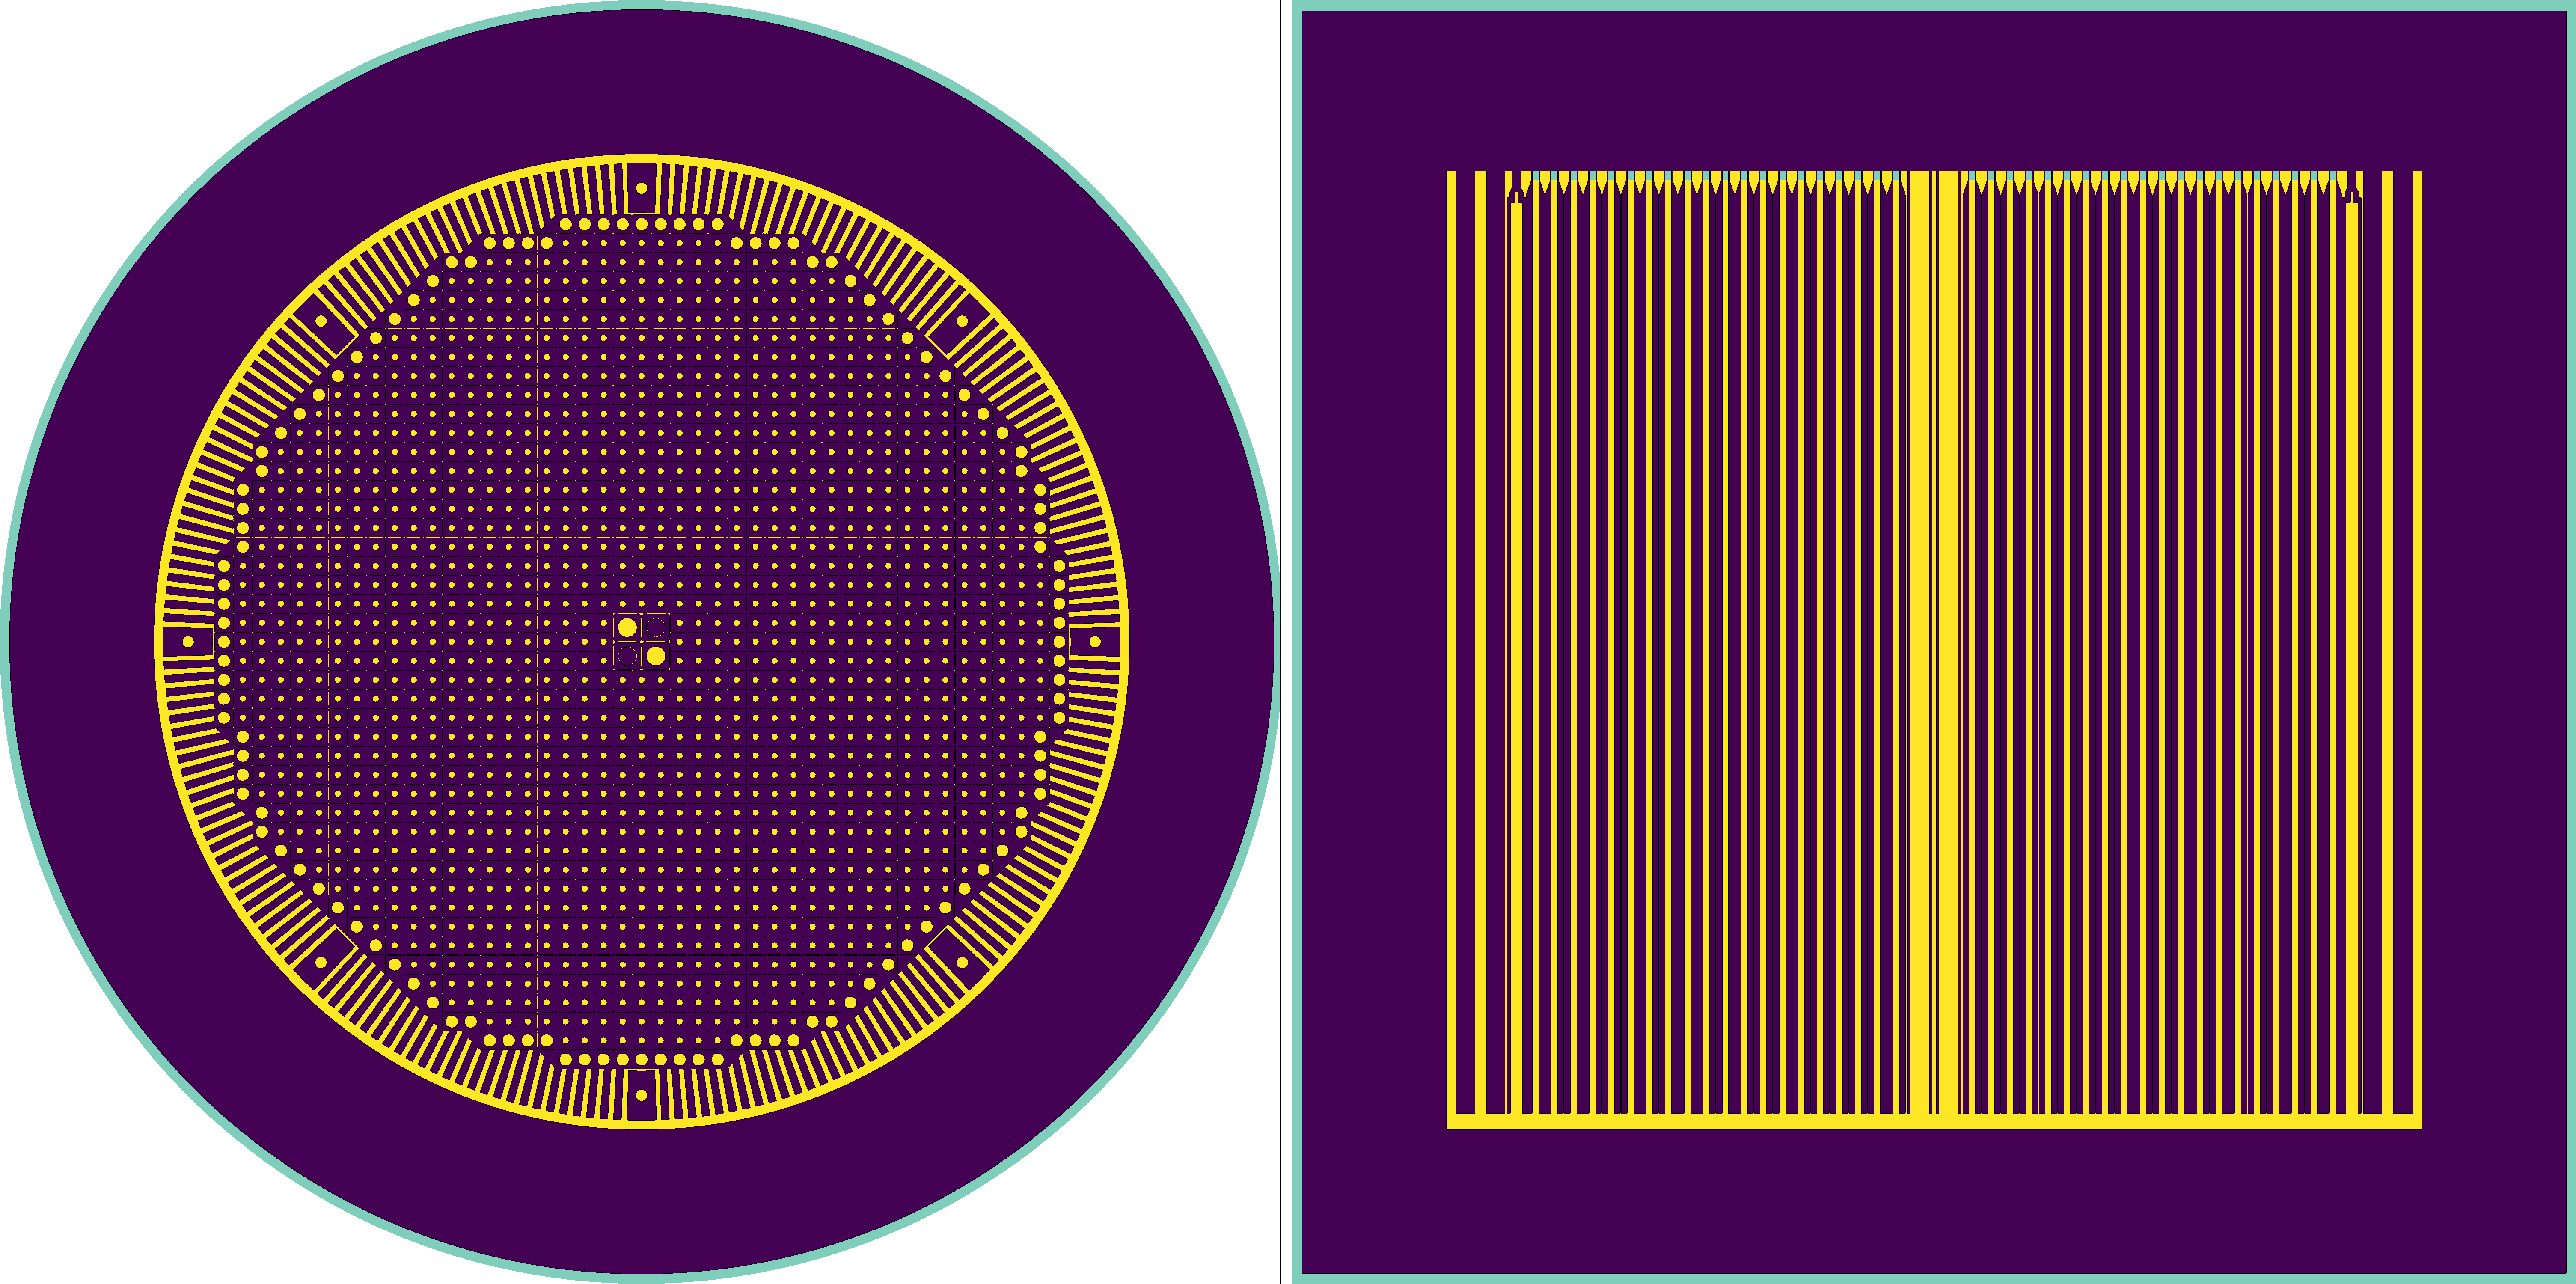
\includegraphics[width=\textwidth]{view_serpent.png}
  \caption{Plan and elevation views of SERPENT 2 \gls{MSBR} model developed in this work.}
  \label{fig:serpent_plan_view}
\end{figure}

Moreover, it was decided to remove and install the core graphite as an assembly rather than by individual blocks, because it is relatively easier for maintenance personnel and has lower probability of radioactive elements escape due to used blocks damage during removal. In addition, handling the core as an assembly also allows the replacement core to be carefully preassembled and tested under factory conditions.

There are eight symmetric graphite slabs with a width of 15.24 cm in zone II, one of which is illustrated in Figure~\ref{fig:serpent_zoneII}. The holes in the centers are for the core lifting rods used during the core replacement operations. These holes also allow a portion of the fuel salt to flow to the top of the vessel for cooling the top head and axial reflector. Figure~\ref{fig:serpent_zoneII} also demonstrates the 5.08-cm-wide annular space between the removable core graphite in zone II-B and the permanently mounted reflector graphite. This annulus consists entirely of fuel salt, provides space for moving the core assembly, helps compensate the elliptical dimensions of the reactor vessel, and serves to reduce the damaging flux at the surface of the graphite reflector blocks. In this work, all figures of the core were generated using the built-in SERPENT 2 plotter. All calculations presented in this study were performed using SERPENT 2 version 2.1.30 on Blue Waters’ XE6 nodes. 

\begin{figure}[t!] % replace 't' with 'b' to 
  \centering
  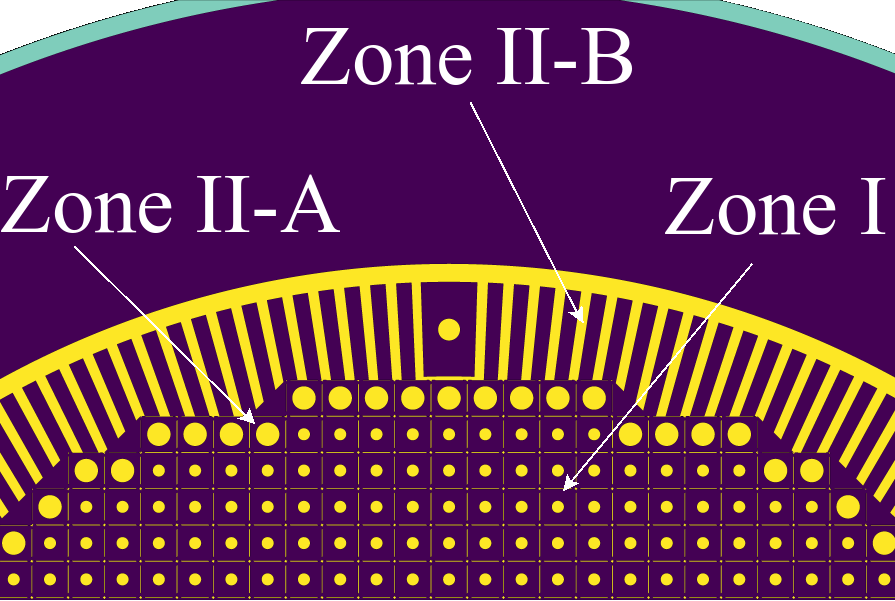
\includegraphics[width=\textwidth]{ser_zone_II.png}
  \caption{Detailed view of \gls{MSBR} zone II model.}
  \label{fig:serpent_zoneII}
\end{figure}

\subsubsection{Core zone I}
The central region of the core, called zone I, is made up of graphite elements, each $10.16$cm$\times$10.16cm$\times$396.24cm. Zone I has 4 channels for control rods: two for graphite rods which both regulate and shim during normal operation, and two for backup safety rods consisting of boron carbide clad to assure sufficient negative reactivity for emergency situations.

These graphite elements have a mostly rectangular shape with lengthwise ridges at each corner that leave space for salt flow elements. Various element sizes reduce the peak damage flux and power density in the center of the core to prevent local graphite damage. Zone I is well-moderated to achieve the desired fission power density. Figure~\ref{fig:I_element_ref} demonstrates the elevation and plan views of graphite elements of zone I \cite{robertson_conceptual_1971} and their SERPENT model \cite{rykhlevskii_full-core_2017}.
\begin{figure}[ht!] % replace 't' with 'b' to 
  \centering
  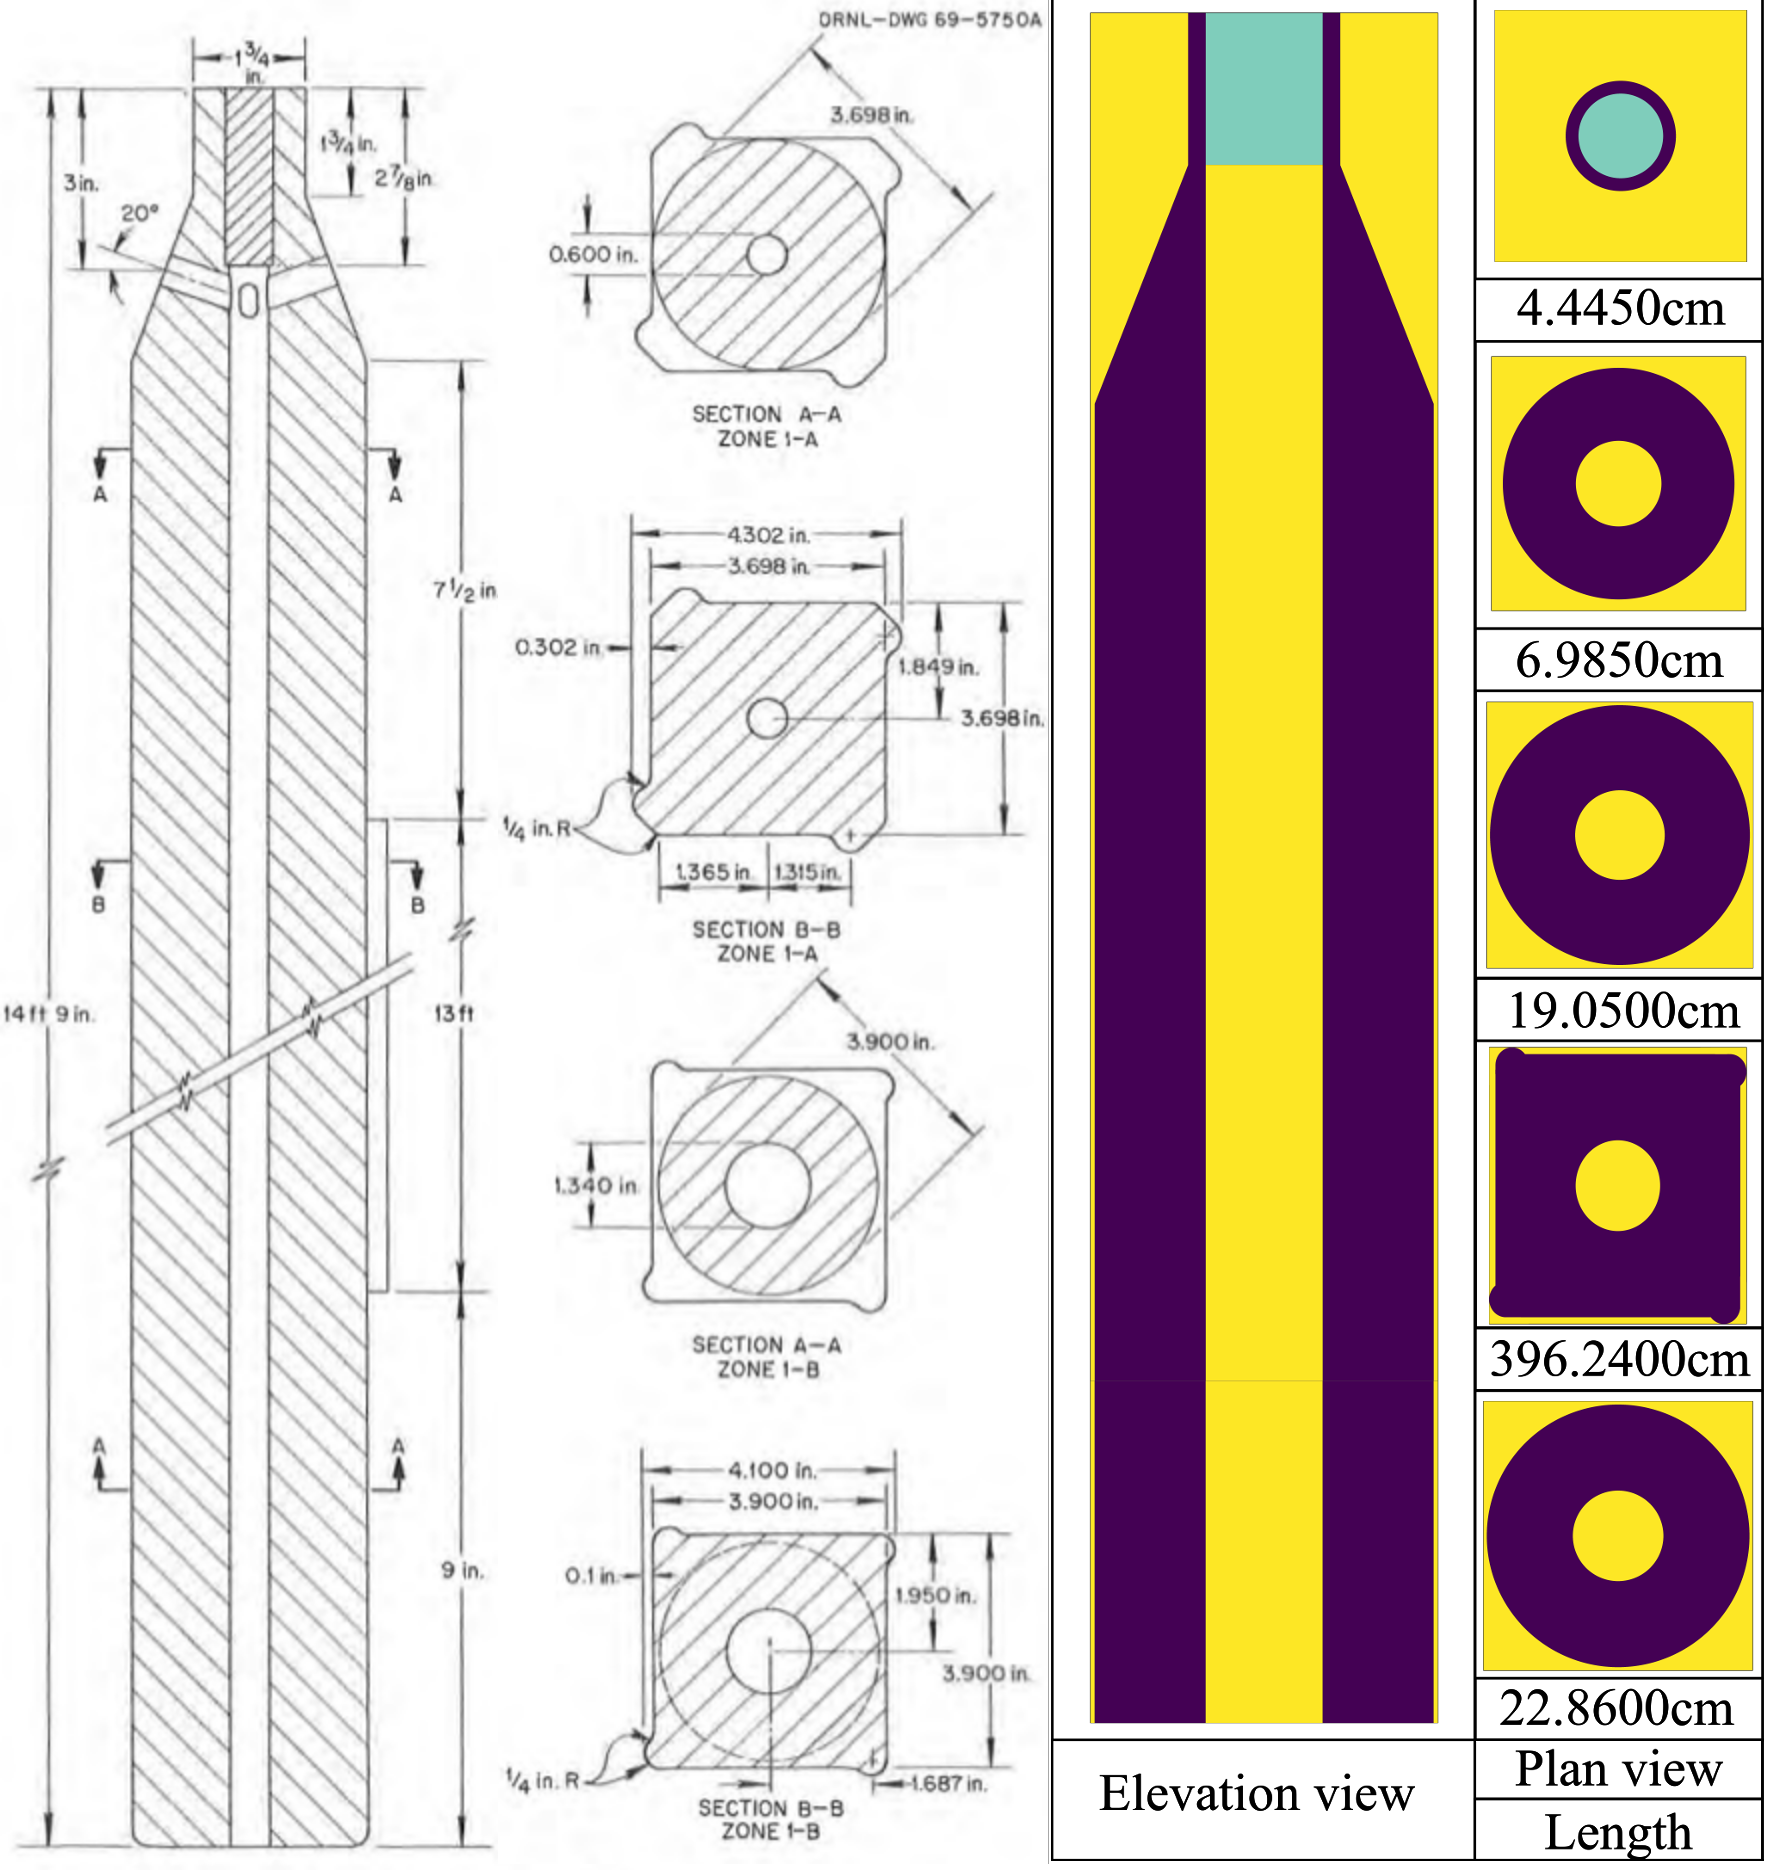
\includegraphics[width=\textwidth]{zone_I_element_ref.png}
  \caption{Graphite moderator elements for zone I \cite{robertson_conceptual_1971,rykhlevskii_full-core_2017}.}
  \label{fig:I_element_ref}
\end{figure}

\subsubsection{Core zone II}
Zone II which is undermoderated, surrounds zone I. Combined with the bounding radial reflector, zone II serves to diminish neutron leakage. This zone is formed of two kinds of elements: large-diameter fuel channels (zone II-A) and radial graphite slats (zone II-B). 

Zone II has 37\% fuel salt by volume and each element has a fuel channel diameter of 6.604cm. The graphite elements for zone II-A are prismatic and have elliptical-shaped dowels running axially between the prisms and needed to isolate the fuel salt flow in zone I from that in zone II. Figure~\ref{fig:II_element_ref} shows shape and dimensions of these graphite elements and their SERPENT model. Zone II-B elements are rectangular slats spaced far enough apart to provide the 0.37 fuel salt volume fraction. The reactor zone II-B graphite 5.08cm-thick slats vary in the radial dimension (average width is 26.67cm) as shown in figure~\ref{fig:serpent_zoneII}. Zone II serves as a blanket to achieve the best performance: a high breeding ratio and a low fissile inventory. The neutron energy spectrum in zone II is made harder to enhance the rate of thorium resonance capture relative to the fission rate, thus limiting the neutron flux in the outer core zone and reducing the neutron leakage \cite{robertson_conceptual_1971}. 

The main challenge was to accurately represent zone II-B because it has irregular elements with sophisticated shapes. From the \gls{ORNL} report \cite{robertson_conceptual_1971}, the suggested design of zone II-B has 8 irregularly-shaped graphite elements every 45$^\circ$ as well as salt channels. These graphite elements were simplified into right-circular cylindrical shapes  with central channels. Figure~\ref{fig:serpent_zoneII} illustrates this core region in the SERPENT model. The volume of fuel salt in zone II was kept exactly 37\%, so that this simplification did not considerably change the core neutronics. This is the only simplification made to the \gls{MSBR} geometry in this work. 

\begin{figure}[ht!] % replace 't' with 'b' to 
  \centering
  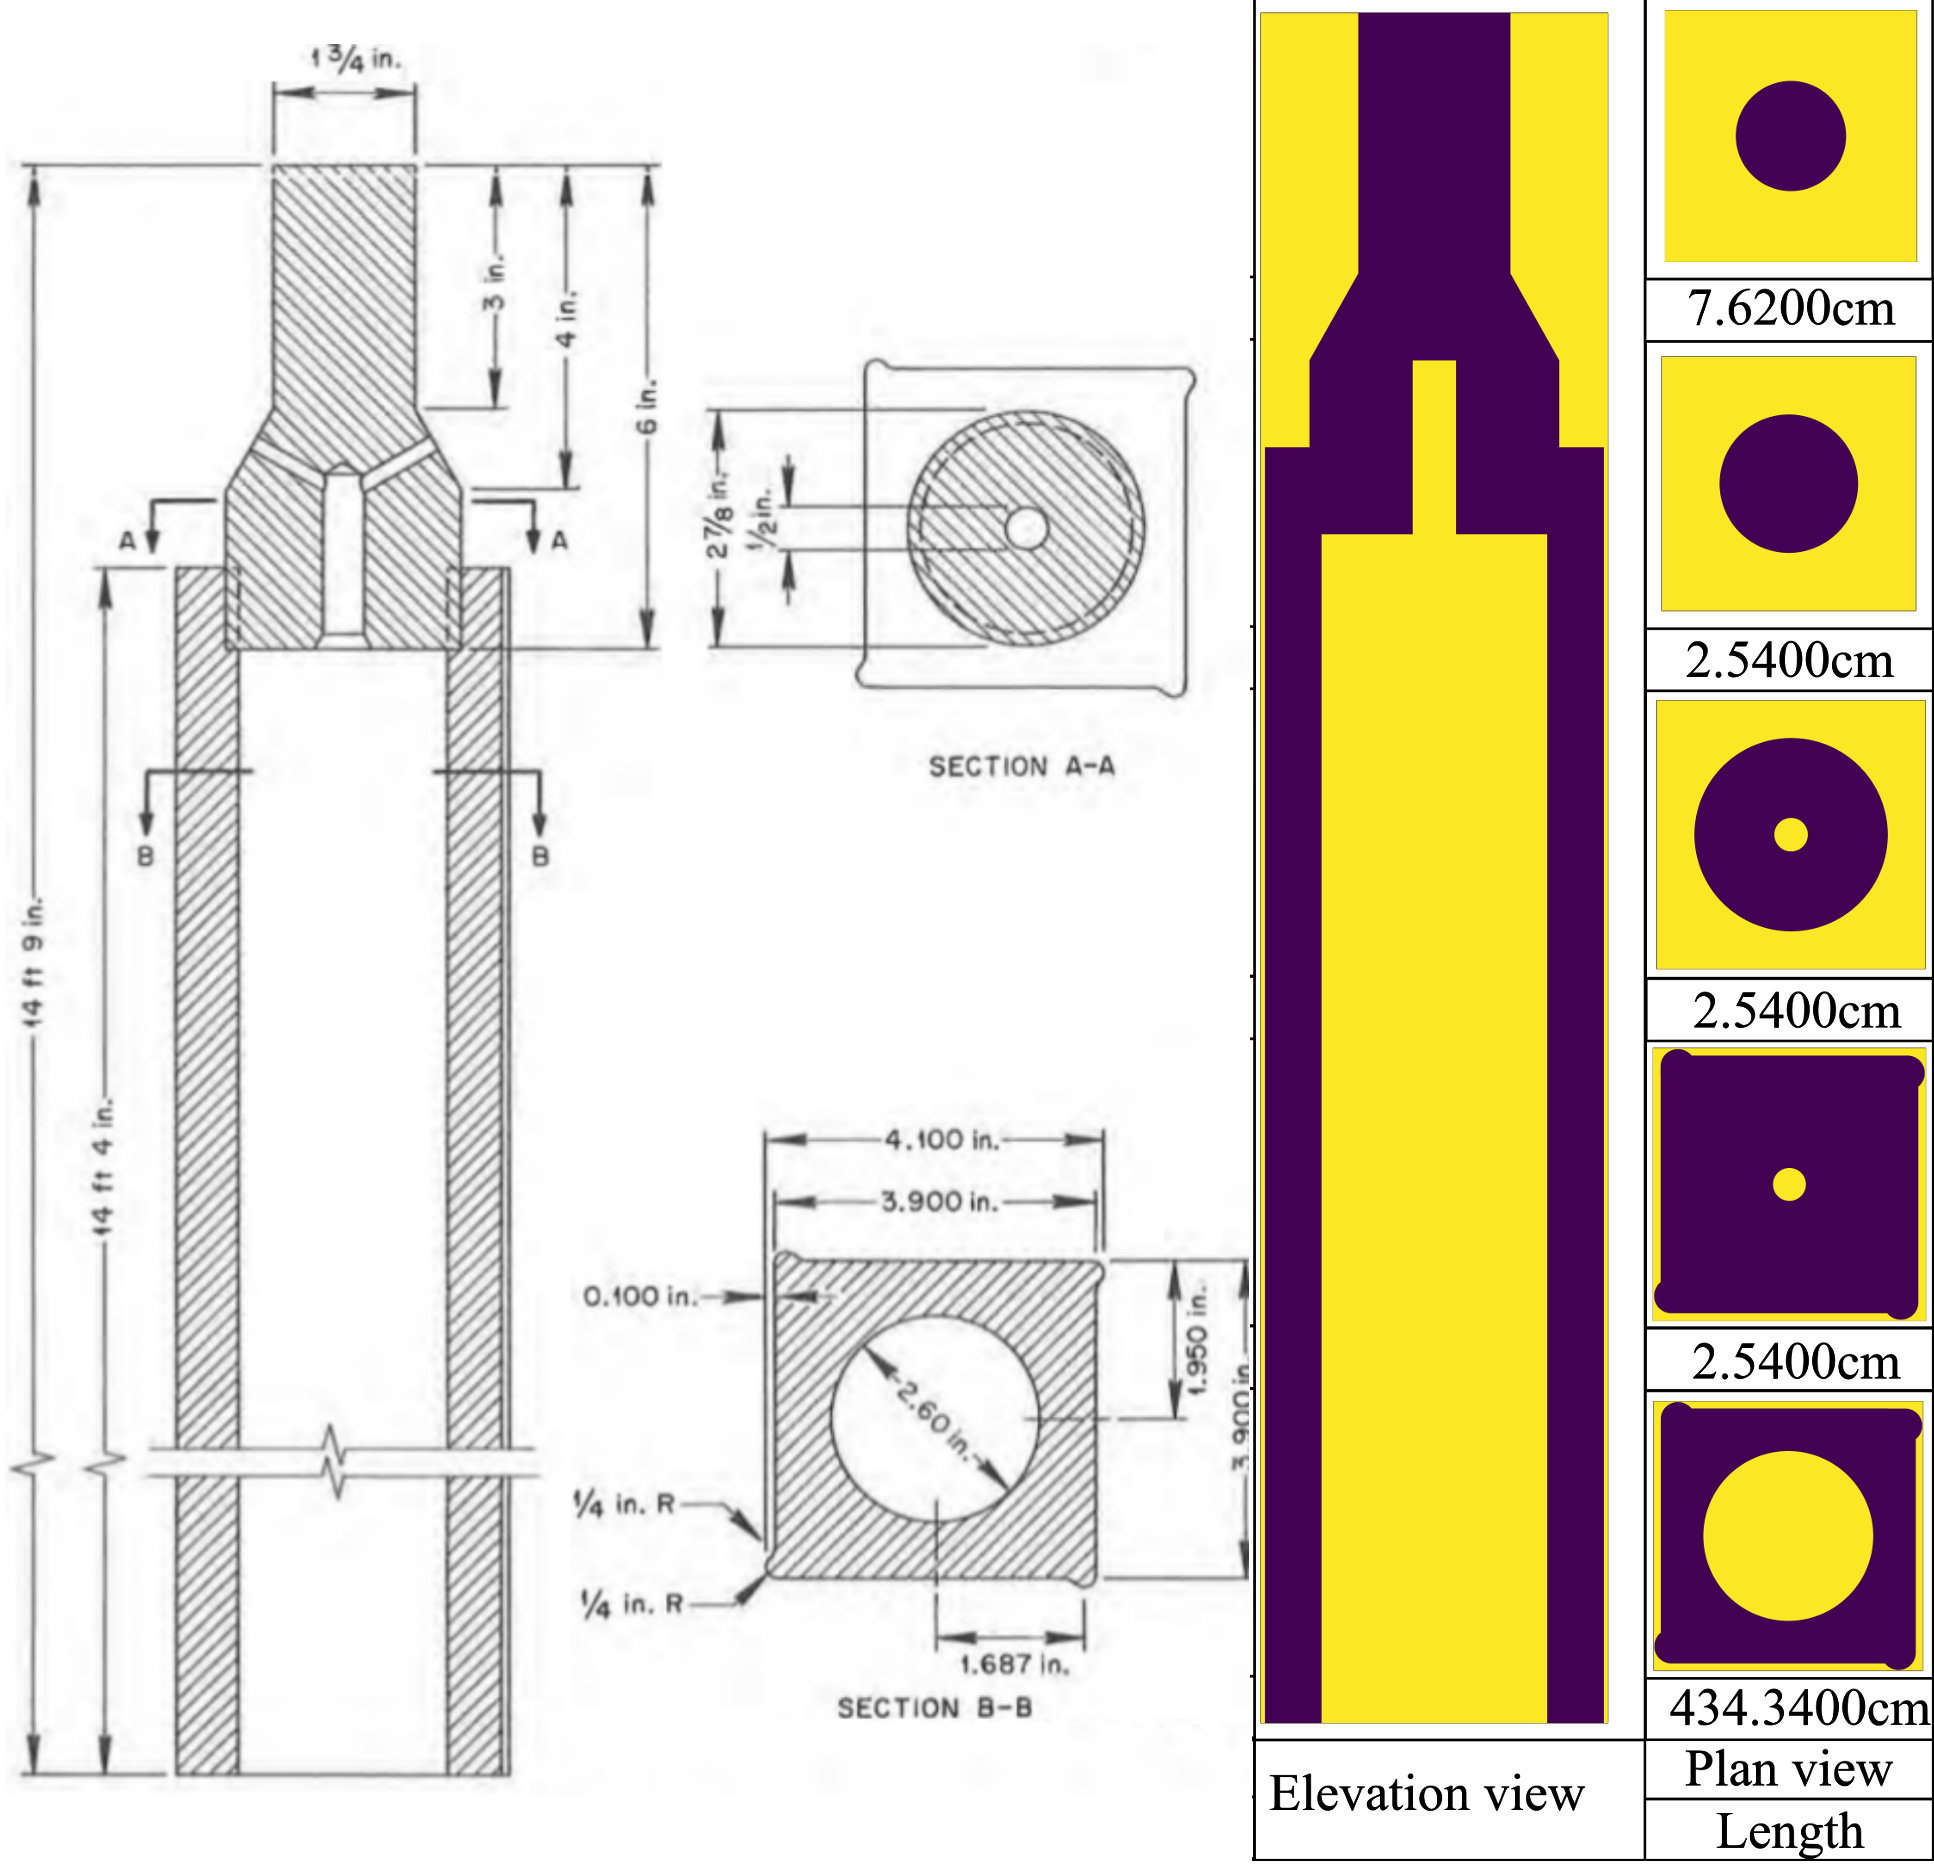
\includegraphics[width=\textwidth]{zone_II_element_ref.png}
  \caption{Graphite moderator elements for zone II-A \cite{robertson_conceptual_1971,rykhlevskii_full-core_2017}.}
  \label{fig:II_element_ref}
\end{figure}

\subsubsection{Material composition and normalization parameters}
The fuel salt, the reactor graphite, and the modified Hastelloy-N\footnote{ Hastelloy-N is very common in reactors now but have been studied and developed at \gls{ORNL} in a program that started in 1950s.} are materials unique of the \gls{MSBR} and were created at \gls{ORNL}. The initial fuel salt used the same density (3.35 g/cm$^3$) and composition LiF-BeF$_2$-ThF$_4$-$^{233}$UF$_4$ (71.75-16-12-0.25 mole \%) as the \gls{MSBR} design \cite{robertson_conceptual_1971}. The lithium in the molten salt fuel is fully enriched in $^{7}$Li because $^{6}$Li is a very strong neutron poison and becomes tritium upon neutron capture. 

For cross section generation, JEFF-3.1.2 neutron library was employed \cite{oecd/nea_data_bank_jeff-3.1.2_2014}. The specific temperature was fixed for each material to correctly model the Doppler-broadening of resonance peaks when SERPENT generates the problem-dependent nuclear data library. The isotopic composition of each material at the initial state was described in detail in the MSBR conceptual design study \cite{robertson_conceptual_1971} and has been applied to SERPENT model without any modification. Table~\ref{tab:msbr_tab} is a summary of the major \gls{MSBR} parameters used by this model \cite{robertson_conceptual_1971}. 

%%%%%%%%%%%%%%%%%%%%%%%%%%%%%%%%%%%%%%%%
\begin{table}[h!]
        %\centering
        \caption{Summary of principal data for MSBR \cite{robertson_conceptual_1971}.}
        \begin{tabularx}{\textwidth}{ s  s}
        \hline
                Thermal capacity of reactor           		& 2250 MW(t)
                \\ 
                Net electrical output                 		& 1000 MW(e) 
                \\  
                Net thermal efficiency        				& 44.4\%
                \\  
                Salt volume fraction in central zone I		& 0.13
                \\ 
                Salt volume fraction in outer zone II       & 0.37
                \\ 
                Fuel salt inventory (Zone I)                & 8.2 m$^3$	
                \\ 
                Fuel salt inventory (Zone II)               & 10.8 m$^3$	
                \\ 
                Fuel salt inventory (annulus)               & 3.8 m$^3$	
                \\  
                Total fuel salt inventory                   & 48.7 m$^3$	
                \\ 
                Fissile mass in fuel salt                   & 1303.7 kg	
                \\ 
                Fuel salt components                  & 
                LiF-BeF$_2$-ThF$_4$-$^{233}$UF$_4$	
                \\  
                Fuel salt composition                 & 
                71.75-16-12-0.25 mole\%
                \\
                Fuel salt density                    & 
                3.35 g/cm$^3$
                \\ \hline
        \end{tabularx}
        \label{tab:msbr_tab}
\end{table}
%%%%%%%%%%%%%%%%%%%%%%%%%%%%%%%%%%%%%%%%%%%%%%%%

\subsection{Online reprocessing method}
Removing specific chemical elements from a molten salt is a complicated task that requires intelligent design (e.g., chemical separations equipment design, fuel salt flows to equipment) and has a considerable economic cost. All liquid-fueled \gls{MSR} designs involve varying levels of online fuel processing. Minimally, volatile gaseous fission products (e.g. Kr, Xe) escape from the fuel salt during routine reactor operation and must be captured. Additional systems might be used to enhance removal of those elements. Most designs also call for the removal of noble and rare earth metals from the core since these metals act as neutron poisons. Some designs suggest a more complex list of elements to process (figure ~\ref{fig:periodic_tab}), including the temporary removal of protactinium from the salt or other regulation of the actinide inventory in the fuel salt \cite{ahmad_neutronics_2015}.

\begin{figure}[htp!] % replace 't' with 'b' to 
  \centering
  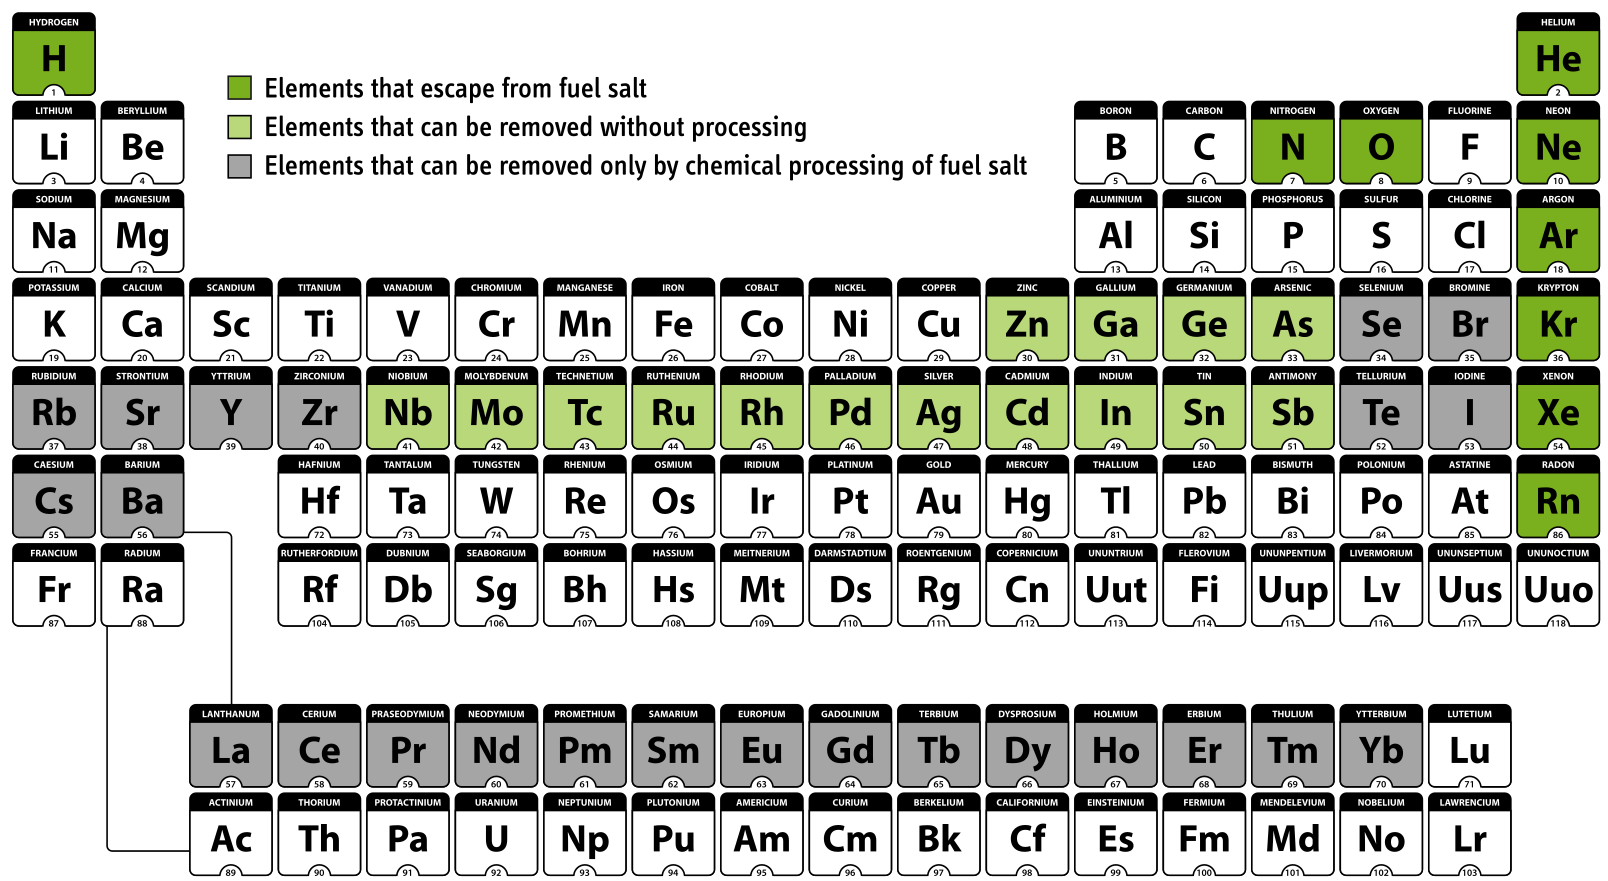
\includegraphics[width=\textwidth]{periodic_map.png}
  \caption{Processing options for \gls{MSR} fuels \cite{ahmad_neutronics_2015}.}
  \label{fig:periodic_tab}
\end{figure}

\subsubsection{Fuel material flows}
The $^{232}$Th in the fuel absorbs thermal neutrons and produces $^{233}$Pa which then decays into the fissile $^{233}$U. Furthermore, the \gls{MSBR} design requires online reprocessing to remove all poisons (e.g. $^{135}$Xe), noble metals, and gases (e.g. $^{75}$Se, $^{85}$Kr) every 20 seconds. Protactinium presents a challenge, since it has a large absorption cross section in the thermal energy spectrum. Accordingly, $^{233}$Pa is continuously removed from the fuel salt into a protactinium decay tank to allow $^{233}$Pa to decay to $^{233}$U without poisoning the reactor. The reactor reprocessing system is designed to separate $^{233}$Pa from the molten-salt fuel over 3 days, hold it while $^{233}$Pa decays into $^{233}$U, and return it back to the primary loop. This feature allows the reactor to avoid neutron losses to protactinium, keeps fission products to a very low level, and increases the efficiency of $^{233}$U breeding. Table~\ref{tab:reprocessing_list} summarizes full list of nuclides and the cycle times used for modeling salt treatment and separations \cite{robertson_conceptual_1971}. 

%%%%%%%%%%%%%%%%%%%%%%%%%%%%%%%%%%%%%%%%
\begin{table}[ht!]
        \centering
        \caption{The effective cycle times for protactinium and fission products removal (reproduced from \cite{robertson_conceptual_1971}).}
        \begin{tabularx}{\textwidth}{ x | s | x }
        \hline 
        Processing group & \qquad\qquad\qquad Nuclides & Cycle time (at full power) \\ \hline 
        Rare earths & Y, La, Ce, Pr, Nd, Pm, Sm, Gd & 50 days \\ 
        \qquad & Eu & 500 days \\ 
        Noble metals & Se, Nb, Mo, Tc, Ru, Rh, Pd, Ag, Sb, Te & 20 sec \\
        Seminoble metals & Zr, Cd, In, Sn & 200 days \\
        Gases & Kr, Xe & 20 sec \\ 
        Volatile fluorides & Br, I & 60 days \\
        Discard & Rb, Sr, Cs, Ba & 3435 days \\ 
        Salt discard & Th, Li, Be, F & 3435 days \\ 
        Protactinium & $^{233}$Pa & 3 days \\ 
        Higher nuclides & $^{237}$Np, $^{242}$Pu & 16 years \\  \hline
        \end{tabularx}
        %\footnotetext{Chemical processing plant and gas separation system removing chemical elements (not isotopes) only. Isotopes instead of elements listed because other isotopes are short-lived and might be ignored.}
        \label{tab:reprocessing_list}
\end{table}
Th removal rates vary among nuclides in this reactor concept which dictate the necessary resolution of depletion calculations. If the depletion time intervals are very short, an enormous number of depletion steps are required to obtain the equilibrium composition. On the other hand, if the depletion  calculation time interval is too long, the impact of short-lived fission products is not captured. To compromise, the time interval for depletion calculations in this model was selected as 3 days to correlate with the removal interval of $^{233}$Pa and $^{232}$Th was continuously added to maintain the initial mass fraction of $^{232}$Th.

\subsubsection{The SaltProc modeling and simulation code}
The SaltProc tool \cite{andrei_rykhlevskii_arfc/saltproc:_2018} is designed to expand SERPENT 2
 depletion capabilities for modeling liquid-fueled \gls{MSR} for continuous reprocessing.
The Python package uses HDF5 \cite{the_hdf_group_hierarchical_1997} to store data, and the Nuclear Engineering Toolkit PyNE \cite{scopatz_pyne:_2012}
for SEPRENT output file parsing and nuclide naming. It is an open-source tool that uses a semi-continuous approach to 
simulate continuous feeds and removals in the \gls{MSR}. 

The tool structure and capabilities of SaltProc are similar to ChemTriton tool for SCALE
developed in \gls{ORNL} \cite{powers_new_2013}. SaltProc is coupled with Monte Carlo SERPENT 2
software which allows to simulate online reprocessing for irregular full-core geometry with 
high level of fidelity.  The primary function of SaltProc is to manage material streams while
SERPENT 2 performs most of the computationally heavy work, namely neutron transport and depletion
calculations. Saltproc is defined as a 
python class, where each material stream is defined as a isotopic atomic density
vector variable. This allows tracking of time-sensitive material streams such as the
$^{233}$Pa tank in the \gls{MSBR}. The user can define the reprocessing parameters, such as the 
reprocessing interval and removal efficiency.  In addition, SaltProc provides a set of functions 
for each stream: read and write isotopic data in/from database, separate out specific isotopes 
from stream with defined efficiency, feed in specific isotopes to stream, and maintain constant 
number density of specific nuclide in the core. These attributes and functions are crucial to 
simulate the operation of a complex, multi-zone, multi-fluid \gls{MSR} and are universal for 
myriad reactor systems.

Saltproc is currently in active development in Github (https://github.com/ arfc/saltproc), and has unit tests and Travis continuous integration for sustainable development. There is also documentation
generated through Sphinx document generator for ease of use. We plan to implement
user-defined reprocessing scheme definition, two-region \gls{MSR} modeling capabilities,
and decay modeling in future releases.

Figure~\ref{fig:saltproc_flow} illustrates the  online reprocessing simulation algorithm the 
coupled SaltProc and SERPENT 2. To perform a depletion step,
SaltProc reads an external SERPENT 2 template file which is defined by the user. This file 
contains input cards with parameters such as geometry,
moderator and construction materials isotopic composition, neutron population, criticality 
cycles, total heating power, and boundary conditions.
After the depletion calculation, SaltProc reads the depleted fuel composition file (\texttt{
.bumat1}) and stores the depleted
composition isotopic vector in an HDF5 database. SaltProc only stores and edits the isotopic 
composition of the fuel stream,
which makes SaltProc a flexible tool to model any geometry: an infinite medium, a unit cell, a 
multi-zone simplified assembly, or a full core.
This flexibiliity allows the user to perform simulations of varying fidelity and computational 
intensity.
\begin{figure}[ht!] % replace 't' with 'b' to 
  \centering
  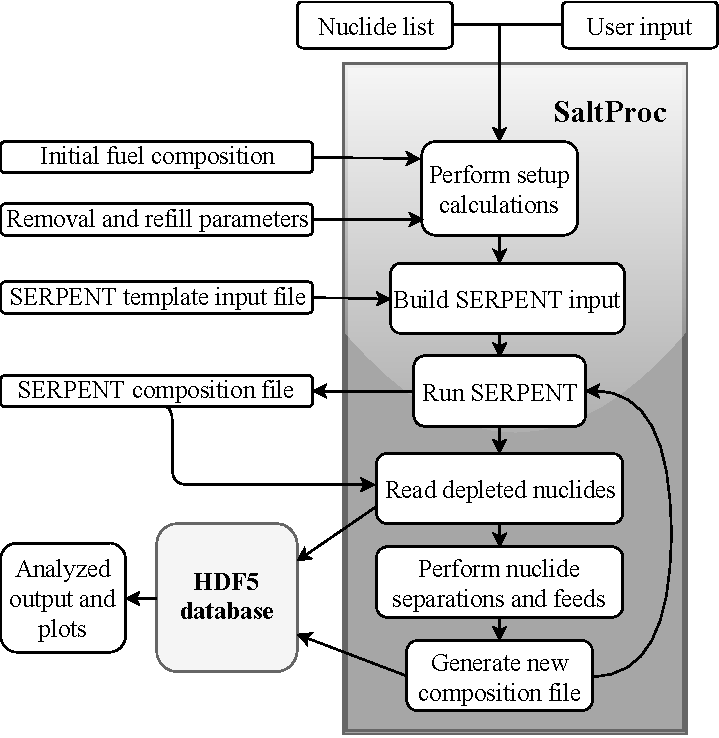
\includegraphics[width=0.75\textwidth]{saltproc_flowchart.pdf}
  \caption{Flow chart for the Saltproc python-based tools.}
  \label{fig:saltproc_flow}
\end{figure}
SaltProc can manage as many material streams as desired. It also may work with multiple depletion 
materials. At the end of a each depletion step, SaltProc reads the depleted compositions and tracks each material stream individually. Following this, it applies chemical separation functions to fuel stream vectors. These vectors then form a matrix (isotopics x timesteps) which SaltProc stores in an HDF5 database and prints into the SERPENT 2 composition file for the next depletion calculation.

Saltproc datasets are timseries, meaning that every value is recorded every timestep. The 
datasets SaltProc produces are listed below,
where the values inside the parenthesis are the dataset sizes:

\begin{itemize}
    \item \texttt{core adensity before reproc} (number of isotopes x timesteps)
    \item \texttt{core adensity after reproc} (number of isotopes x timesteps)
    \item \texttt{Keff\_BOC} (1 x timesteps)
    \item \texttt{Keff\_EOC} (1 x timesteps)
    \item \texttt{Th tank adensity} (number of isotopes x timesteps)
    \item \texttt{iso codes} (number of isotopes x 1)
\end{itemize}

Liquid-fueled \gls{MSBR} design in this work focuses on the state of the core at an equilibrium condition, after fission products have built up in the fuel salt during years if operation. Isotopic composition of the fuel salt continues change slightly even after decades of operation, but the dominant nuclides that have significant impact to the neutronic behavior tend to reach an equilibrium concentration (e.g., vary less than 1\% over several years). In contrast, from the startup of an \gls{MSBR} until the equilibrium condition, the fuel salt composition undergoes significant changes (e.g., changes in fission products, minor actinides, and fissile materials number density). During this period, the material feeds and removals should be optimized for the fastest \gls{MSBR} transition to an equilibrium state. A faster transition simplifies the reactor operation because, at equilibrium, the fissile and fertile feed rates, fission product removal rates, and corresponding core safety parameters are constant in time.

In addition, SaltProc is able to define time-dependent material feed and removal rates to investigate the their impacts. These rates need not be constant in SaltProc. They can be defined as piecewise functions or set to respond conditions in the core. For instance, SaltProc might increase the fissile material feeding rate if the effective multiplication factor, $k_{eff}$, falls below a specific limit (e.g., 1.002).
These capabilities allow SaltProc to analyze fuel cycle of a generic liquid-fueled \gls{MSR}. In summary, the development approach of SaltProc focused on producing a generic, flexible and expandable tool to give the SERPENT 2 Monte Carlo code the ability to conduct advanced in-reactor fuel cycle analysis as well as simulate a myriad of online refueling and fuel reprocessing systems.

\FloatBarrier
\section{Results}
The SaltProc online reprocessing simulation package is demonstrated in four 
applications: (1) analyzing  \gls{MSBR} neutronics and fuel cycle to find the 
equilibrium core composition and core depletion, (2) studying operational and 
safety parameters evolution during \gls{MSBR} operation, (3) demonstrating that 
in a single-fluid two-region \gls{MSBR} conceptual design the undermoderated 
outer core zone II works as a virtual ``blanket", reduces neutron leakage and 
improves breeding ratio due to neutron energy spectral shift, and (4) 
determining the effect of fission product removal on the core neutronics.

The neutron population per cycle and the number of active/inactive cycles were 
chosen to obtain balance between reasonable uncertainty for a transport problem 
($\leq$ 15 pcm\footnote{ 1 pcm = 10$^{-5}\Delta k_{eff}/k_{eff}$} for effective 
multiplication factor) and computational time. The \gls{MSBR} depletion and 
safety parameter computations were performed on 64 Blue Waters XK7 nodes (two 
AMD 6276 Interlagos CPU per node, 16 floating-point Bulldozer core units per 
node or 32 ``integer" cores per node, nominal clock speed is 2.45 GHz). The 
total computational time for calculating the equilibrium composition was 
approximately 9,900 node-hours (18 core-years.)

\subsection{Effective multiplication factor}
Figure~\ref{fig:keff} shows the effective multiplication factors 
obtained using SaltProc and SERPENT 2. The effective multiplication factors were 
calculated after removing fission products listed in 
Table~\ref{tab:reprocessing_list} and adding the fertile material at the end of 
cycle time (3 days for this work). The effective multiplication 
factor fluctuates significantly as a result of the batch-wise nature of this 
online reprocessing strategy. 

\begin{figure}[ht!] 
  \centering
  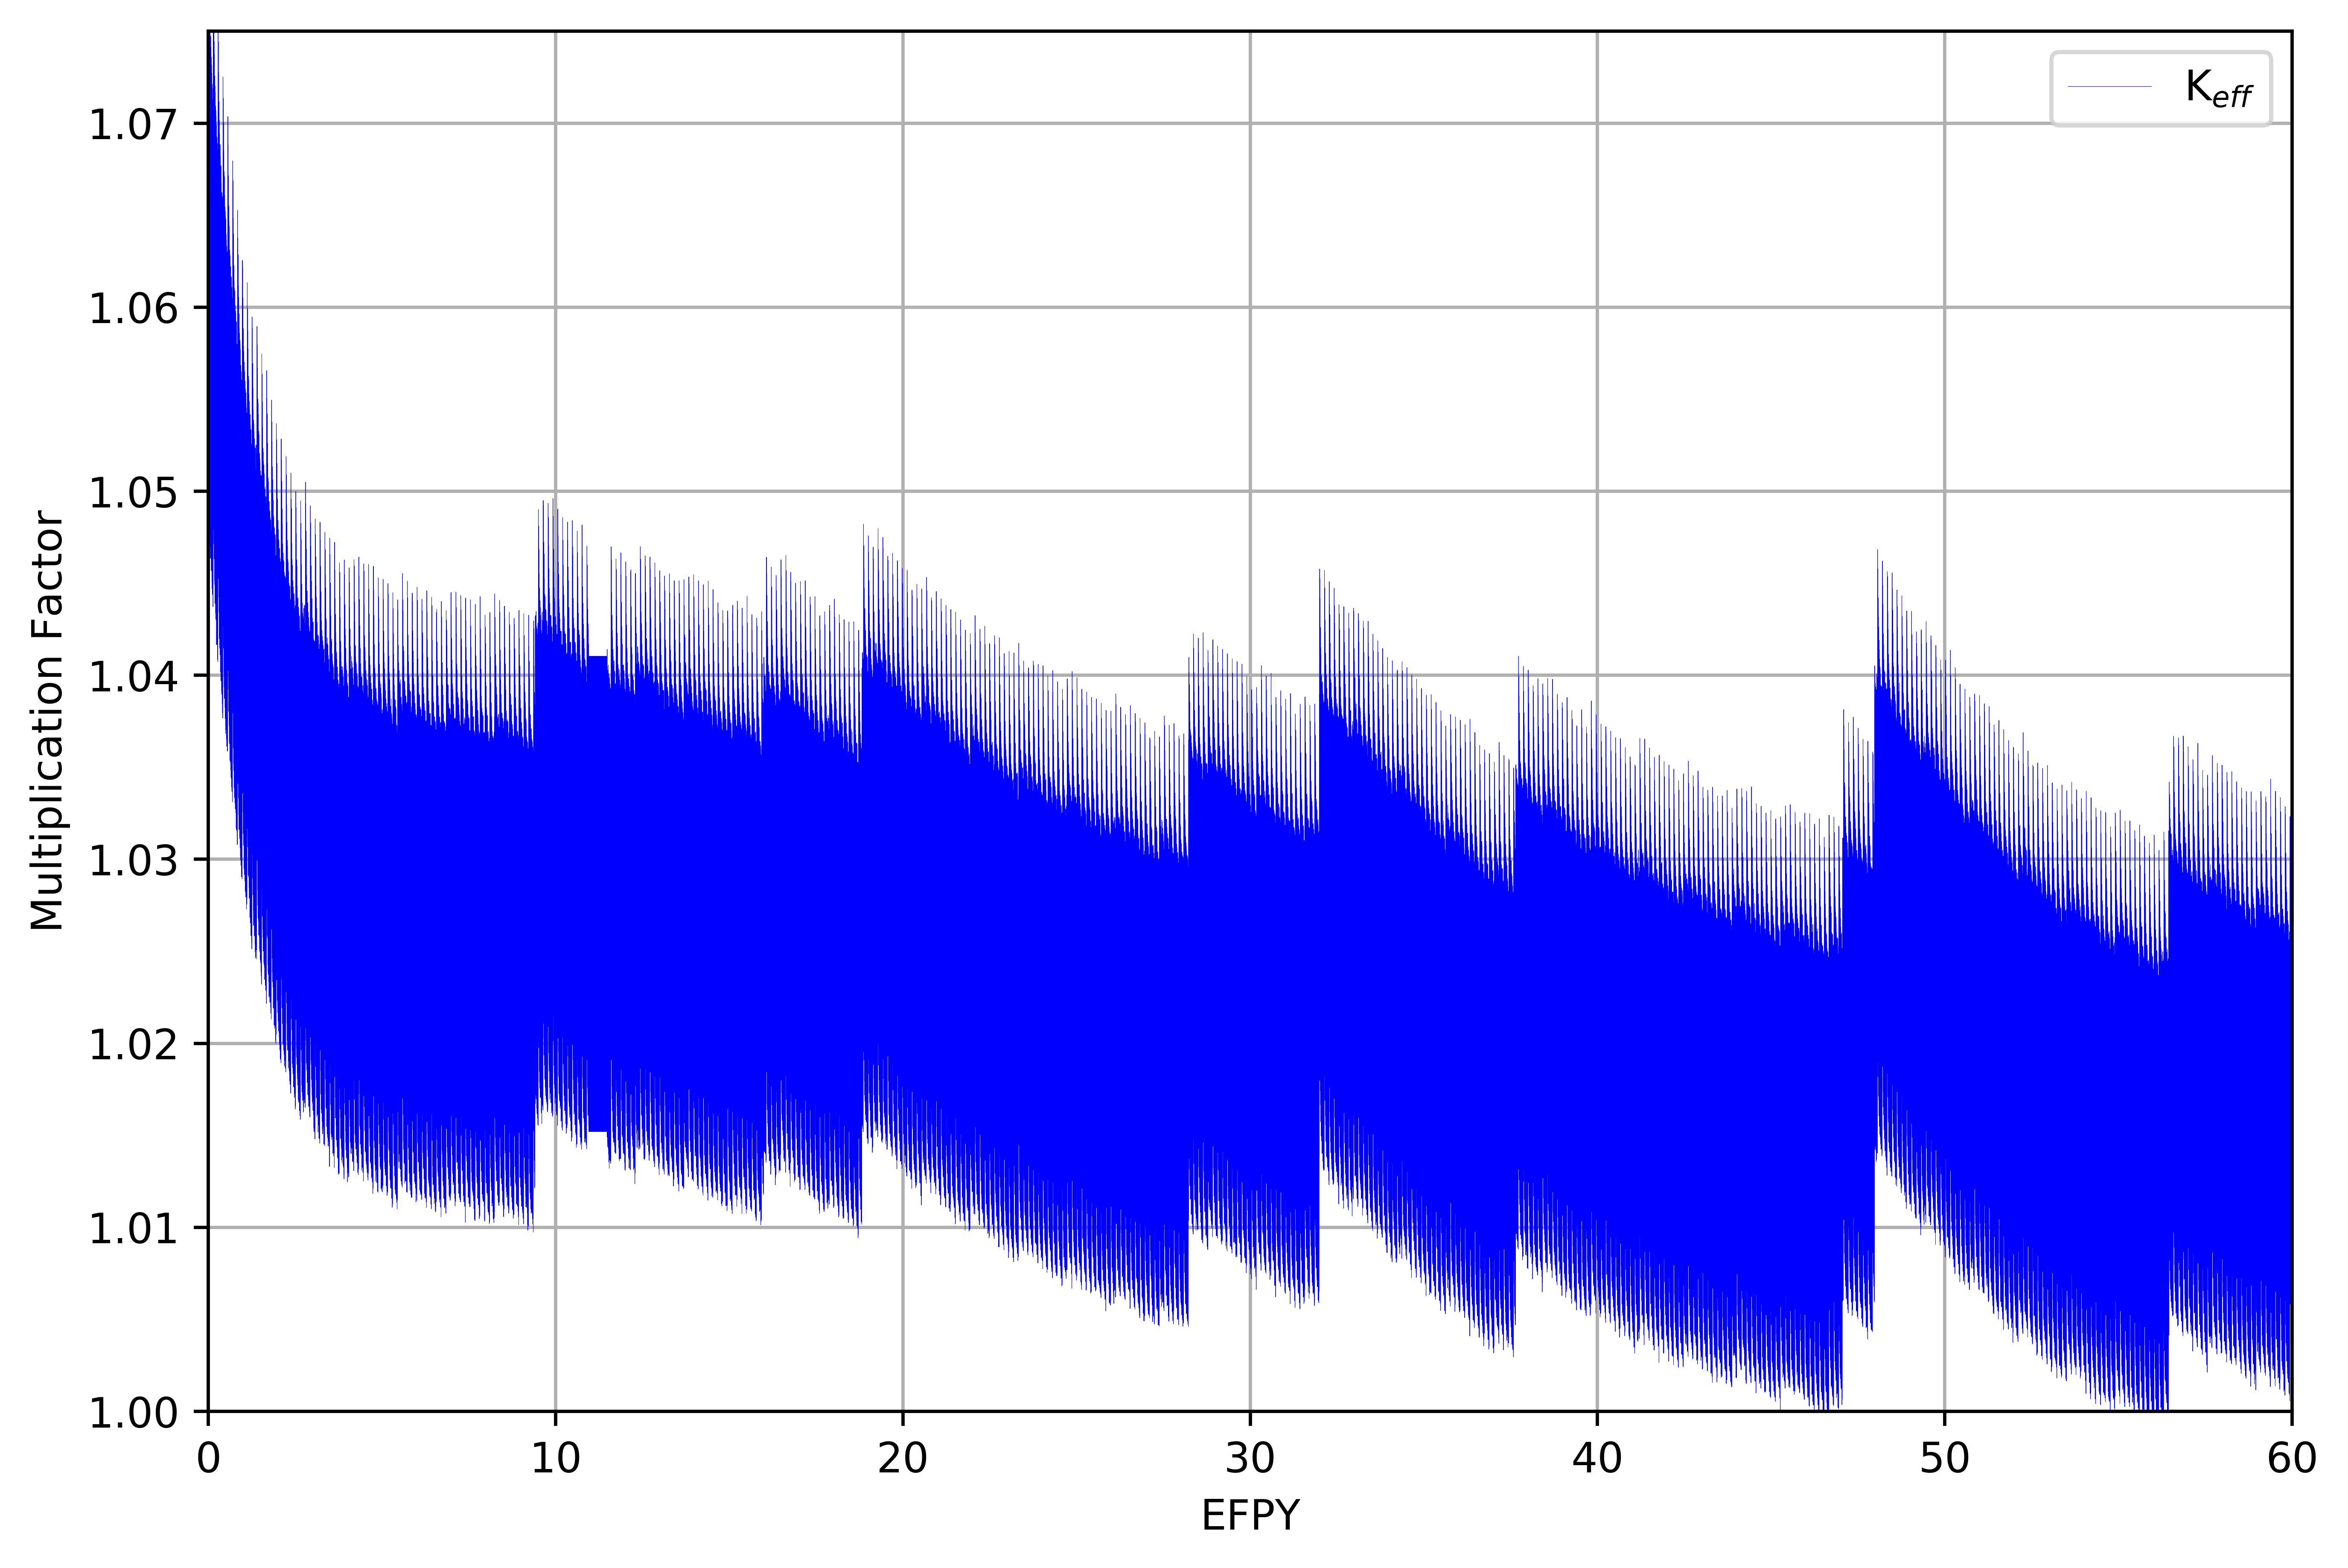
\includegraphics[width=\textwidth]{keff.png}
  \caption{Effective multiplication factor dynamics for full-core \gls{MSBR} 
  model over a 60-year reactor operation lifetime.}
  \label{fig:keff}
\end{figure}

First, SERPENT calculates the effective multiplication factor for the beginning 
of the cycle (there is fresh fuel composition at the first step). Next, it 
computes the new fuel salt composition at the end of a 3-day depletion. The 
corresponding effective multiplication factor is much smaller than the previous 
one. Finally, SERPENT calculates $k_{eff}$ for the depleted composition after 
applying feeds and removals. The $K_{eff}$ increases accordingly since major reactor 
poisons (e.g. Xe, Kr) are removed, while fresh fissile material ($^{233}$U) 
from the protactinium decay tank is added.  

Additionally, the presence of rubidium, strontium, cesium, and barium in the 
core are disadvantageous to reactor physics. In fact, the removal of these elements 
every 3435 days causes the multiplication factor to jump by approximately 450 
pcm, and limits using the batch approach for online reprocessing simulations. 
Overall, the effective multiplication factor gradually decreases from 1.075 to 
$\approx$1.02 at equilibrium after approximately 6 years of irradiation. 

\subsection{Fuel salt composition dynamics}
The analysis of the fuel salt composition evolution provides more comprehensive 
information about the equilibrium state. Figure~\ref{fig:adens_eq} shows the number 
densities of major nuclides which have a strong influence on the reactor core 
physics. The concentration of $^{233}$U, $^{232}$Th, $^{233}$Pa, and $^{232}$Pa in 
the fuel salt change insignificantly after approximately 2500 days of operation. 
In particular, the $^{233}$U number density fluctuates by less than 0.8\% between
 16 and 20 years of operation. Hence, a quasi-equilibrium state was 
achieved after 16 years of reactor operation.
\begin{figure}[ht!] % replace 't' with 'b' to 
  \centering
  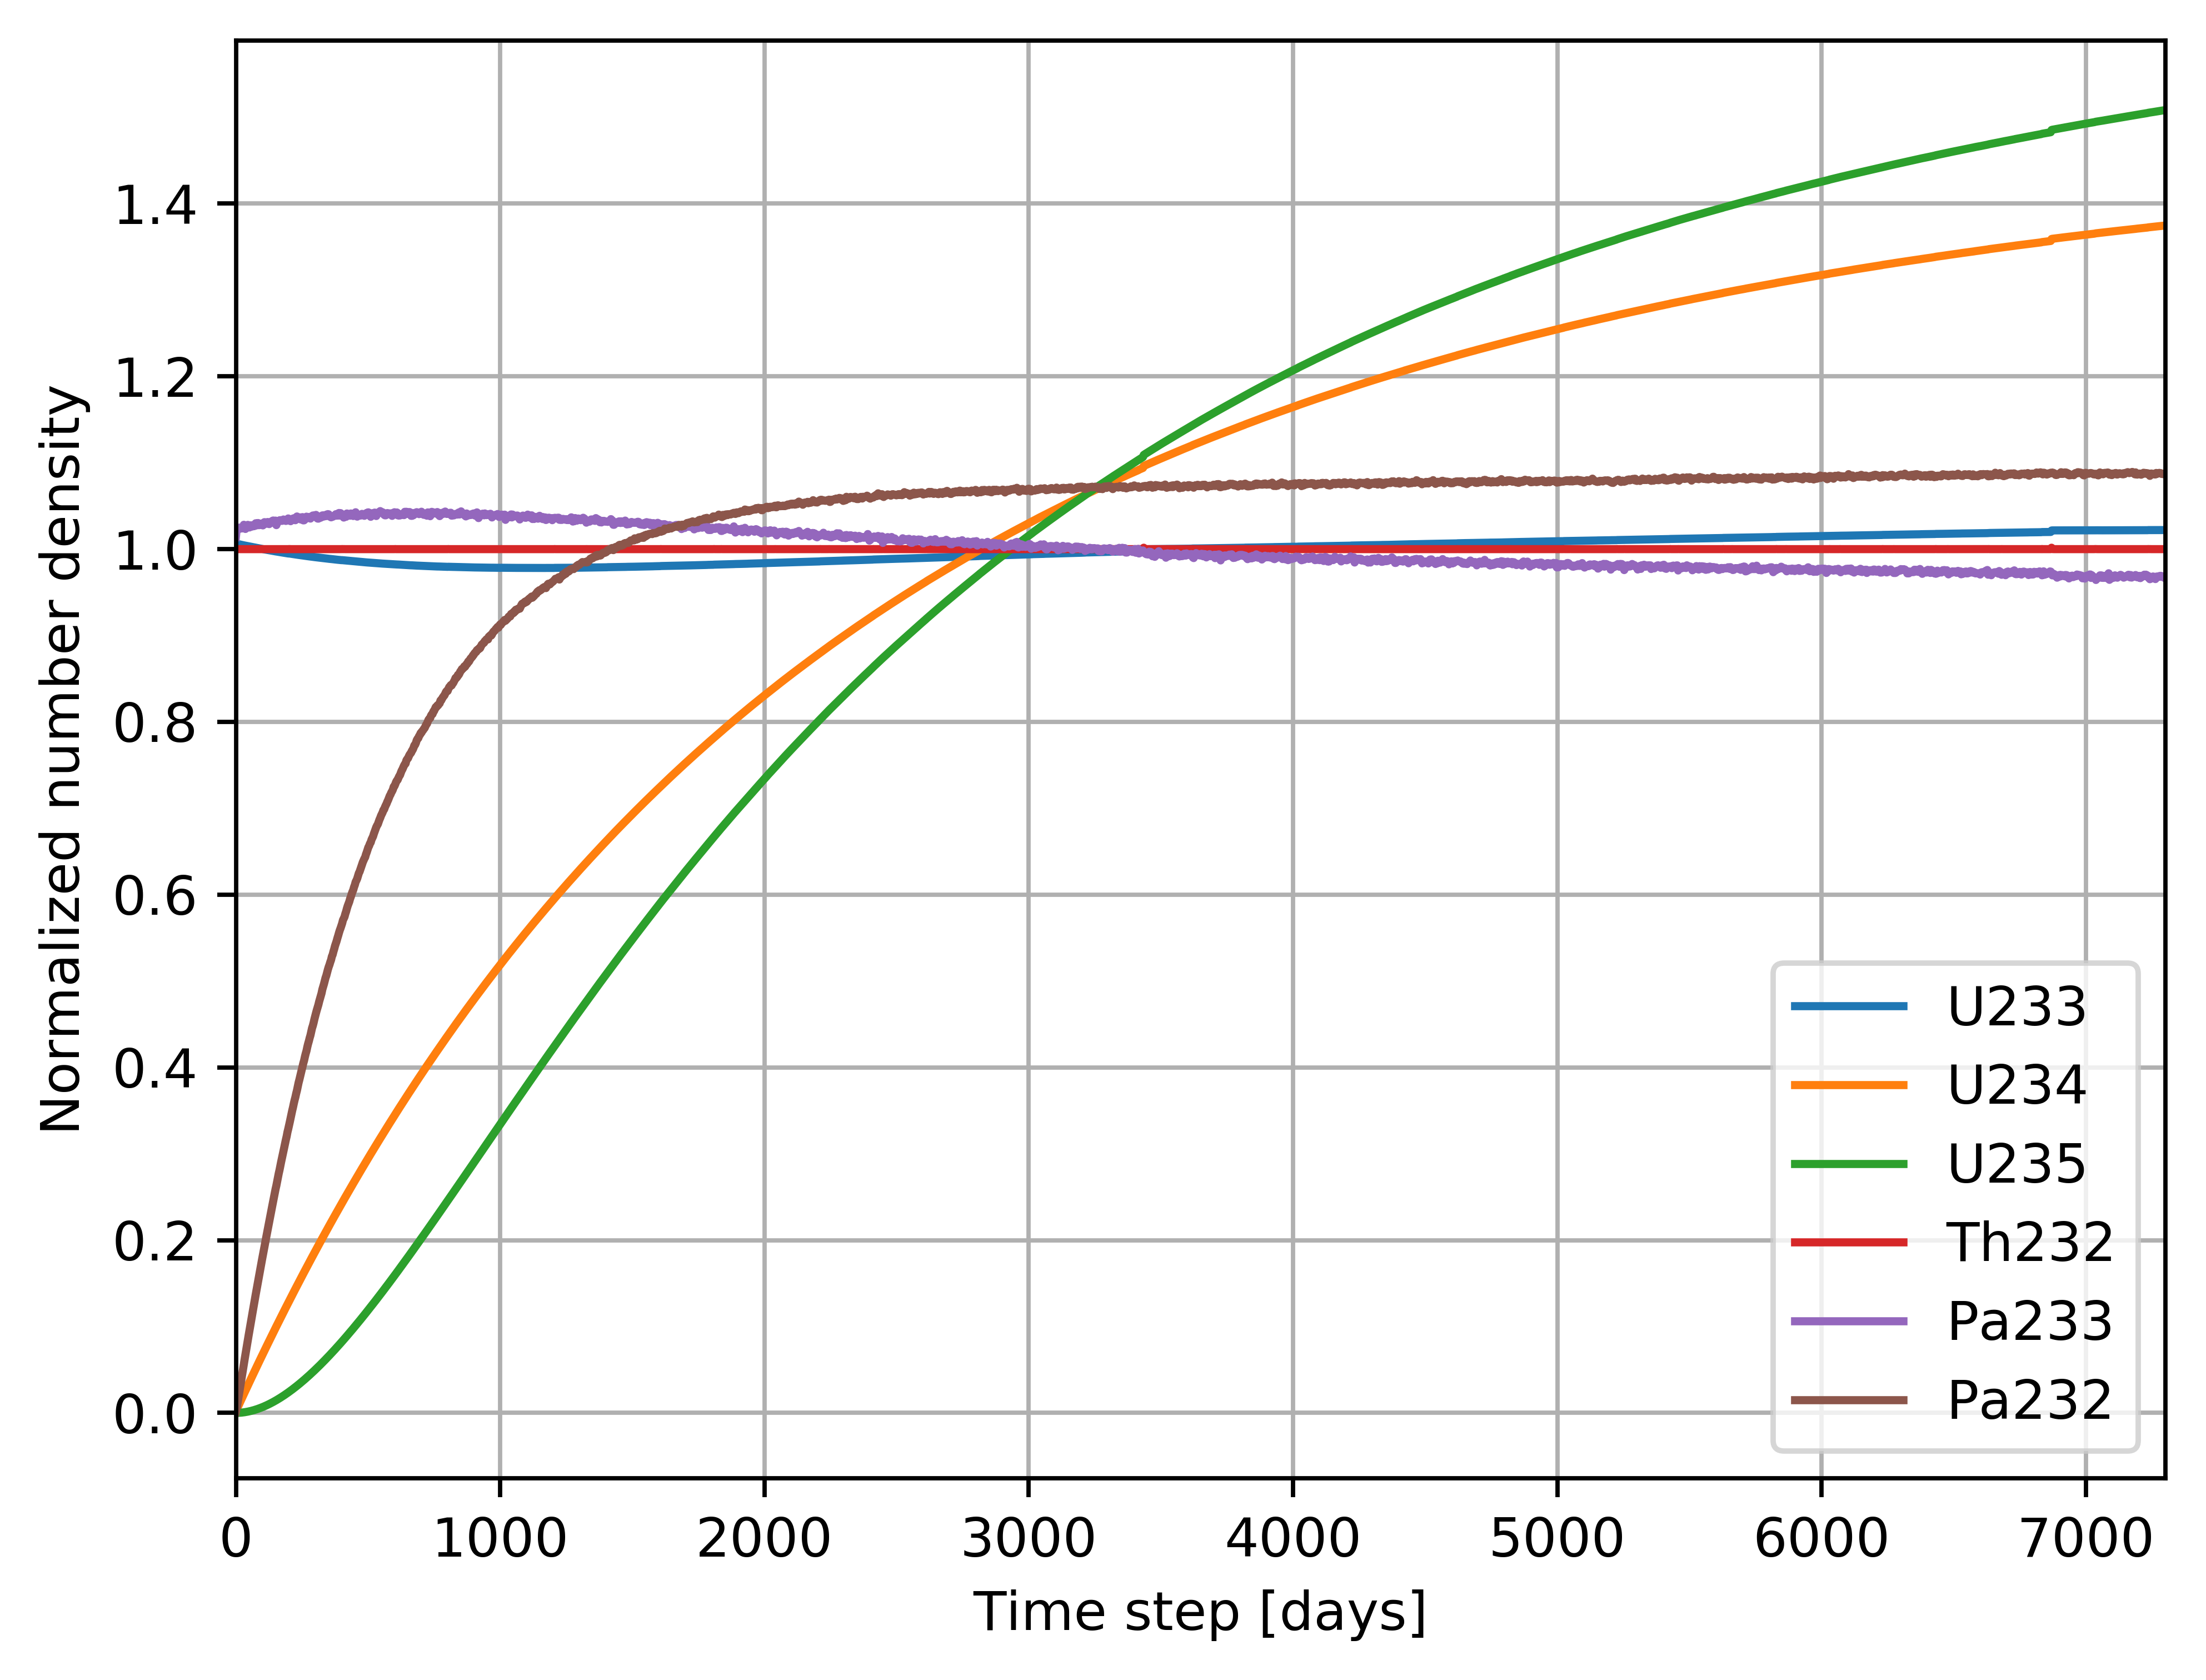
\includegraphics[width=\textwidth]{major_isotopes_adens.png}
  \caption{Number density of major nuclides during 60 years of reactor 
  operation.}
  \label{fig:adens_eq}
\end{figure}
In contrast, a wide variety of nuclides, including fissile isotopes (e.g. 
$^{235}$U) and non-fissile strong absorbers (e.g. $^{234}$U), kept accumulating 
in the core. Figure~\ref{fig:fissile_short} demonstrates production of fissile 
isotopes in the core. In the end of the considered operational time, the core 
contained significant $^{235}$U ($\approx10^{-5}$ atom/b-cm), $^{239}$Pu 
($\approx5\times10^{-7}$ atom/b-cm), and $^{241}$Pu ($\approx 5\times10^{-7}$ 
atom/b-cm). Meanwhile, the equilibrium number density of the target fissile 
isotope $^{233}$U was approximately 7.97$\times10^{-5}$ atom/b-cm. Thus, 
production of new fissile materials in the core, as well as $^{233}$U breeding, 
made it possible to compensate for negative effects of strong absorber 
accumulation and keep the reactor critical.
\begin{figure}[htp!] % replace 't' with 'b' to 
  \centering
  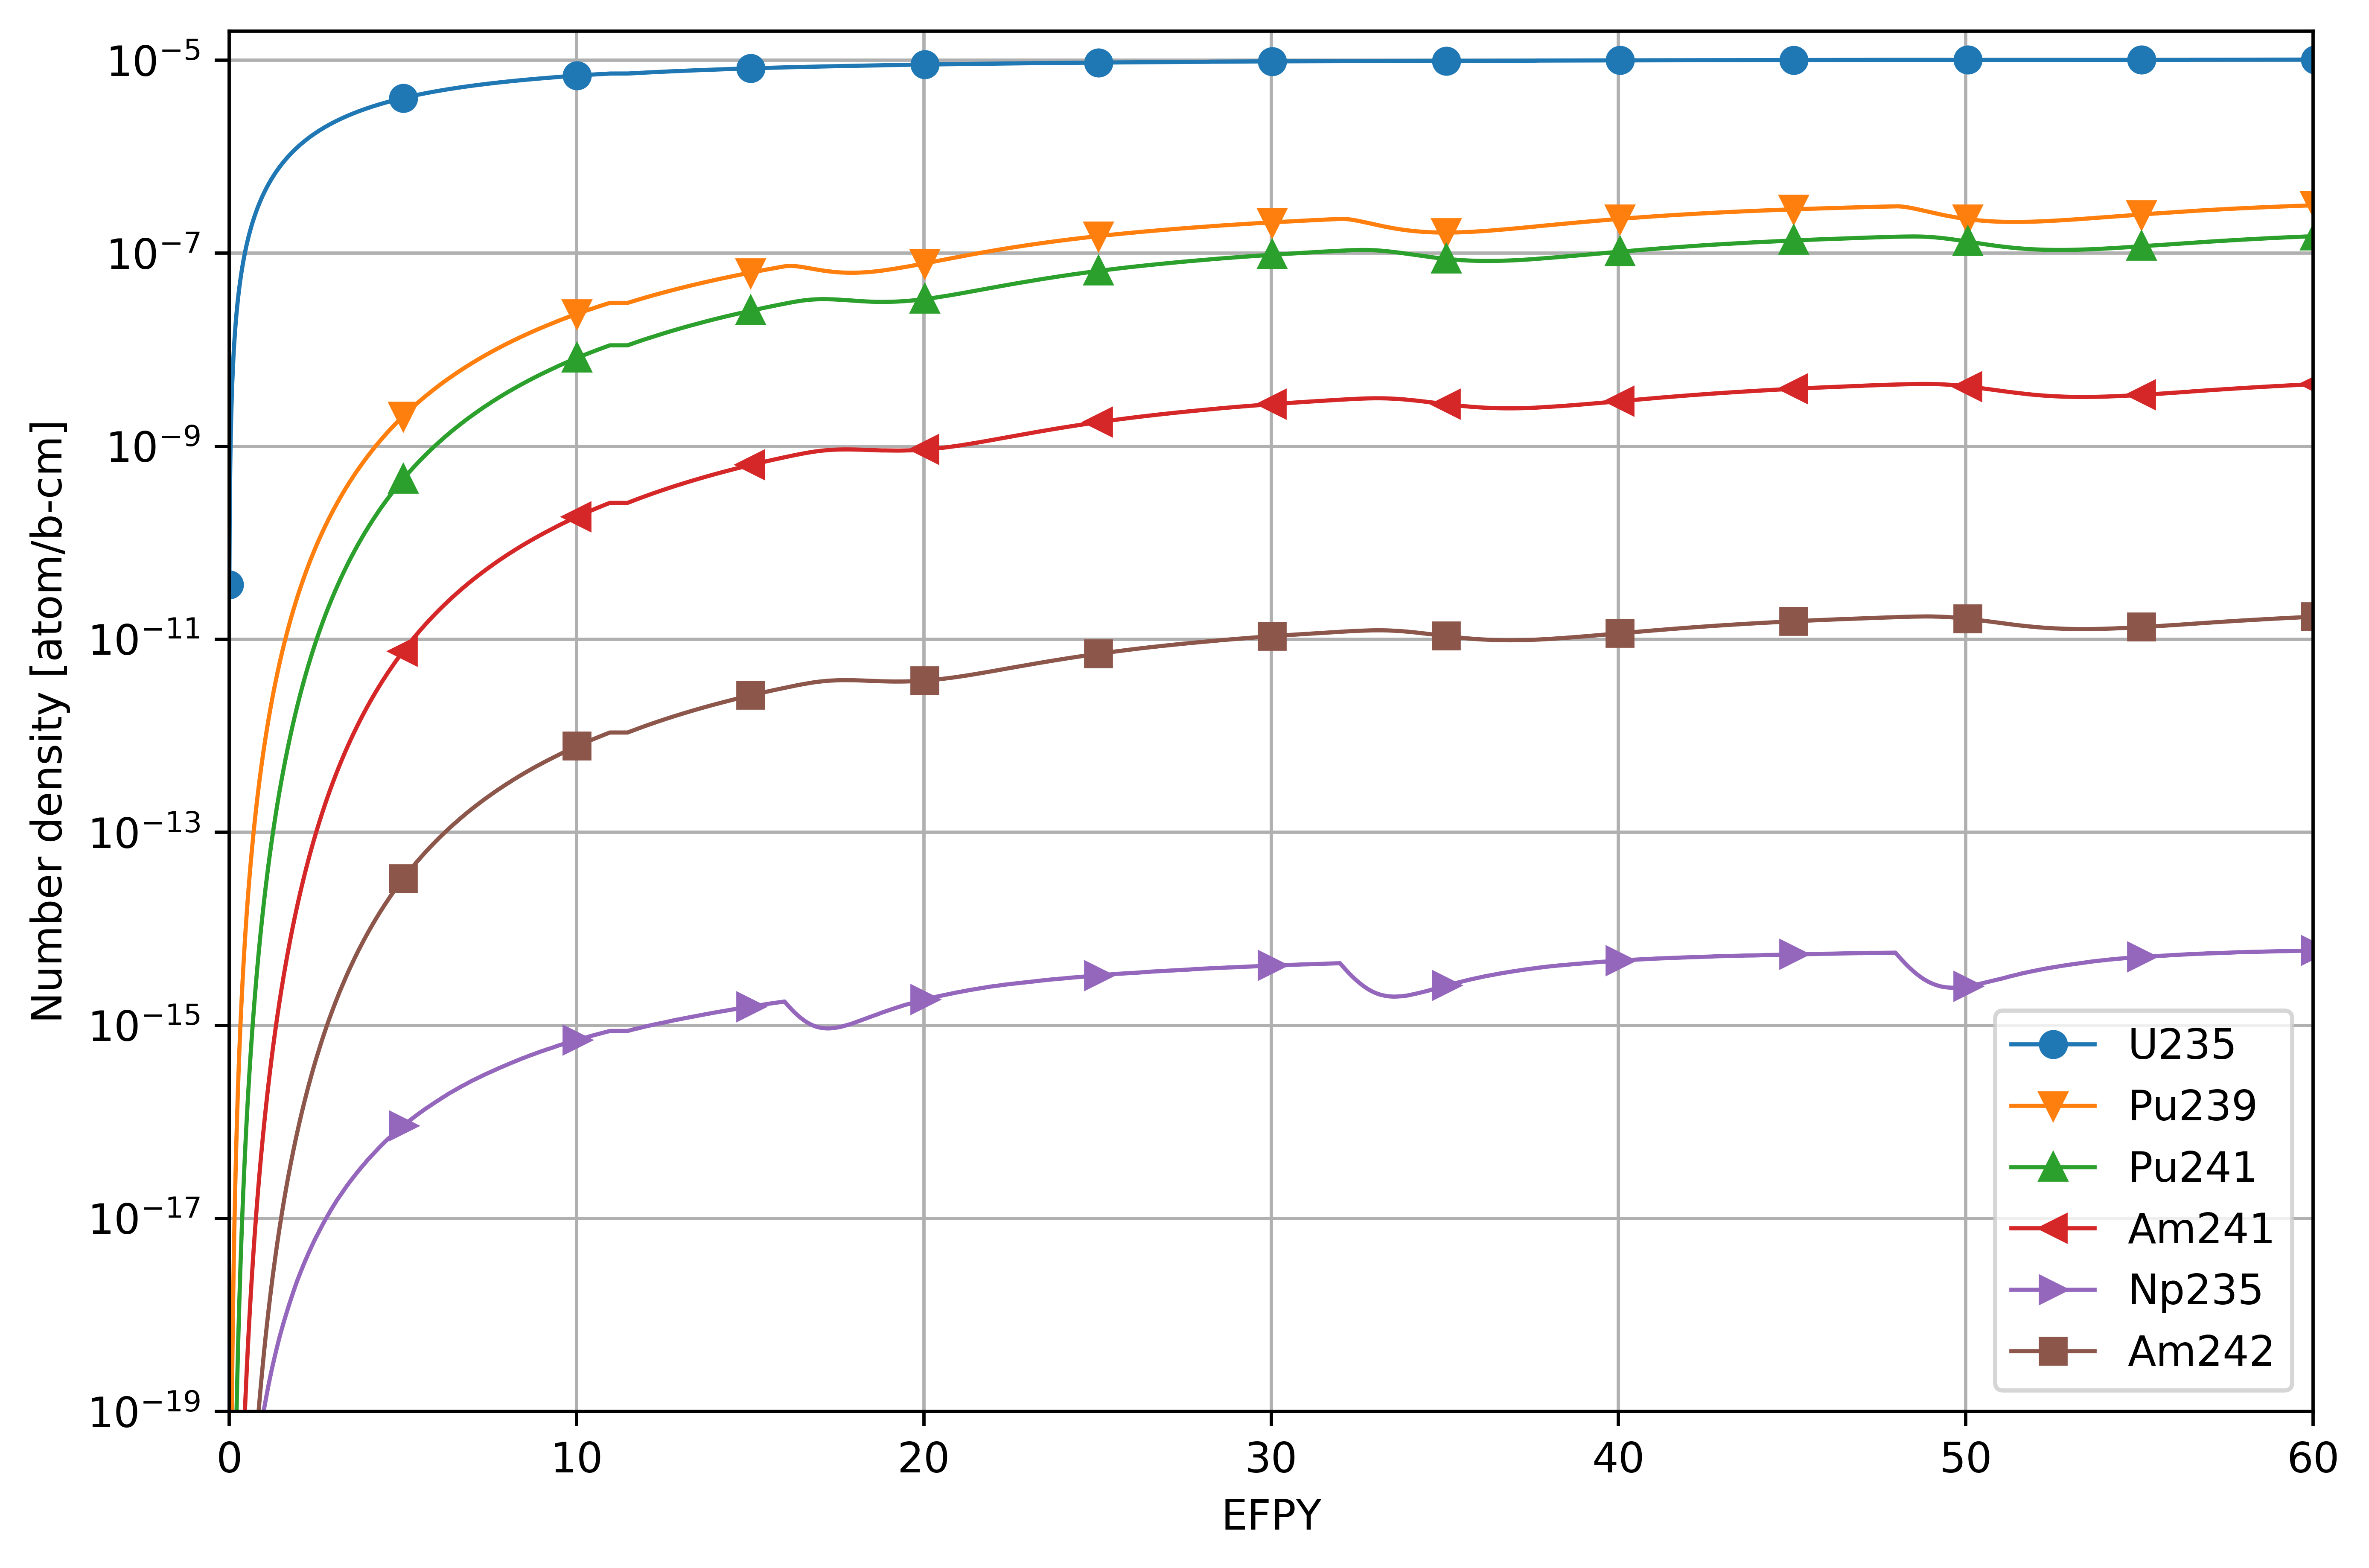
\includegraphics[width=\textwidth]{fissile_short.png}
  \caption{Number density of fissile in epithermal spectrum nuclides 
  accumulation during the reactor operation.}
  \label{fig:fissile_short}
\end{figure}

\subsection{Neutron spectrum}
Figure~\ref{fig:spectrum} shows the normalized neutron flux spectrum for the 
full-core \gls{MSBR} model in the energy range from $10^{-8}$ to $10$ MeV. The 
neutron energy spectrum at equilibrium is harder than at startup due to 
$^{238}$Pu, $^{239}$Pu, $^{240}$Pu, $^{241}$Pu, and $^{242}$Pu accumulation in 
the core during reactor operation.  
\begin{figure}[ht!] % replace 't' with 'b'         to force it to 
  \centering
  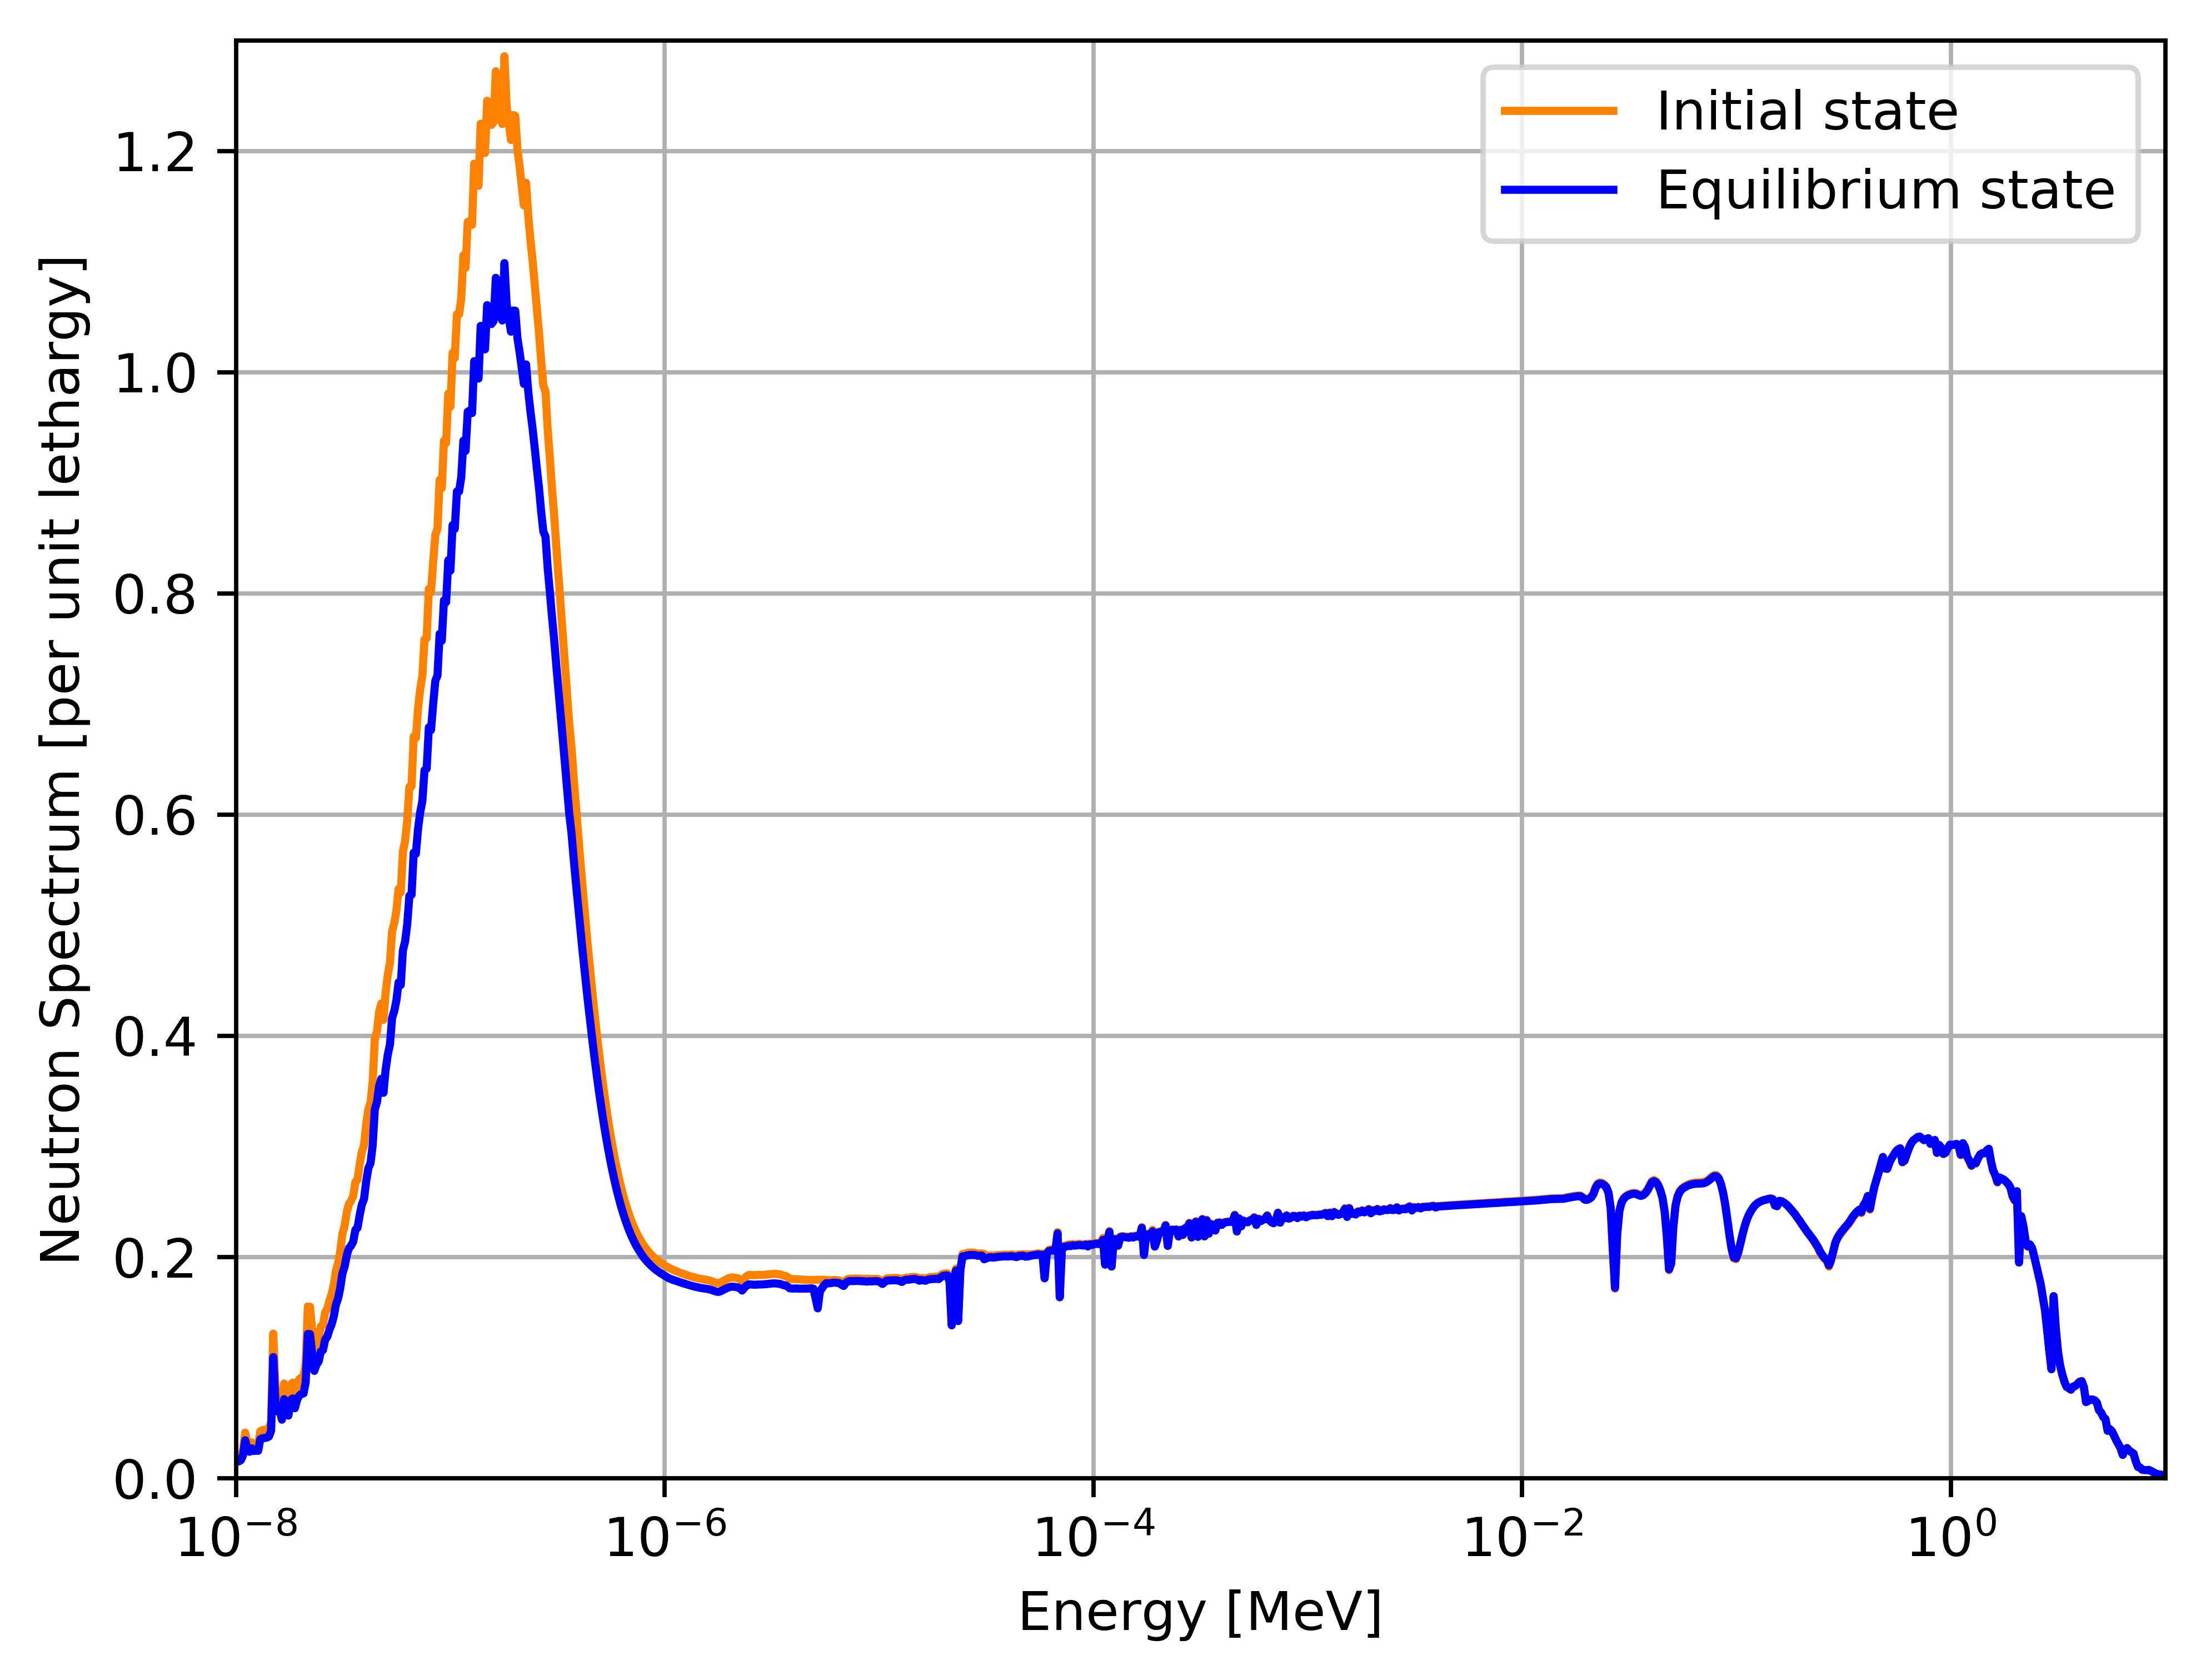
\includegraphics[width=\textwidth]{spectrum.png} \caption{Neutron flux energy 
  spectrum normalized by unit lethargy for initial and equilibrium fuel salt 
  composition.}
  \label{fig:spectrum}
\end{figure}

Figure~\ref{fig:spectrum_zones} shows that zone I produced more thermal neutrons 
than zone II, corresponding to a majority of fissions occurring in the central part 
of the core. In the undermoderated zone II, the neutron energy spectrum is harder, 
which leads to more neutrons capture by $^{232}$Th and helps achieve relatively 
high breeding ratio. Moreover, the (n,$\gamma$) resonance energy range in $^{232}$Th 
is from 10$^{-4}$ to 10$^{-2}$ MeV. Therefore, the moderator-to-fuel ratio for zone 
II was chosen to shift the neutron energy spectrum in this range. Furthermore, in the 
central core region (zone I), the neutron energy spectrum shifts to a harder spectrum 
over 20 years of reactor operation. Meanwhile, in the outer core region (zone II), a 
similar spectral shift takes place at a reduced scale. These results are in a good 
agreement with original ORNL report \cite{robertson_conceptual_1971} and the most recent 
whole-core steady-state study \cite{park_whole_2015}.

It is important to obtain the epithermal and thermal spectra to produce $^{233}$U from 
$^{232}$Th because the radiative capture cross section of thorium decreases monotonically 
from $10^{-10}$ MeV to $10^{-5}$ MeV. Hardening the spectrum tends to significantly 
increase resonance absorption in thorium and decrease absorptions in fissile and 
construction materials. 
\begin{figure}[ht!] % replace 't' with 'b' to force it to 
  \centering
  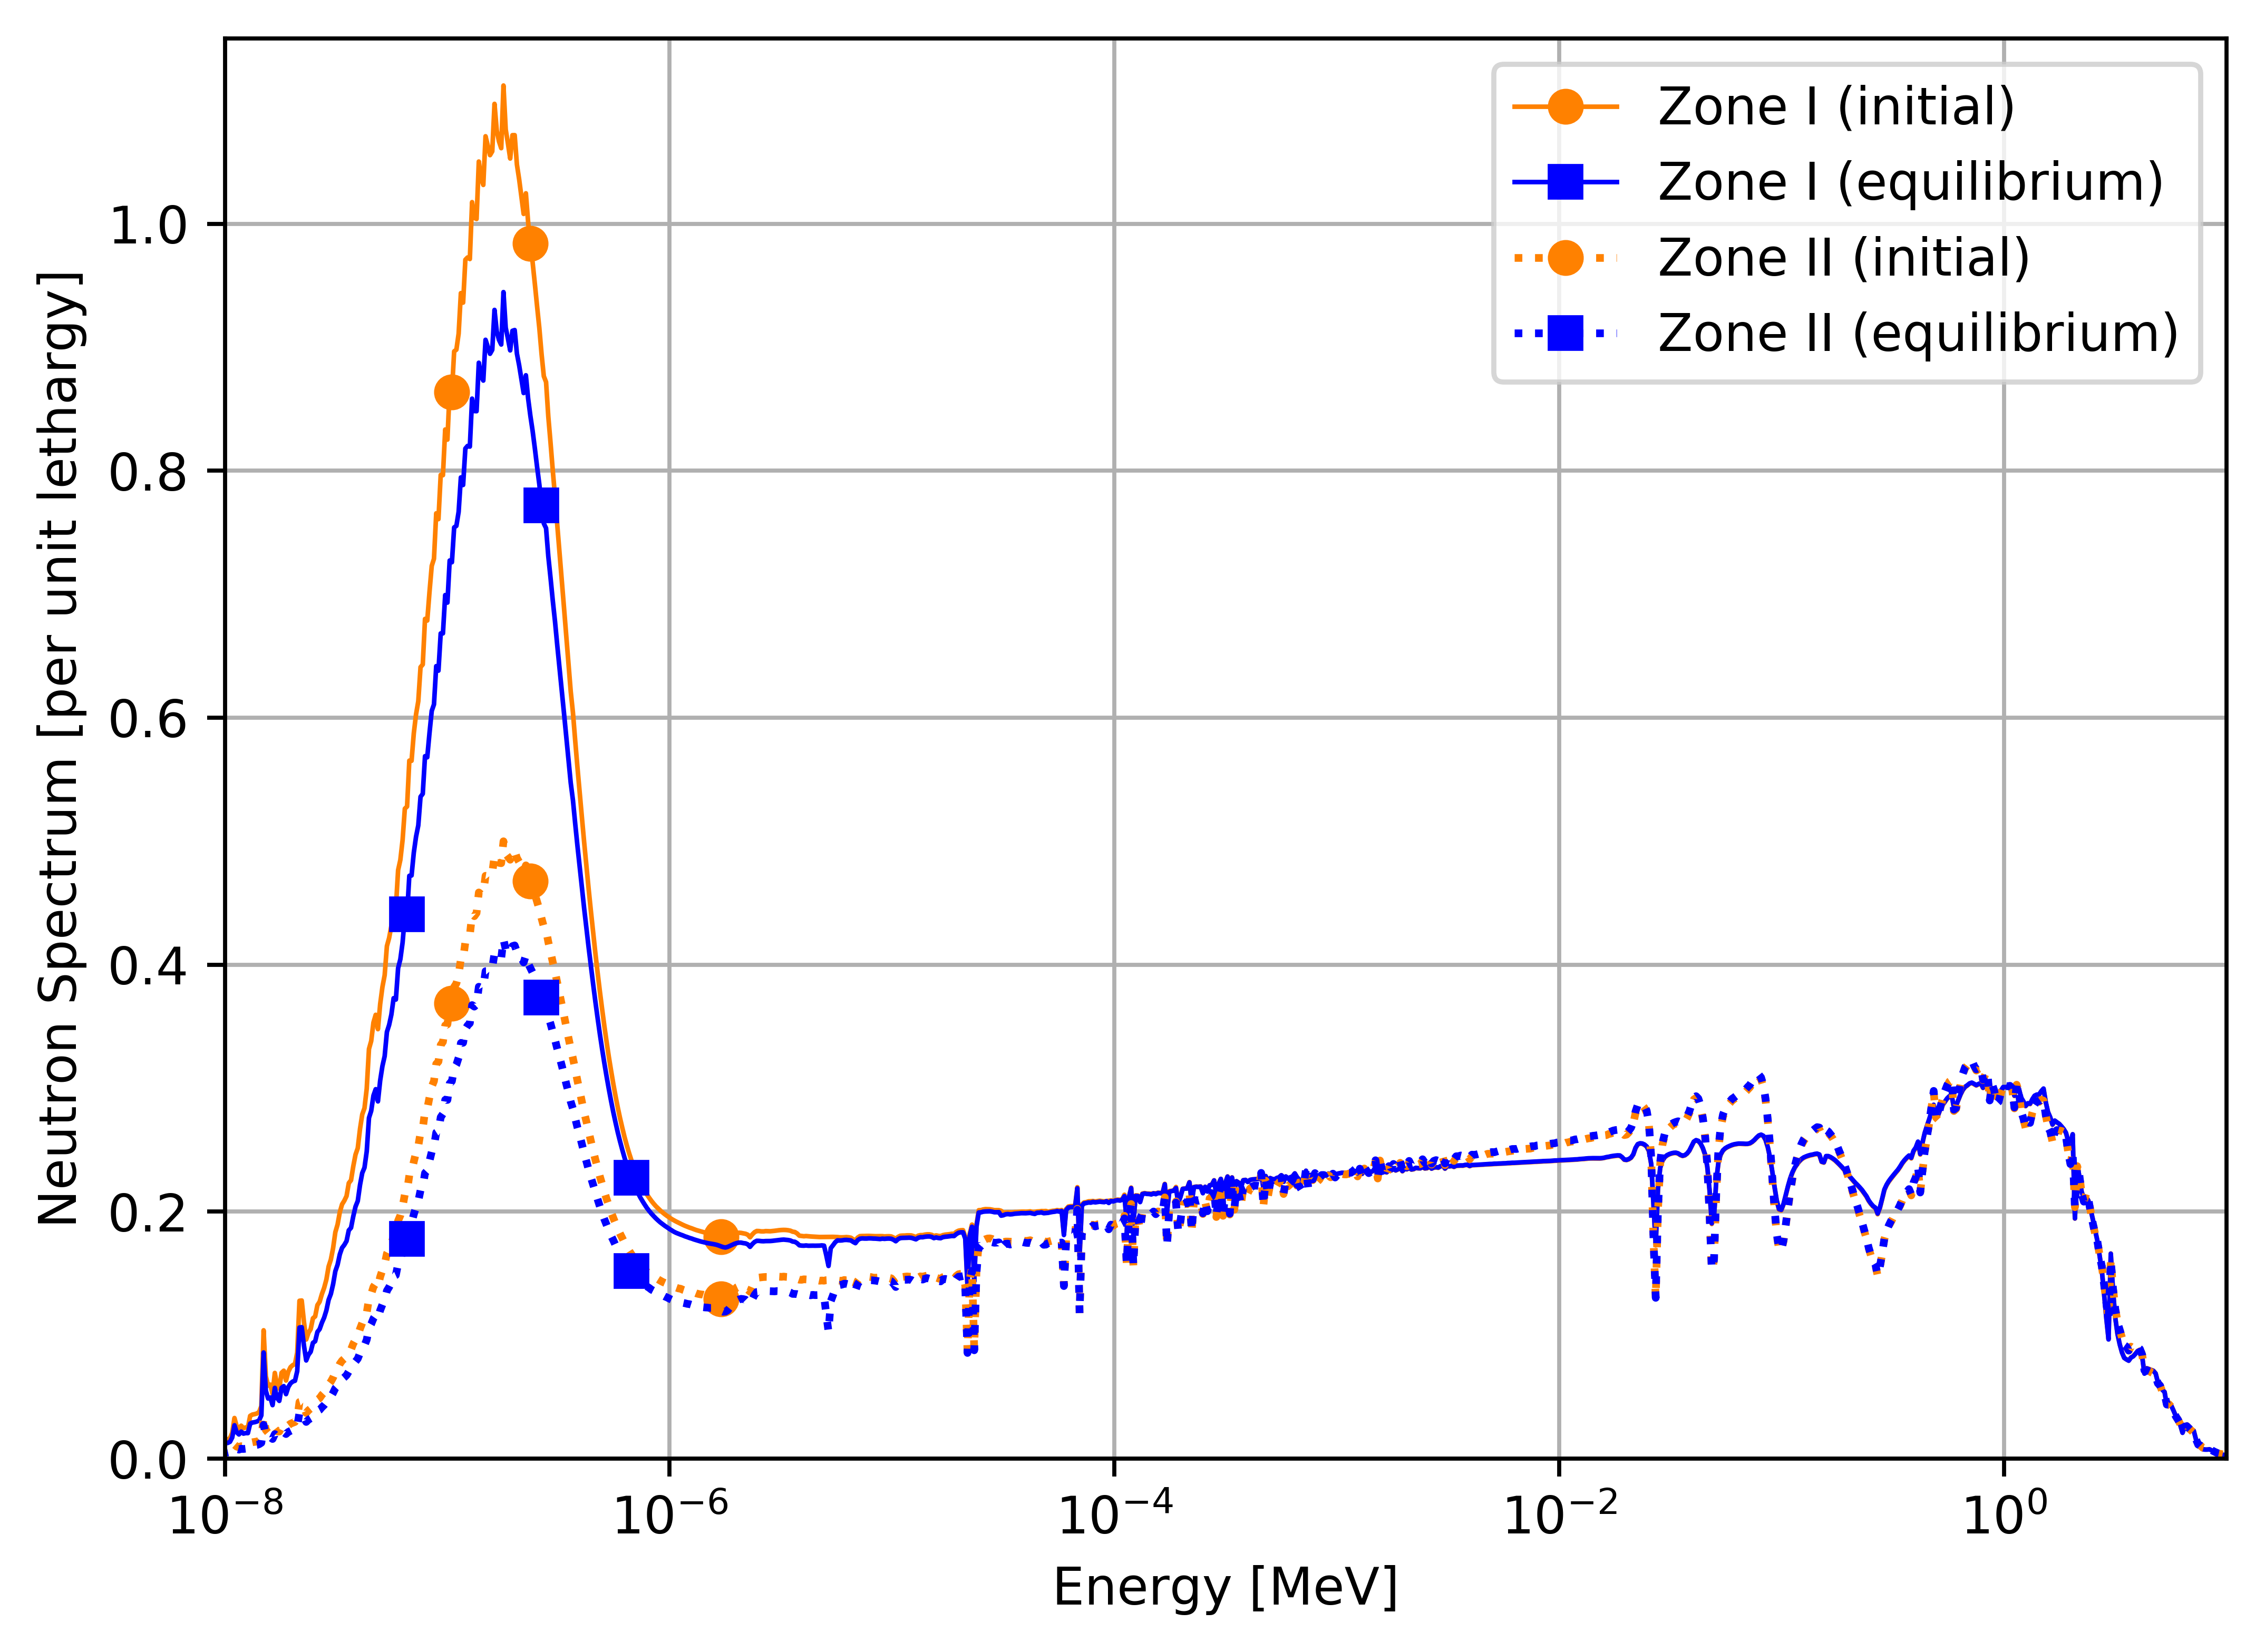
\includegraphics[width=\textwidth]{spectrum_zones.png} 
  \caption{Neutron flux energy spectrum in different core regions normalized by 
unit lethargy for the initial and equilibrium fuel salt composition.}
  \label{fig:spectrum_zones}
\end{figure}

\subsection{Neutron flux}
Figure~\ref{fig:radial_flux} shows the radial distribution of fast and thermal 
neutron flux for the both initial and equilibrium composition. The neutron fluxes
have similar shapes for both compositions but the equilibrium case has a harder 
spectrum. A significant spectral shift was observed in the central region of 
the core (zone I), while for the outer region (zone II), it is negligible for fast 
but notable for thermal neutrons. These neutron flux radial distributions 
agree with the fluxes in the original ORNL report \cite{robertson_conceptual_1971}. 
Overall, spectrum hardening during \gls{MSBR} operation should be carefully 
studied when designing the reactivity control system.
\begin{figure}[ht!] % replace 't' with 'b' to force it to \centering
  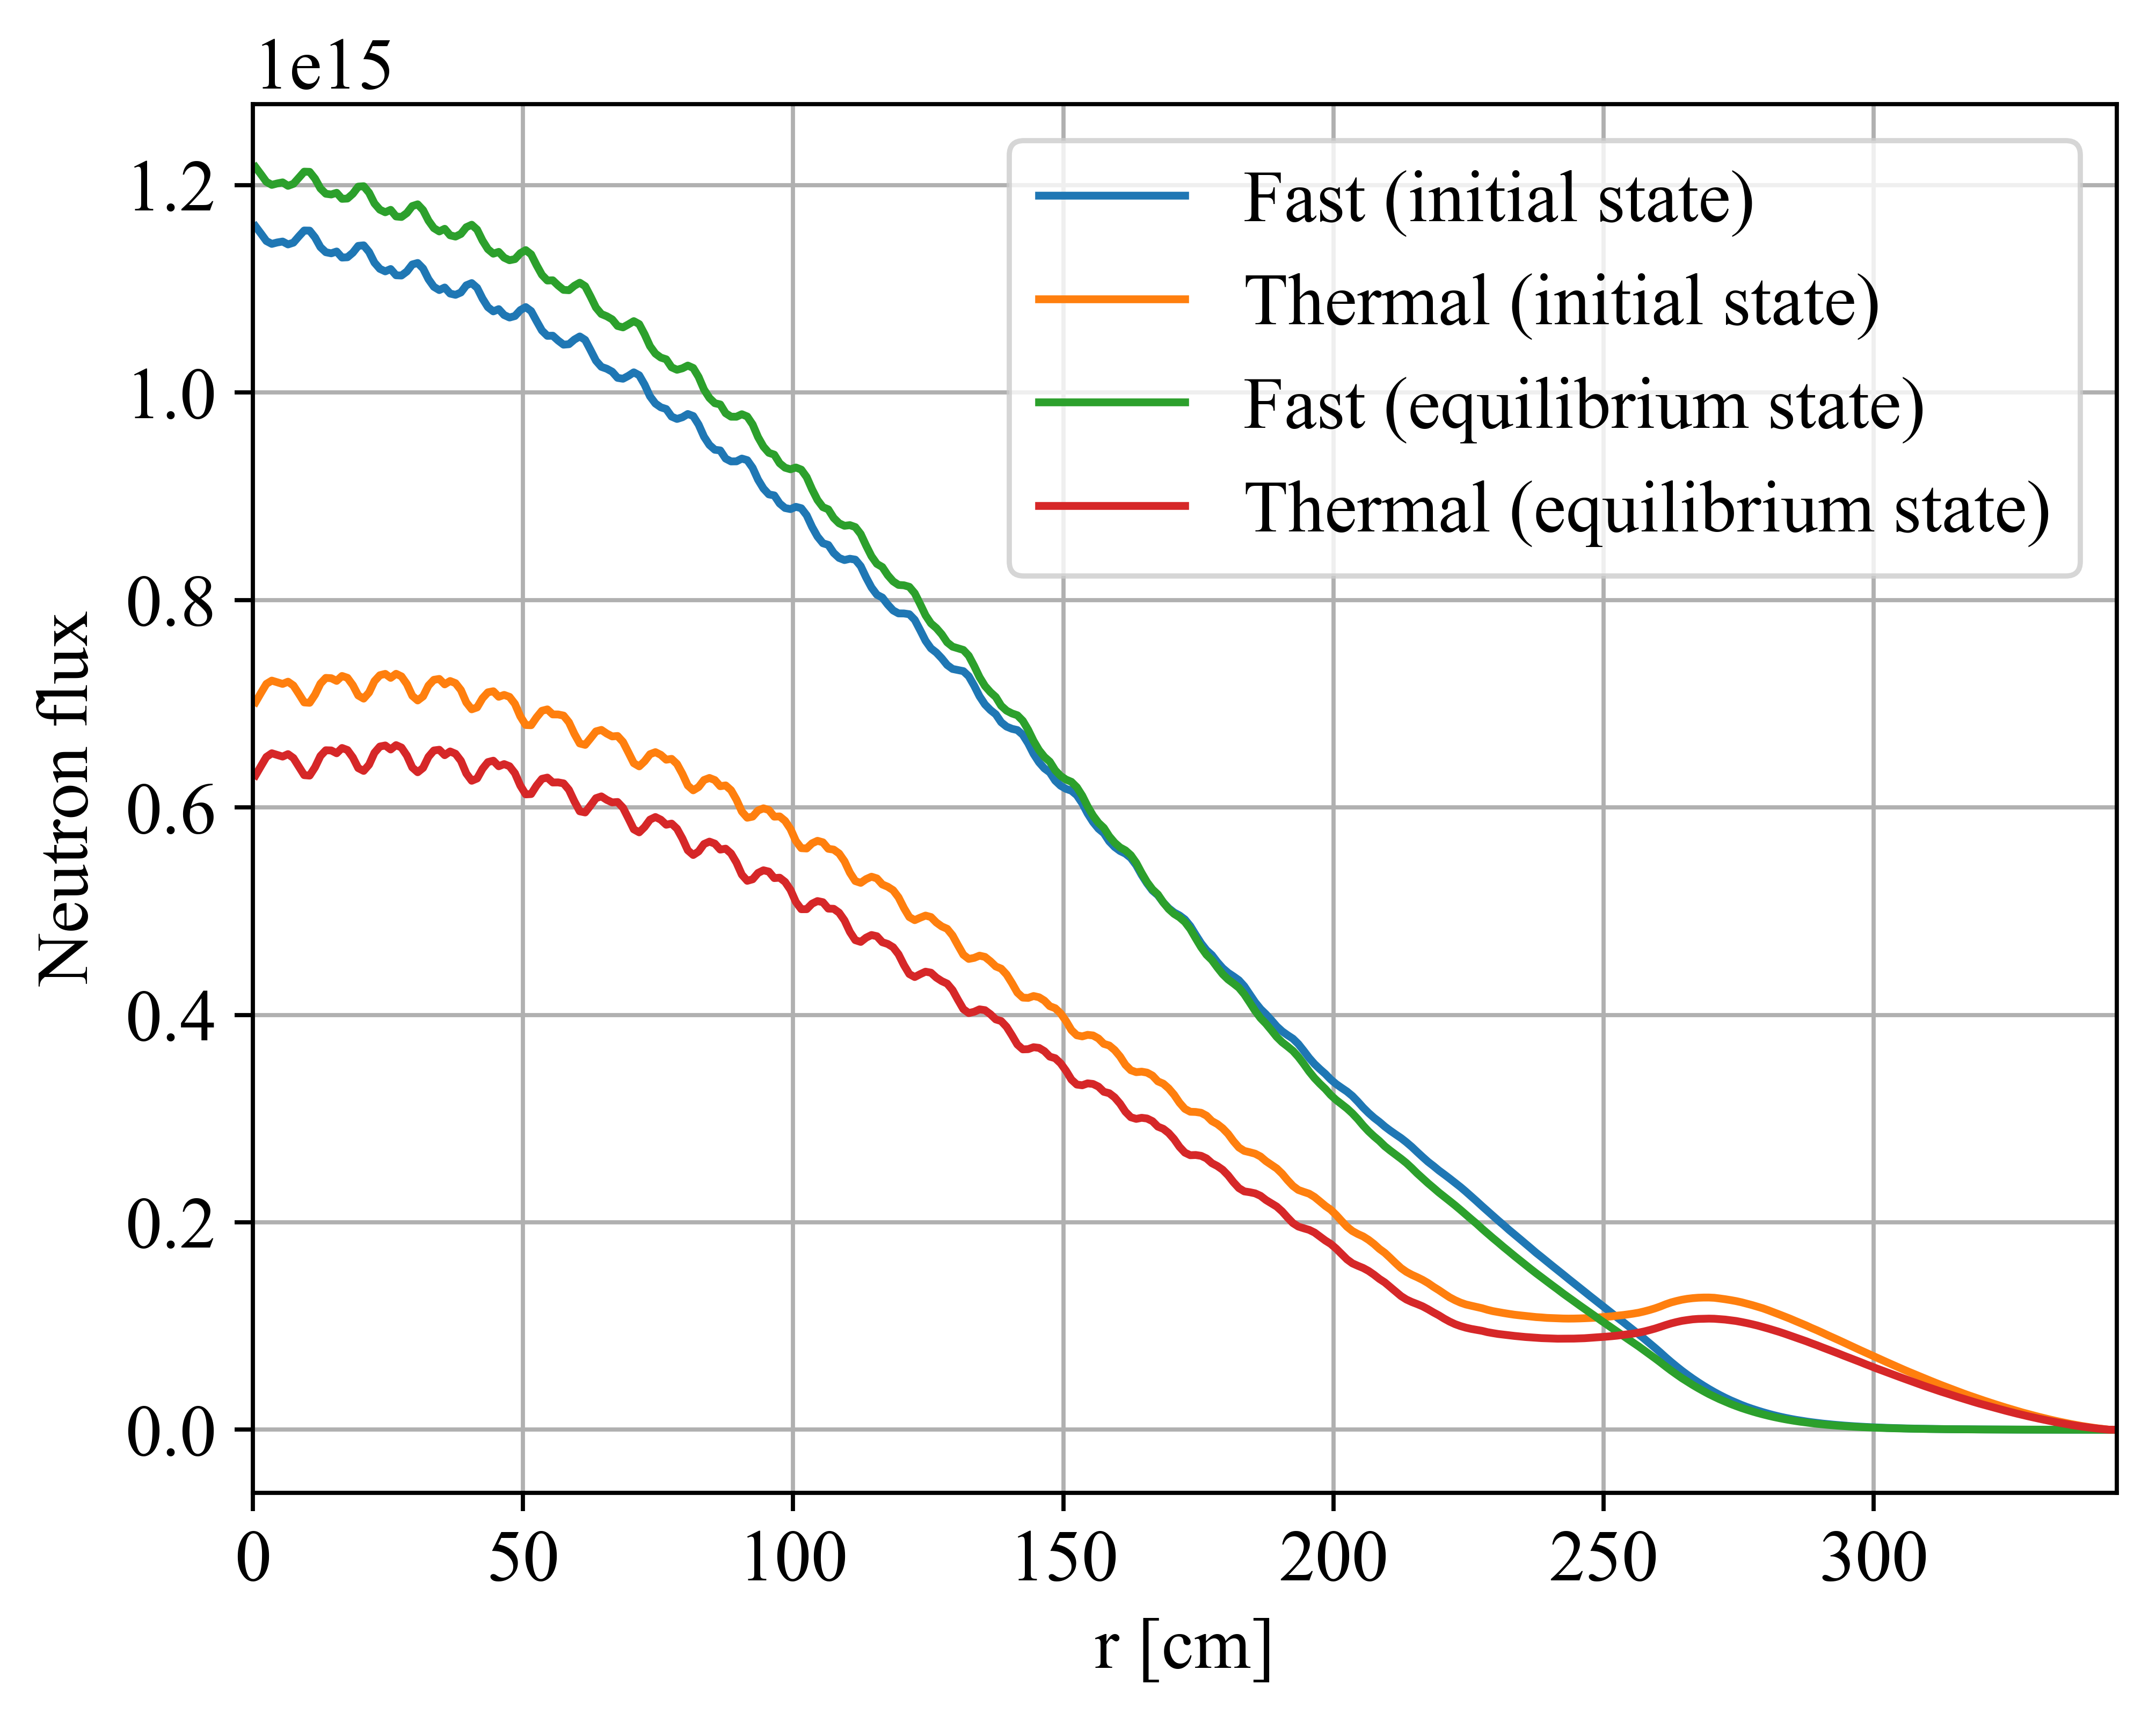
\includegraphics[width=\textwidth]{radial_flux.png} \caption{Radial neutron 
  flux distribution for initial and equilibrium fuel salt composition.}
  \label{fig:radial_flux}
\end{figure}

\subsection{Power and breeding distribution}
Table~\ref{tab:powgen_fraction}	 shows the power fraction in each zone for 
initial and equilibrium fuel compositions. Figure~\ref{fig:pow_den} reflects the 
normalized power distribution of the \gls{MSBR} quarter core, which is the same 
at both the initial and equilibrium states. For both the initial and equilibrium compositions, fission 
primarily occurs in the center of the core, namely zone I. The spectral shift 
during reactor operation results in different power fractions at startup and 
equilibrium, but most of the power is still generated in zone I at equilibrium. 
%%%%%%%%%%%%%%%%%%%%%%%%%%%%%%%%%%%%%%%%
\begin{table}[ht!]
  \centering
  \caption{Power generation fraction in each zone for initial and equilibrium 
  state.}
\begin{tabularx}{\textwidth}{ m | s | s } \hline
Core region      & Initial      & Equilibrium   \\   \hline
Zone I           & 97.91\%      & 98.12\%   \\
Zone II          & 2.09\%       & 1.88\%   \\ \hline
\end{tabularx}
  \label{tab:powgen_fraction}
\end{table}
%%%%%%%%%%%%%%%%%%%%%%%%%%%%%%%%%%%%%%%%%%%%%%%%%%%%%%%%%%%%%%%%%%%%%%%%%%%%%%%%
Figure~\ref{fig:breeding_den} shows the neutron capture reaction rate 
distribution for $^{232}$Th normalized by the total neutron flux for initial 
and equilibrium states. The distribution reflects the spatial distribution of 
$^{233}$Th production in the core. The thorium-232 then $\beta$-decays to 
$^{233}$Pa, which is the precursor for $^{233}$U production. Accordingly, this 
characteristic represents the breeding distribution in the \gls{MSBR} core. 
Spectral shift does not cause significant changes in power nor in breeding 
distribution. Even after 20 years of operation, most of the power is still 
generated in zone I and the majority of $^{233}$Th is 
produced in zone II.
\begin{figure}[ht!] % replace 't' with 'b' to force it to \centering
  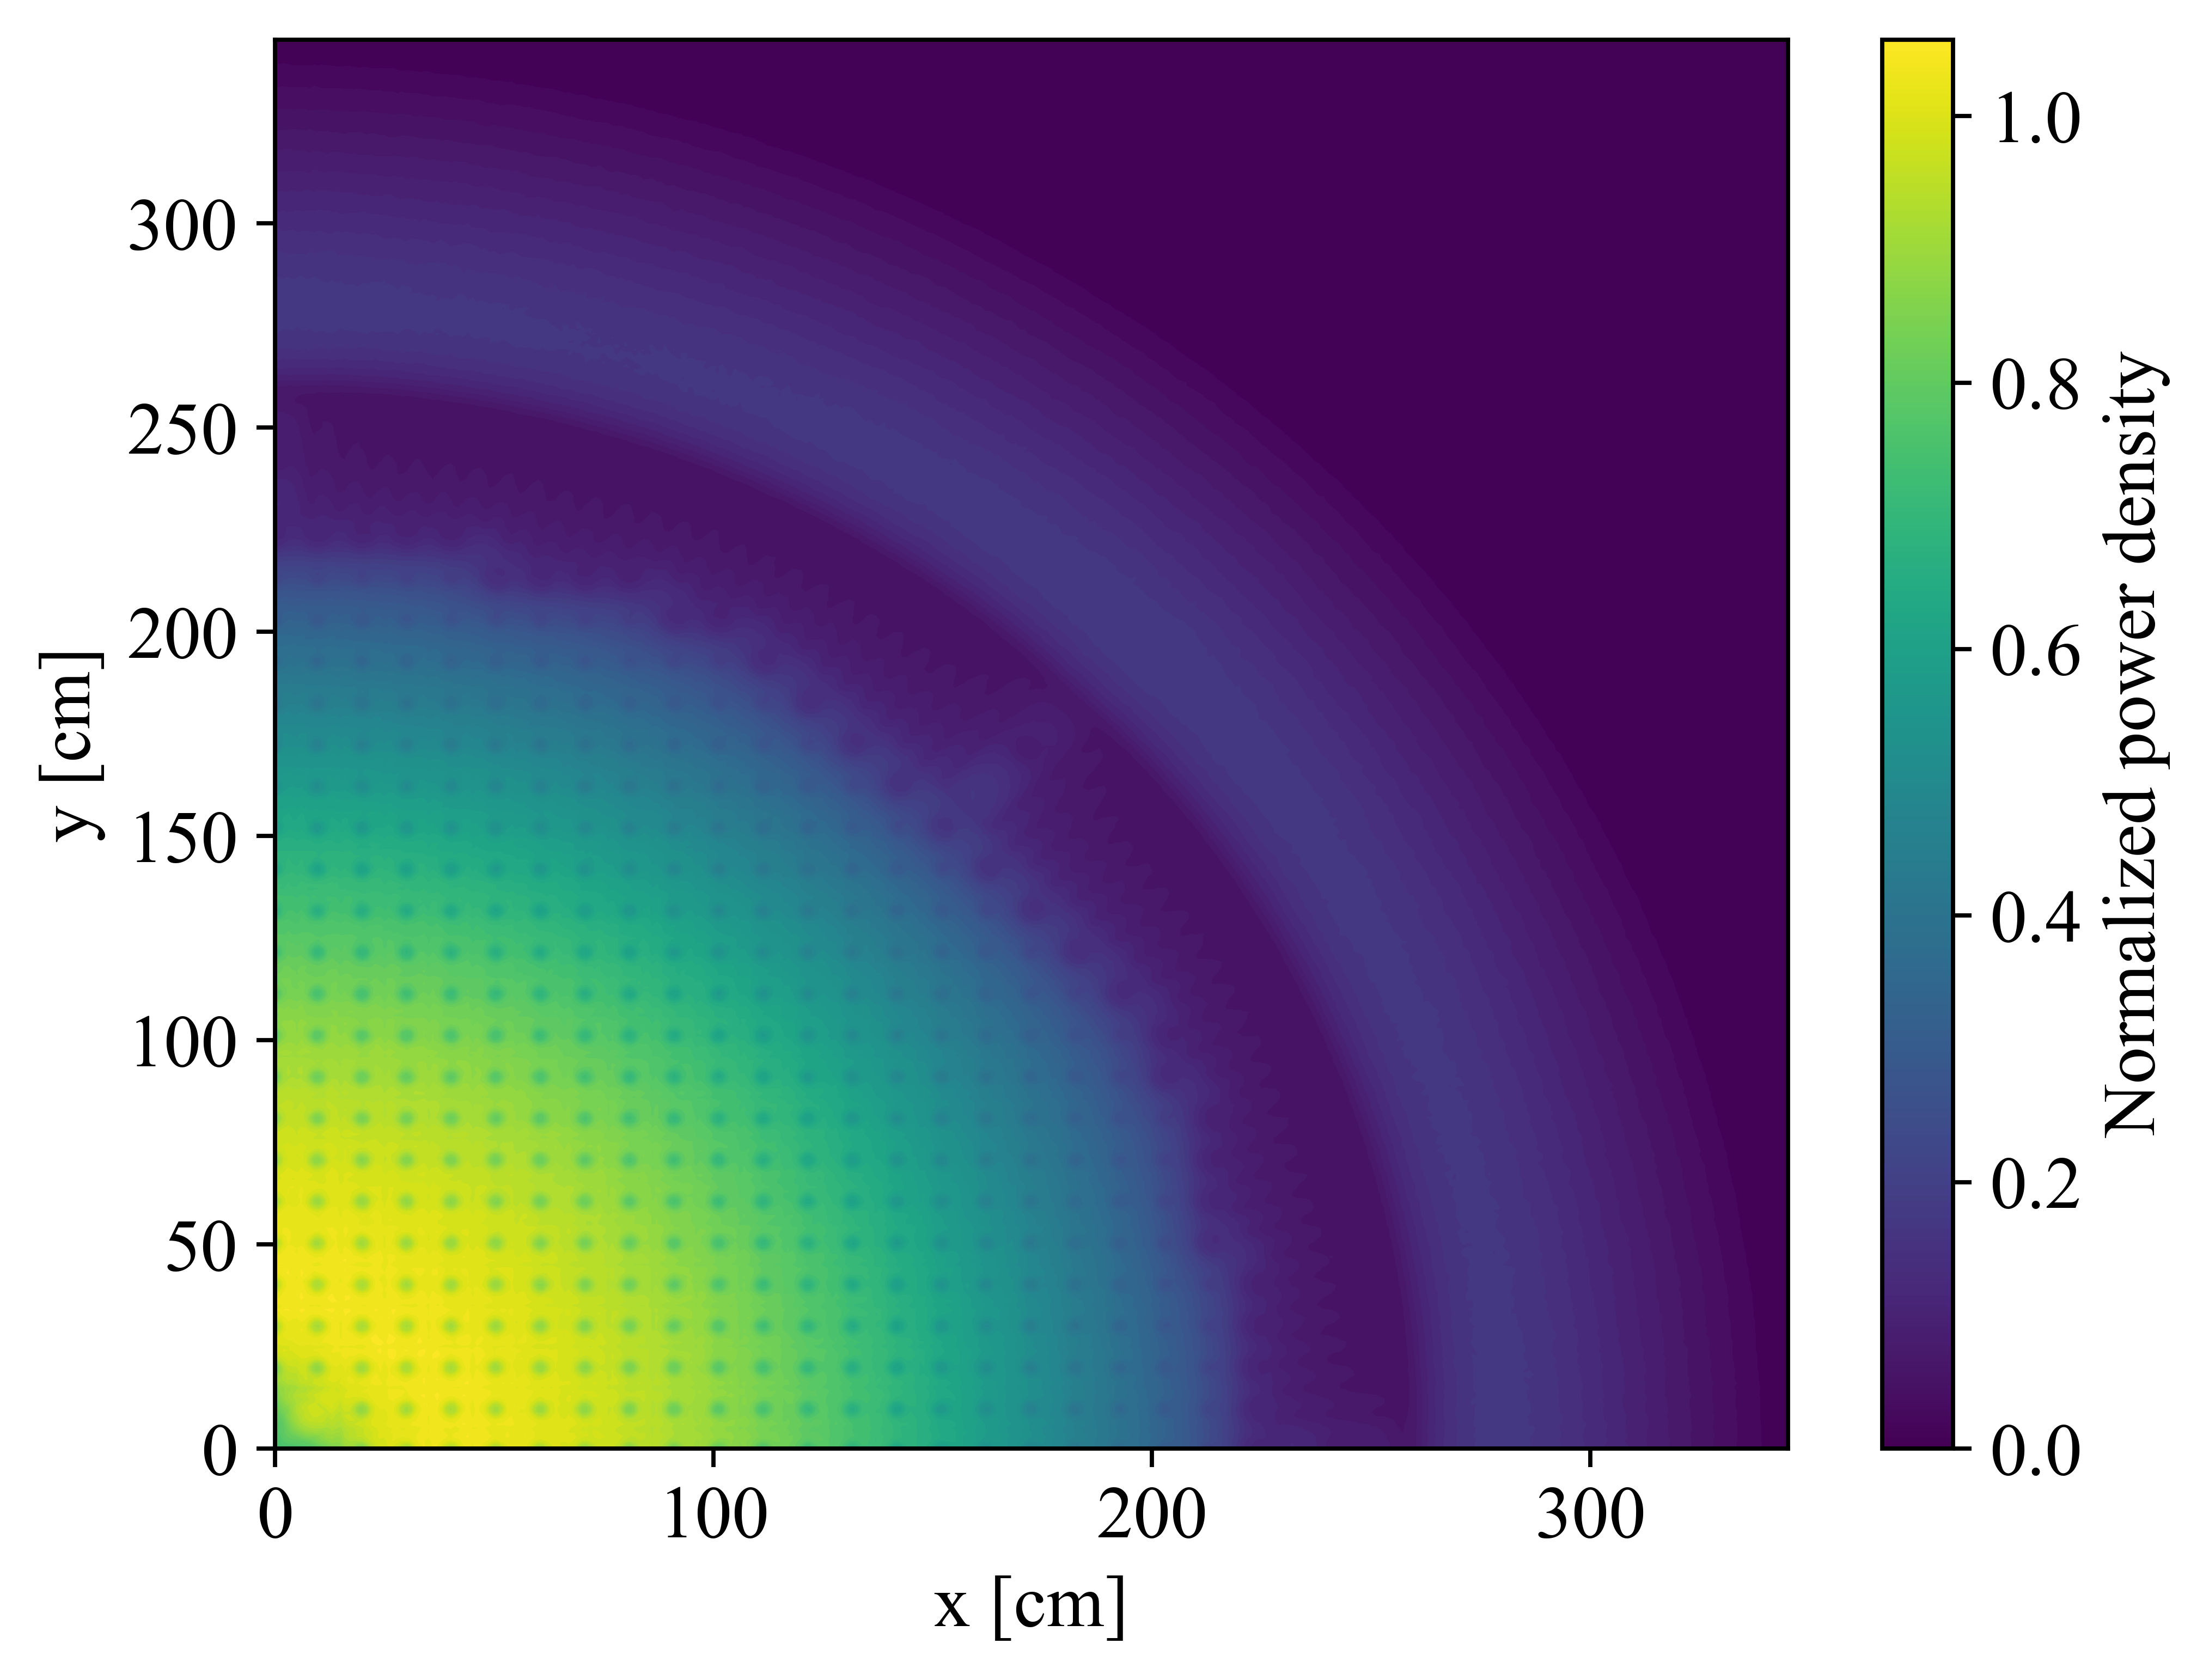
\includegraphics[width=\textwidth]{power_distribution_eq.png} 
  \caption{Normalized power density for equilibrium fuel salt 
  composition.}
  \label{fig:pow_den}
\end{figure}
\begin{figure}[ht!] % replace 't' with 'b' to force it to \centering
  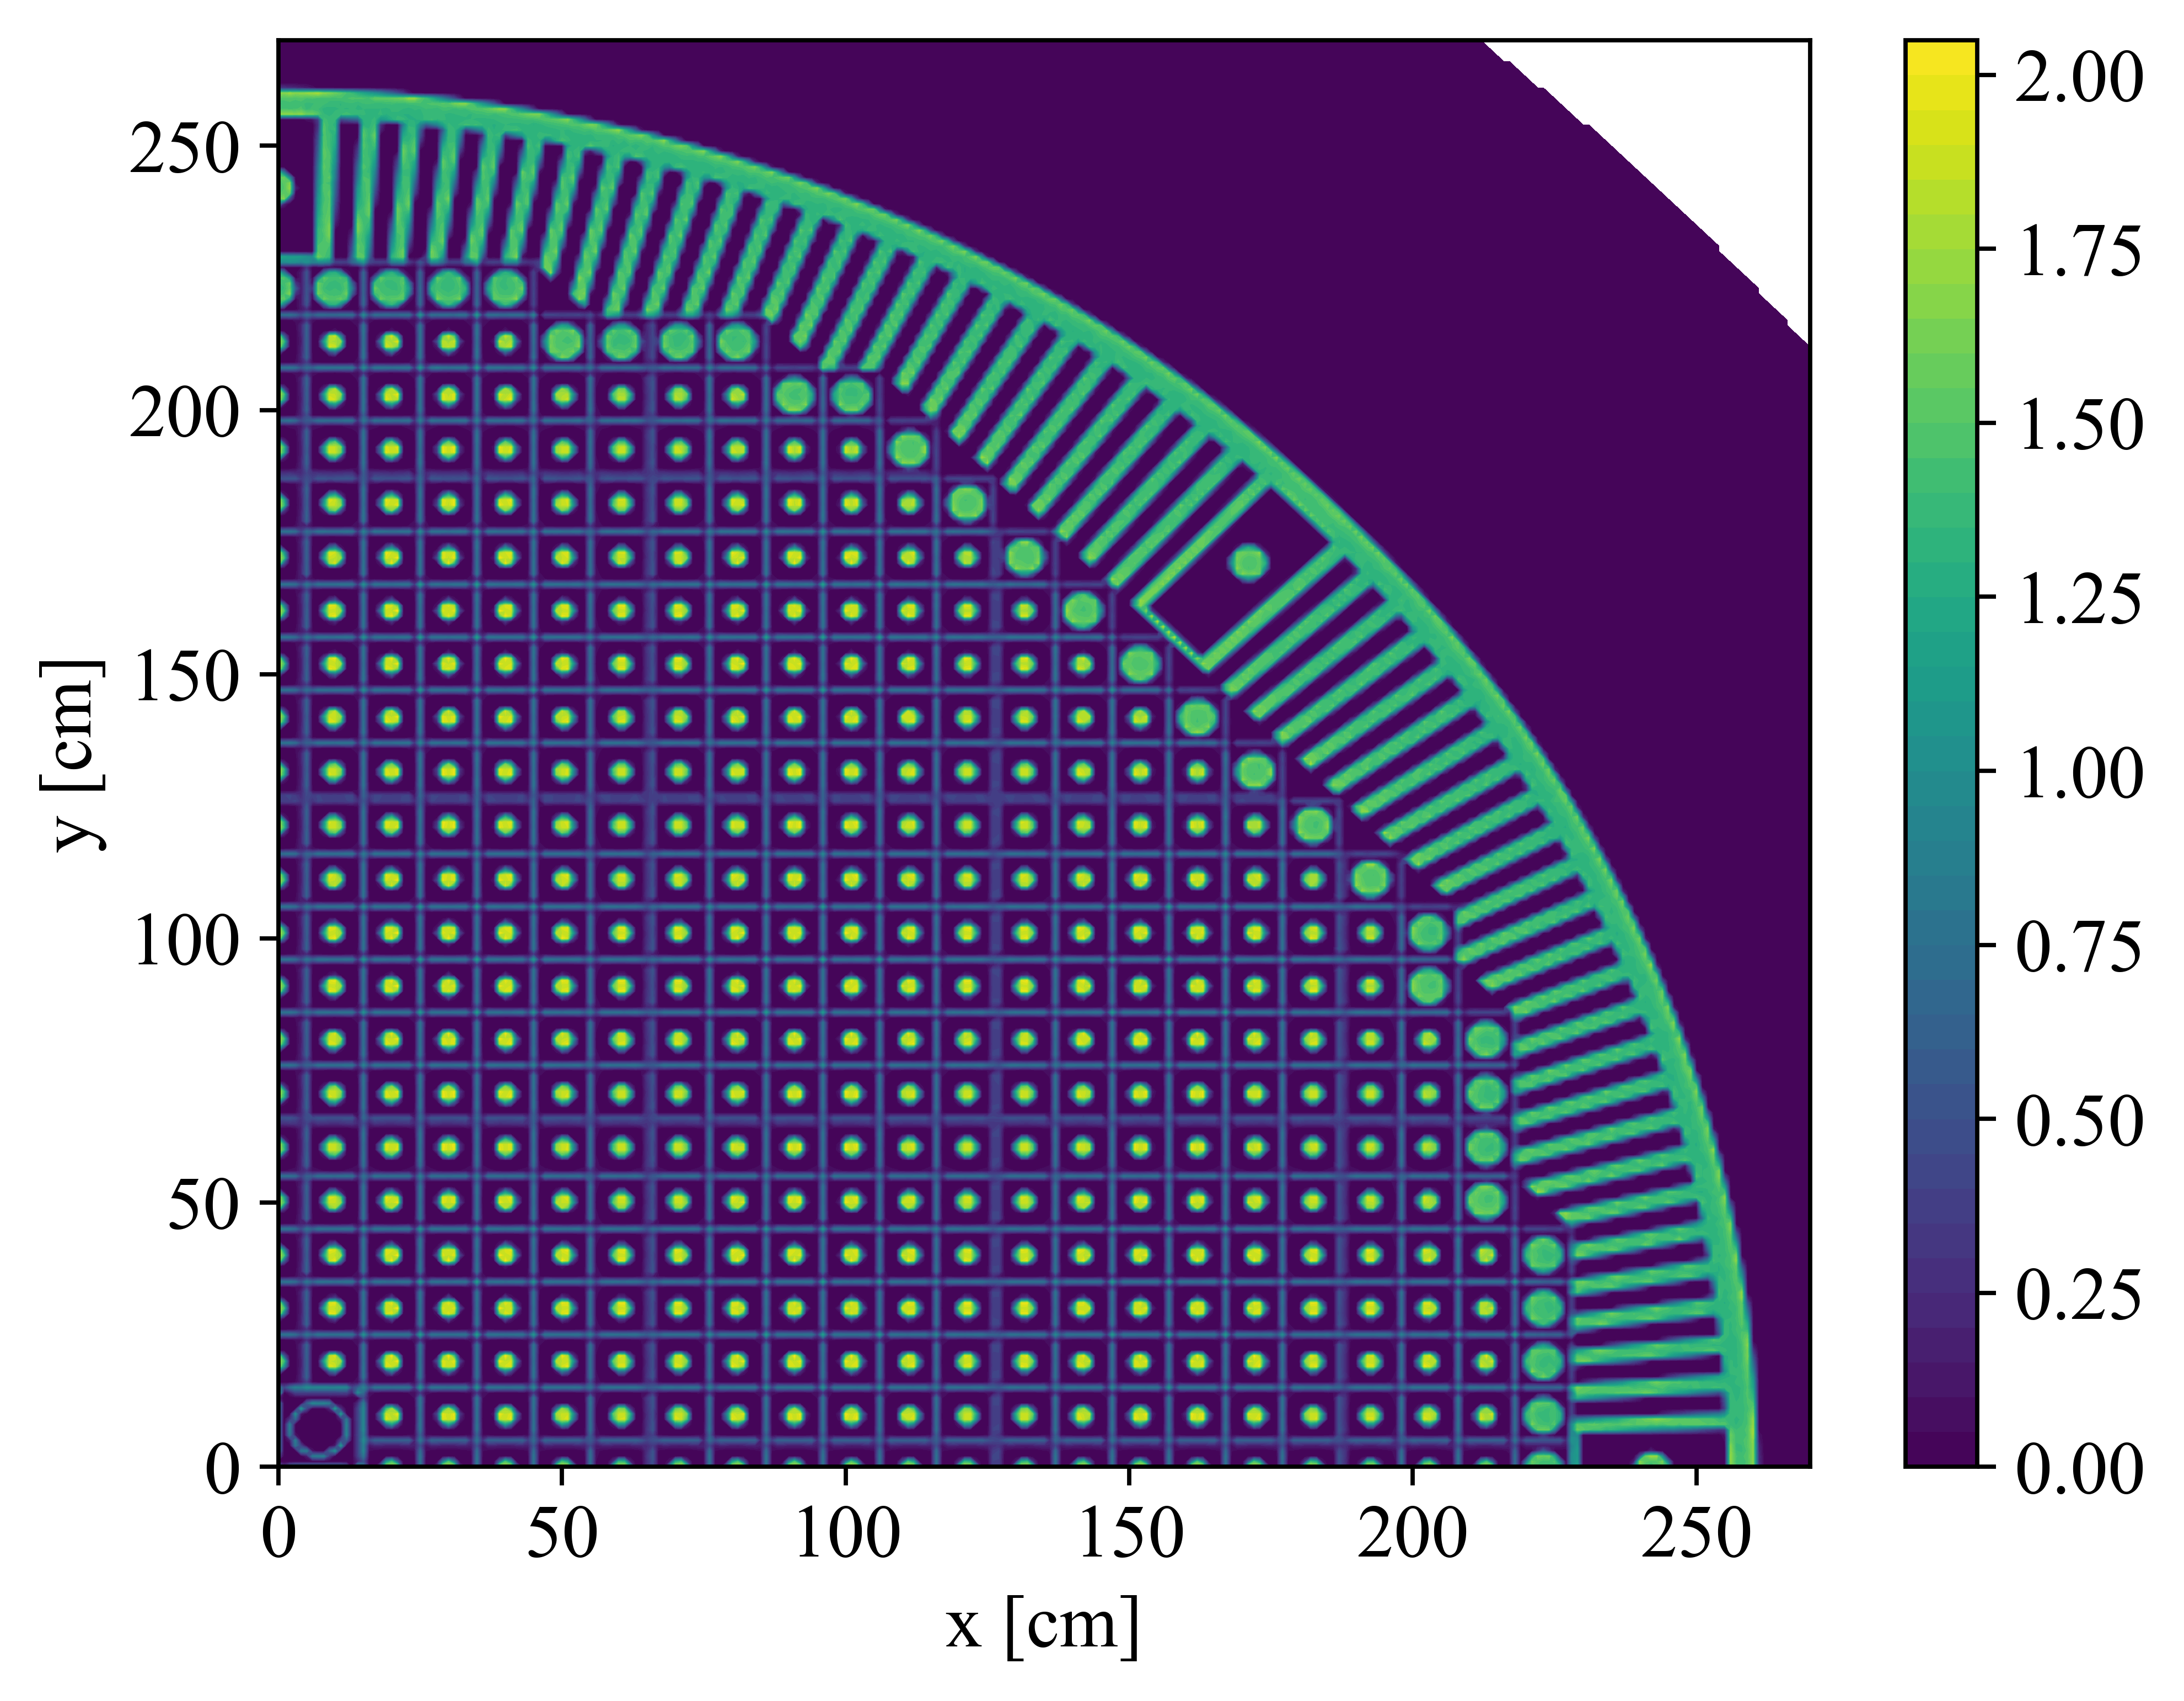
\includegraphics[width=\textwidth]{breeding_distribution_eq.png} 
  \caption{$^{232}$Th neutron capture reaction rate normalized by total flux 
  for equilibrium fuel salt composition.}
  \label{fig:breeding_den}
\end{figure}
\subsection{Temperature coefficient of reactivity}
Table~\ref{tab:tcoef} summarizes temperature effects on reactivity calculated 
in this work for both initial and equilibrium fuel compositions, compared 
with the original \gls{ORNL} report data \cite{robertson_conceptual_1971}. 
Uncertainty for each temperature coefficient also appears in 
Table~\ref{tab:tcoef}. The main physical principle underlying the reactor 
temperature feedback is an expansion of material that is heated. When the fuel 
salt temperature increases, the density of the salt decreases, but at the same 
time, the total volume of fuel salt in the core remains constant because it is 
bounded by the graphite. When the graphite temperature increases, the density 
of graphite decreases, creating additional space for fuel salt. To determine 
the temperature coefficients, the cross section temperatures for the fuel and 
moderator were changed from 900K to 1000K. Three different cases were considered:
\begin{enumerate}
  \item Temperature of fuel salt rising from 900K to 1000K.
  \item Temperature of graphite rising from 900K to 1000K.
  \item Whole reactor temperature rising from 900K to 1000K.
\end{enumerate}
%%%%%%%%%%%%%%%%%%%%%%%%%%%%%%%%%%%%%%%%
\begin{table}[ht!]
  \centering
  \caption{Temperature coefficients of reactivity for initial and equilibrium 
  state.}
\begin{tabularx}{\textwidth}{ m | s | s | x } \hline
   Reactivity coefficient [pcm/K]  & Initial      & Equilibrium  & Reference 
        \cite{robertson_conceptual_1971} \\  \hline
Fuel salt        & $-3.22\pm0.044$ & $-1.53\pm0.046$ & $-3.22$  \\
Moderator        & $+1.61\pm0.044$ & $+0.97\pm0.046$ & $+2.35$  \\
Total            & $-3.1\pm0.04$   & $-0.97\pm0.046$ & $-0.87$  \\ \hline
\end{tabularx}
  \label{tab:tcoef}
\end{table}
%%%%%%%%%%%%%%%%%%%%%%%%%%%%%%%%%%%%%%%%%%%%%%%%%%%%%%%%%%%%%%%%%%%%%%%%%%%%%%%%
In the first case, changes in the fuel temperature only impact fuel density. In 
this case, the geometry is unchanged because the fuel is a liquid. However, 
when the moderator heats up, both the density and the geometry change due to 
thermal expansion of the solid graphite blocks and reflector. Accordingly, the 
new graphite density was calculated using a linear temperature expansion 
coefficient of 1.3$\times10^{-6}$K$^{-1}$ \cite{robertson_conceptual_1971}. A new 
geometry input was created based on this information.

The fuel temperature coefficient (FTC) is negative for both initial and 
equilibrium fuel compositions due to thermal Doppler broadening of the resonance 
capture cross sections in the thorium. This is in good agreement with earlier 
research \cite{robertson_conceptual_1971,park_whole_2015}. The moderator 
temperature coefficient (MTC) is positive for the startup composition and decreases 
during reactor operation because of spectrum hardening with fuel depletion. 
Finally, the total temperature coefficient of reactivity is negative for both 
cases, but decreases during reactor operation due to spectral shift. In 
summary, even after 20 years of operation the total temperature coefficient of 
reactivity is relatively large and negative during reactor operation, despite 
positive MTC, and affords excellent reactor stability and control.

\subsection{Reactivity control system rod worth}
Table~\ref{tab:rod_worth} summarizes the reactivity control system worth. 
During normal operation, the control (graphite) rods are fully inserted, and the 
safety (B$_4$C) rods are fully withdrawn. To insert negative reactivity into 
the core, the graphite rods are gradually withdrawn from the core. In an 
accident, the safety rods would be dropped down into the core. The integral rod 
worths were calculated for various positions to separately estimate the worth
of the control graphite rods\footnote{In \cite{robertson_conceptual_1971}, the 
graphite rods are referred to as ``control'' rods.}, the safety (B$_4$C) rods, 
and the whole reactivity control system. Control rod integral worth is 
approximately 28 cents and stays almost constant during reactor operation. The 
safety rod integral worth decreases by  16.2\% during 20 years of operation 
because of neutron spectrum hardening and absorber accumulation in proximity to 
reactivity control system rods. This 16\% decline in control system worth 
should be taken into account in \gls{MSBR} accident analysis and safety 
justification.
%%%%%%%%%%%%%%%%%%%%%%%%%%%%%%%%%%%%%%%%
\begin{table}[ht!]
  \centering
  \caption{Control system rod worth for initial and equilibrium fuel 
  composition.}
\begin{tabularx}{\textwidth}{ b | x | x } \hline
Reactivity parameter [cents]  &  Initial      &  Equilibrium      \\ \hline
Control (graphite) rod integral worth               & $\ 28.2\pm0.8$    & $\ 
        29.0\pm0.8$ \\ Safety (B$_4$C) rod integral worth                  & 
        $251.8\pm0.8$    & $211.0\pm0.8$  \\
Total reactivity control system worth               & $505.8\pm0.7$    & 
        $424.9\pm0.8$ \\ \hline
\end{tabularx}
  \label{tab:rod_worth}
\end{table}
%%%%%%%%%%%%%%%%%%%%%%%%%%%%%%%%%%%%%%%%%%%%%%%%%%%%%%%%%%%%%%%%%%%%%%%%%%%%%%%%

\subsection{Six Factor Analysis}
The effective multiplication factor can be expressed using the following formula:
\begin{align*}
k_{eff} = k_{inf} P_f  P_t = \eta \epsilon p f P_f P_t
\end{align*}

Table~\ref{tab:six_factor} summarizes the six factors for both initial and 
equilibrium fuel salt composition. The non-leakage probability for both fast 
and thermal neutrons does not change during reactor operation because these 
values are not largely affected by the neutron spectrum shift. In contrast, 
neutron reproduction factor ($\eta$), resonance escape probability (p), and 
fast fission factor ($\epsilon$) are considerably different between startup and 
equilibrium. As indicated in Figure~\ref{fig:spectrum}, the neutron spectrum is 
softer at the beginning of reactor life. Neutron spectrum hardening causes the fast 
fission factor to increase through the core lifetime. The opposite is true for the 
resonance escape probability. Finally, the neutron reproduction factor 
decreases during reactor operation due to accumulation of fissile plutonium 
isotopes.
%%%%%%%%%%%%%%%%%%%%%%%%%%%%%%%%%%%%%%%%
\begin{table}[hb!]
  \centering
  \caption{Six factors for the full-core \gls{MSBR} model for initial and 
  equilibrium fuel composition.}
\begin{tabularx}{\textwidth}{ b | s | s } \hline
Factor  & Initial      & Equilibrium   \\ \hline
Neutron reproduction factor ($\eta$)     & $1.3960\pm.000052$     & 
        $1.3778\pm.00005$ \\ Thermal utilization factor (f)           & 
        $0.9670\pm.000011$     & $0.9706\pm.00001$ \\
Resonance escape probability (p)         & $0.6044\pm.000039$     & 
        $0.5761\pm.00004$ \\
Fast fission factor ($\epsilon$)         & $1.3421\pm.000040$     & 
        $1.3609\pm.00004$ \\
Fast non-leakage probability (P$_f$)     & $0.9999\pm.000004$     & 
        $0.9999\pm.000004$ \\
Thermal non-leakage probability (P$_t$)  & $0.9894\pm.000005$     & 
        $0.9912\pm.00005$ \\ \hline
\end{tabularx}
  \label{tab:six_factor}
\end{table}
%%%%%%%%%%%%%%%%%%%%%%%%%%%%%%%%%%%%%%%%%%%%%%%%%%%%%%%%%%%%%%%%%%%%%%%%%%%%%%%%
\subsection{Thorium refill rate}
In a \gls{MSBR} reprocessing scheme, the only external feed material flow  is 
$^{232}$Th. Figure~\ref{fig:th_refill} shows the $^{232}$Th feed rate 
calculated for 60 years of reactor operation. The $^{232}$Th feed rate 
fluctuates significantly as a result of the batch-wise nature of this online 
reprocessing approach. For example, the large spikes of up to 36 kg/day in a 
thorium consumption occurs every 3435 days. This is required due to batch-wise 
removal of strong absorbers (Rb, Sr, Cs, Ba). The corresponding effective 
multiplication factor increase (Figure~\ref{fig:keff}) and breeding 
intensification leads to additional $^{232}$Th consumption.  
\begin{figure}[ht!] % replace 't' with 'b' to force it to \centering
  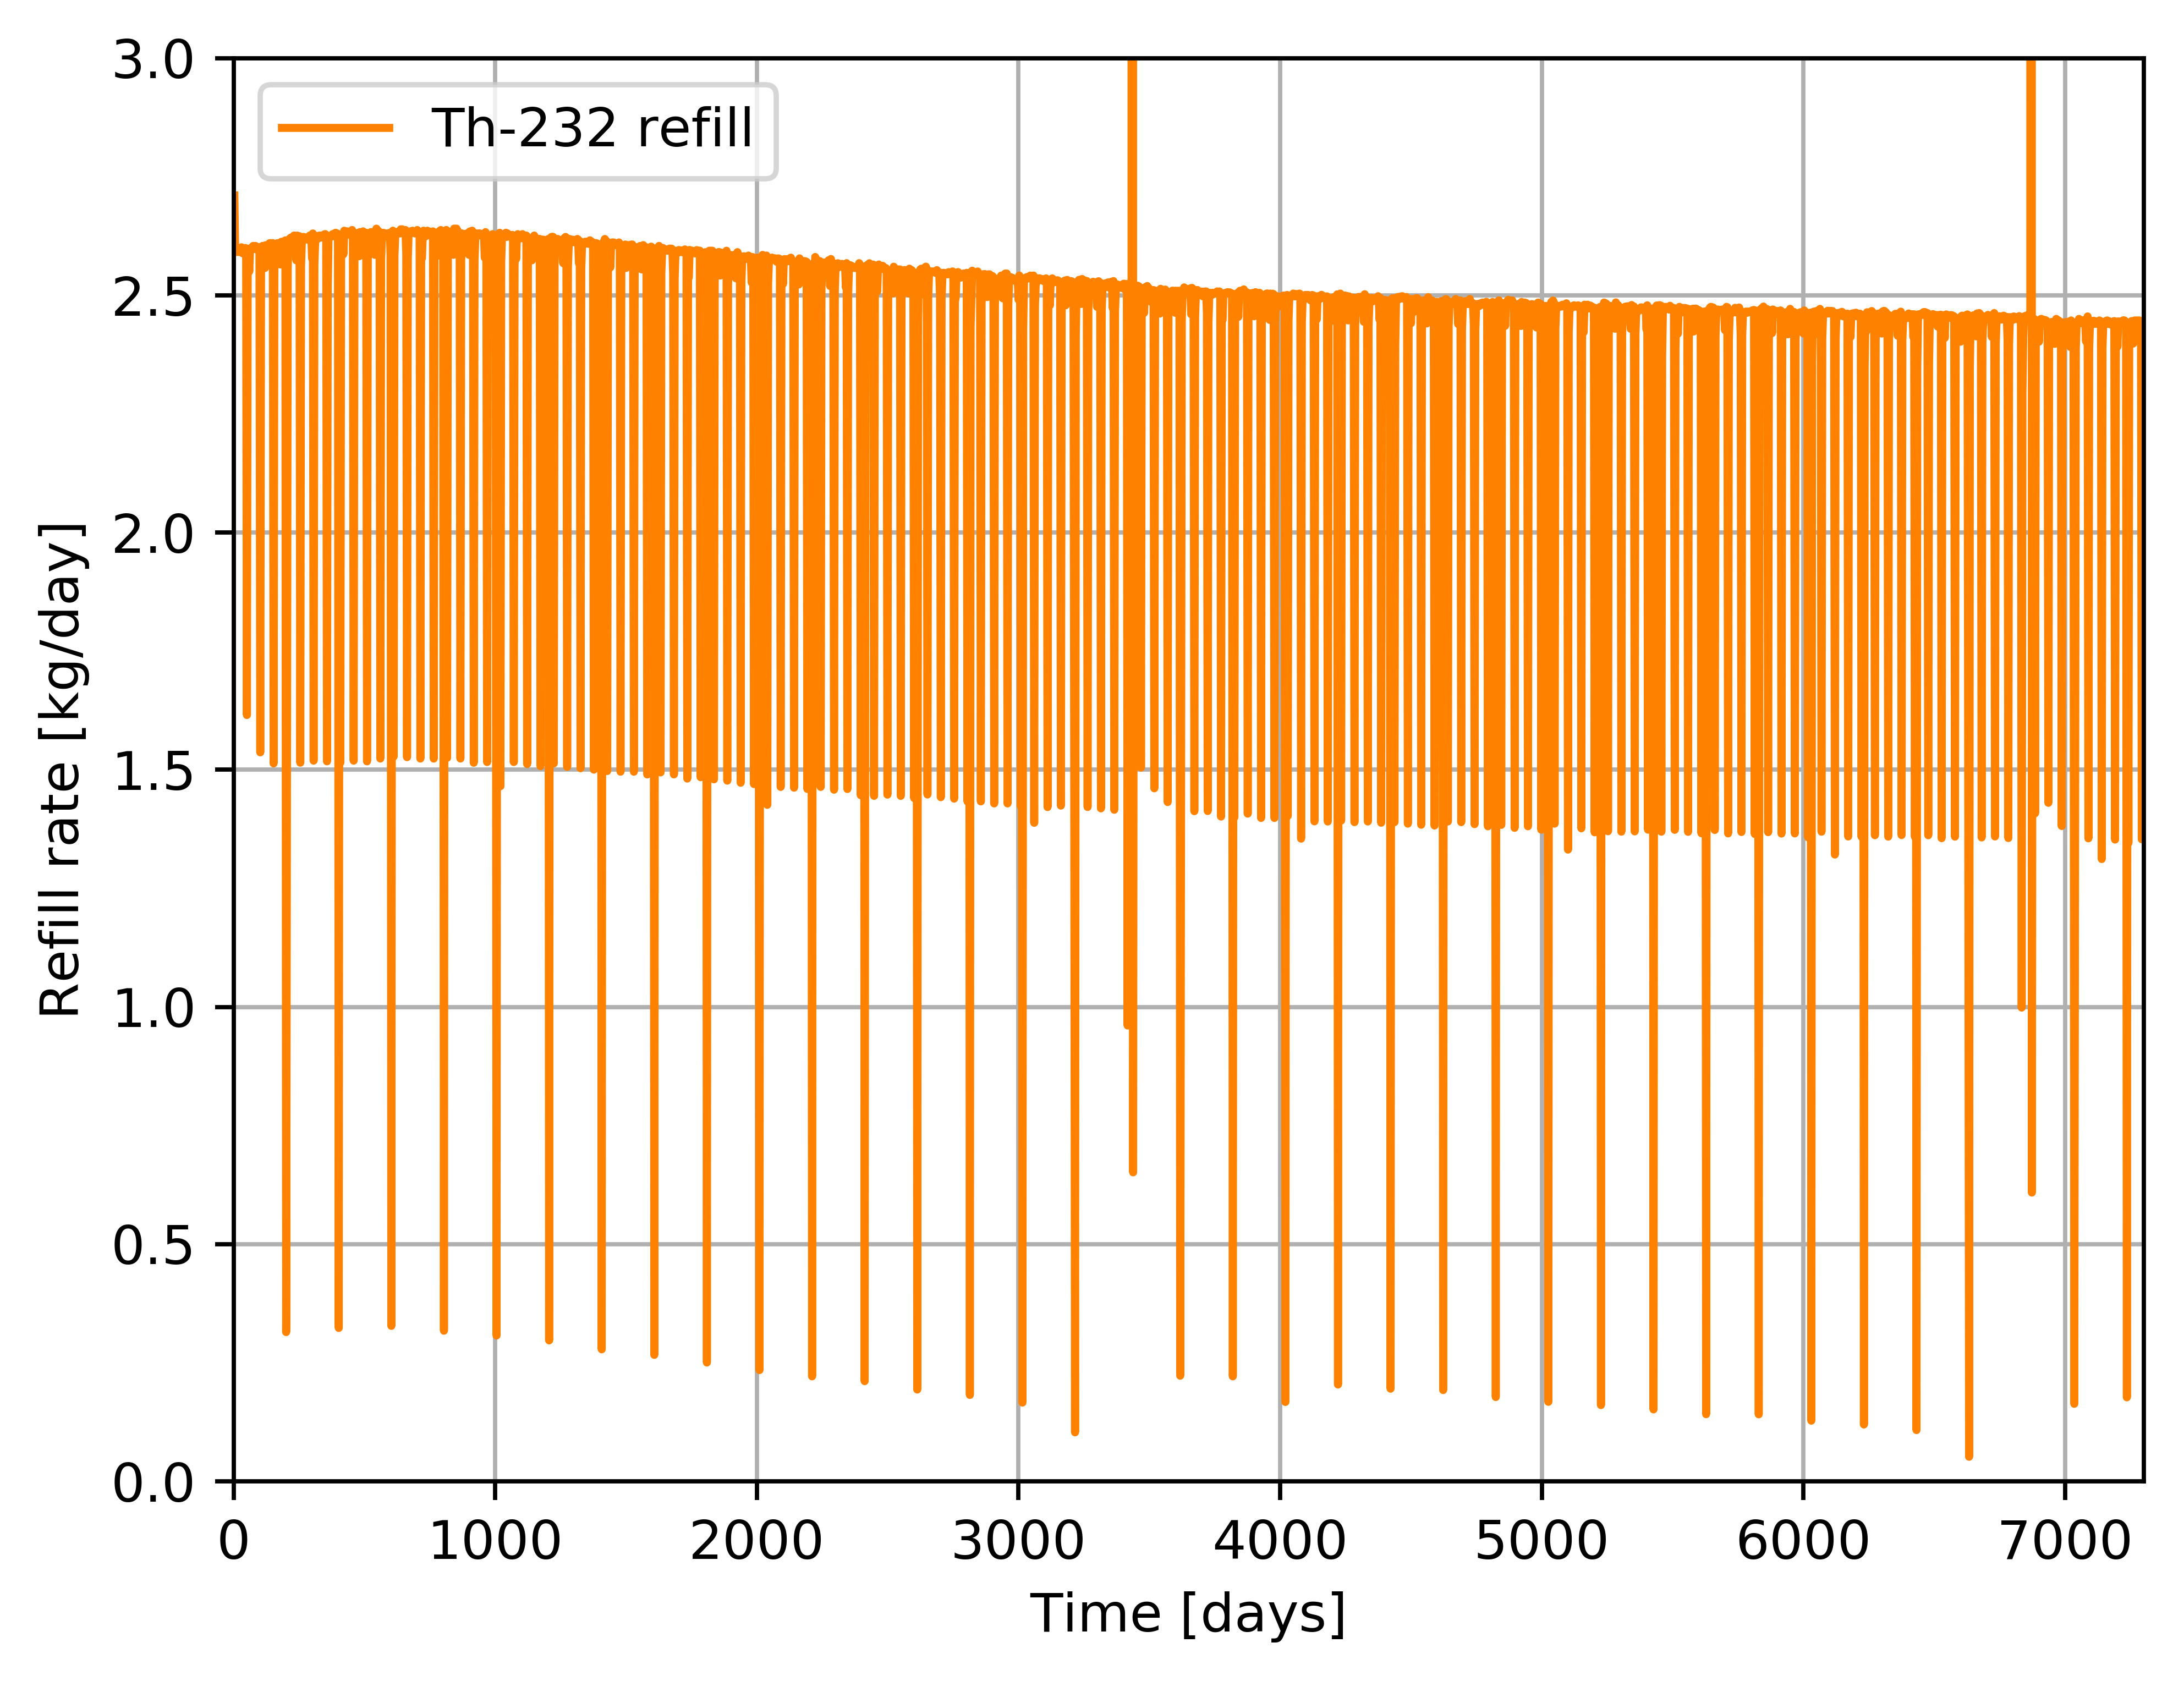
\includegraphics[width=\textwidth]{Th_refill_rate.png} \caption{$^{232}$Th 
  feed rate over 60 years of \gls{MSBR} operation.}
  \label{fig:th_refill}
\end{figure}

The average thorium feed rate increases during the first 500 days of operation, 
and steadily decreases due to spectrum hardening and accumulation of 
absorbers in the core. As a result, the average $^{232}$Th feed rate over 60 
years of operation is about 2.40 kg/day. This thorium consumption rate is in 
good agreement with a recent online reprocessing study by \gls{ORNL} 
\cite{betzler_molten_2017}.

\subsection{The effect of removing fission product from fuel salt}
Loading initial fuel salt composition into the \gls{MSBR} core leads to a 
supercritical configuration (Figure ~\ref{fig:fp_removal}). After reactor 
startup, the effective multiplication factor for the case with volatile gases 
and noble metals removal is approximately 7500 pcm  higher than for case with 
no fission products removal. This significant impact on the reactor core is
achieved due to immediate removal (20 sec cycle time) and high absorption cross 
section of Xe, Kr, Mo, and other noble metals removed. The effect of rare earth 
element removal is considerable a few months after startup and reached 
approximately 5500 pcm after 10 years of operation. The rare earth elements were 
removed at a slower rate (50-day cycle time). Moreover, 
Figure~\ref{fig:fp_removal} demonstrates that batch-wise removal of strong 
absorbers every 3 days did not necessarily leads to fluctuation in results 
but rare earth elements removal every 50 days causes an approximately 600 pcm jump 
in reactivity.

The effective multiplication factor of the core reduces gradually over 
operation time because the fissile material ($^{233}$U) continuously depletes 
from the fuel salt due to fission while fission products 
accumulate in the fuel salt simultaneously. Eventually, without fission products removal, 
the reactivity decreases to the subcritical state after approximately 500 and 
1300 days of operation for cases with no removal and volatile gases \& noble 
metals removal, respectively. The time when the simulated core reaches 
subcriticality ($k_{eff}<$1.0) for full-core model) is called the core lifetime. 
Therefore, removing fission products provides with significant neutronic benefit 
and enables a longer core lifetime.
\begin{figure}[ht!] % replace 't' with 'b' to force it to 
  \centering
  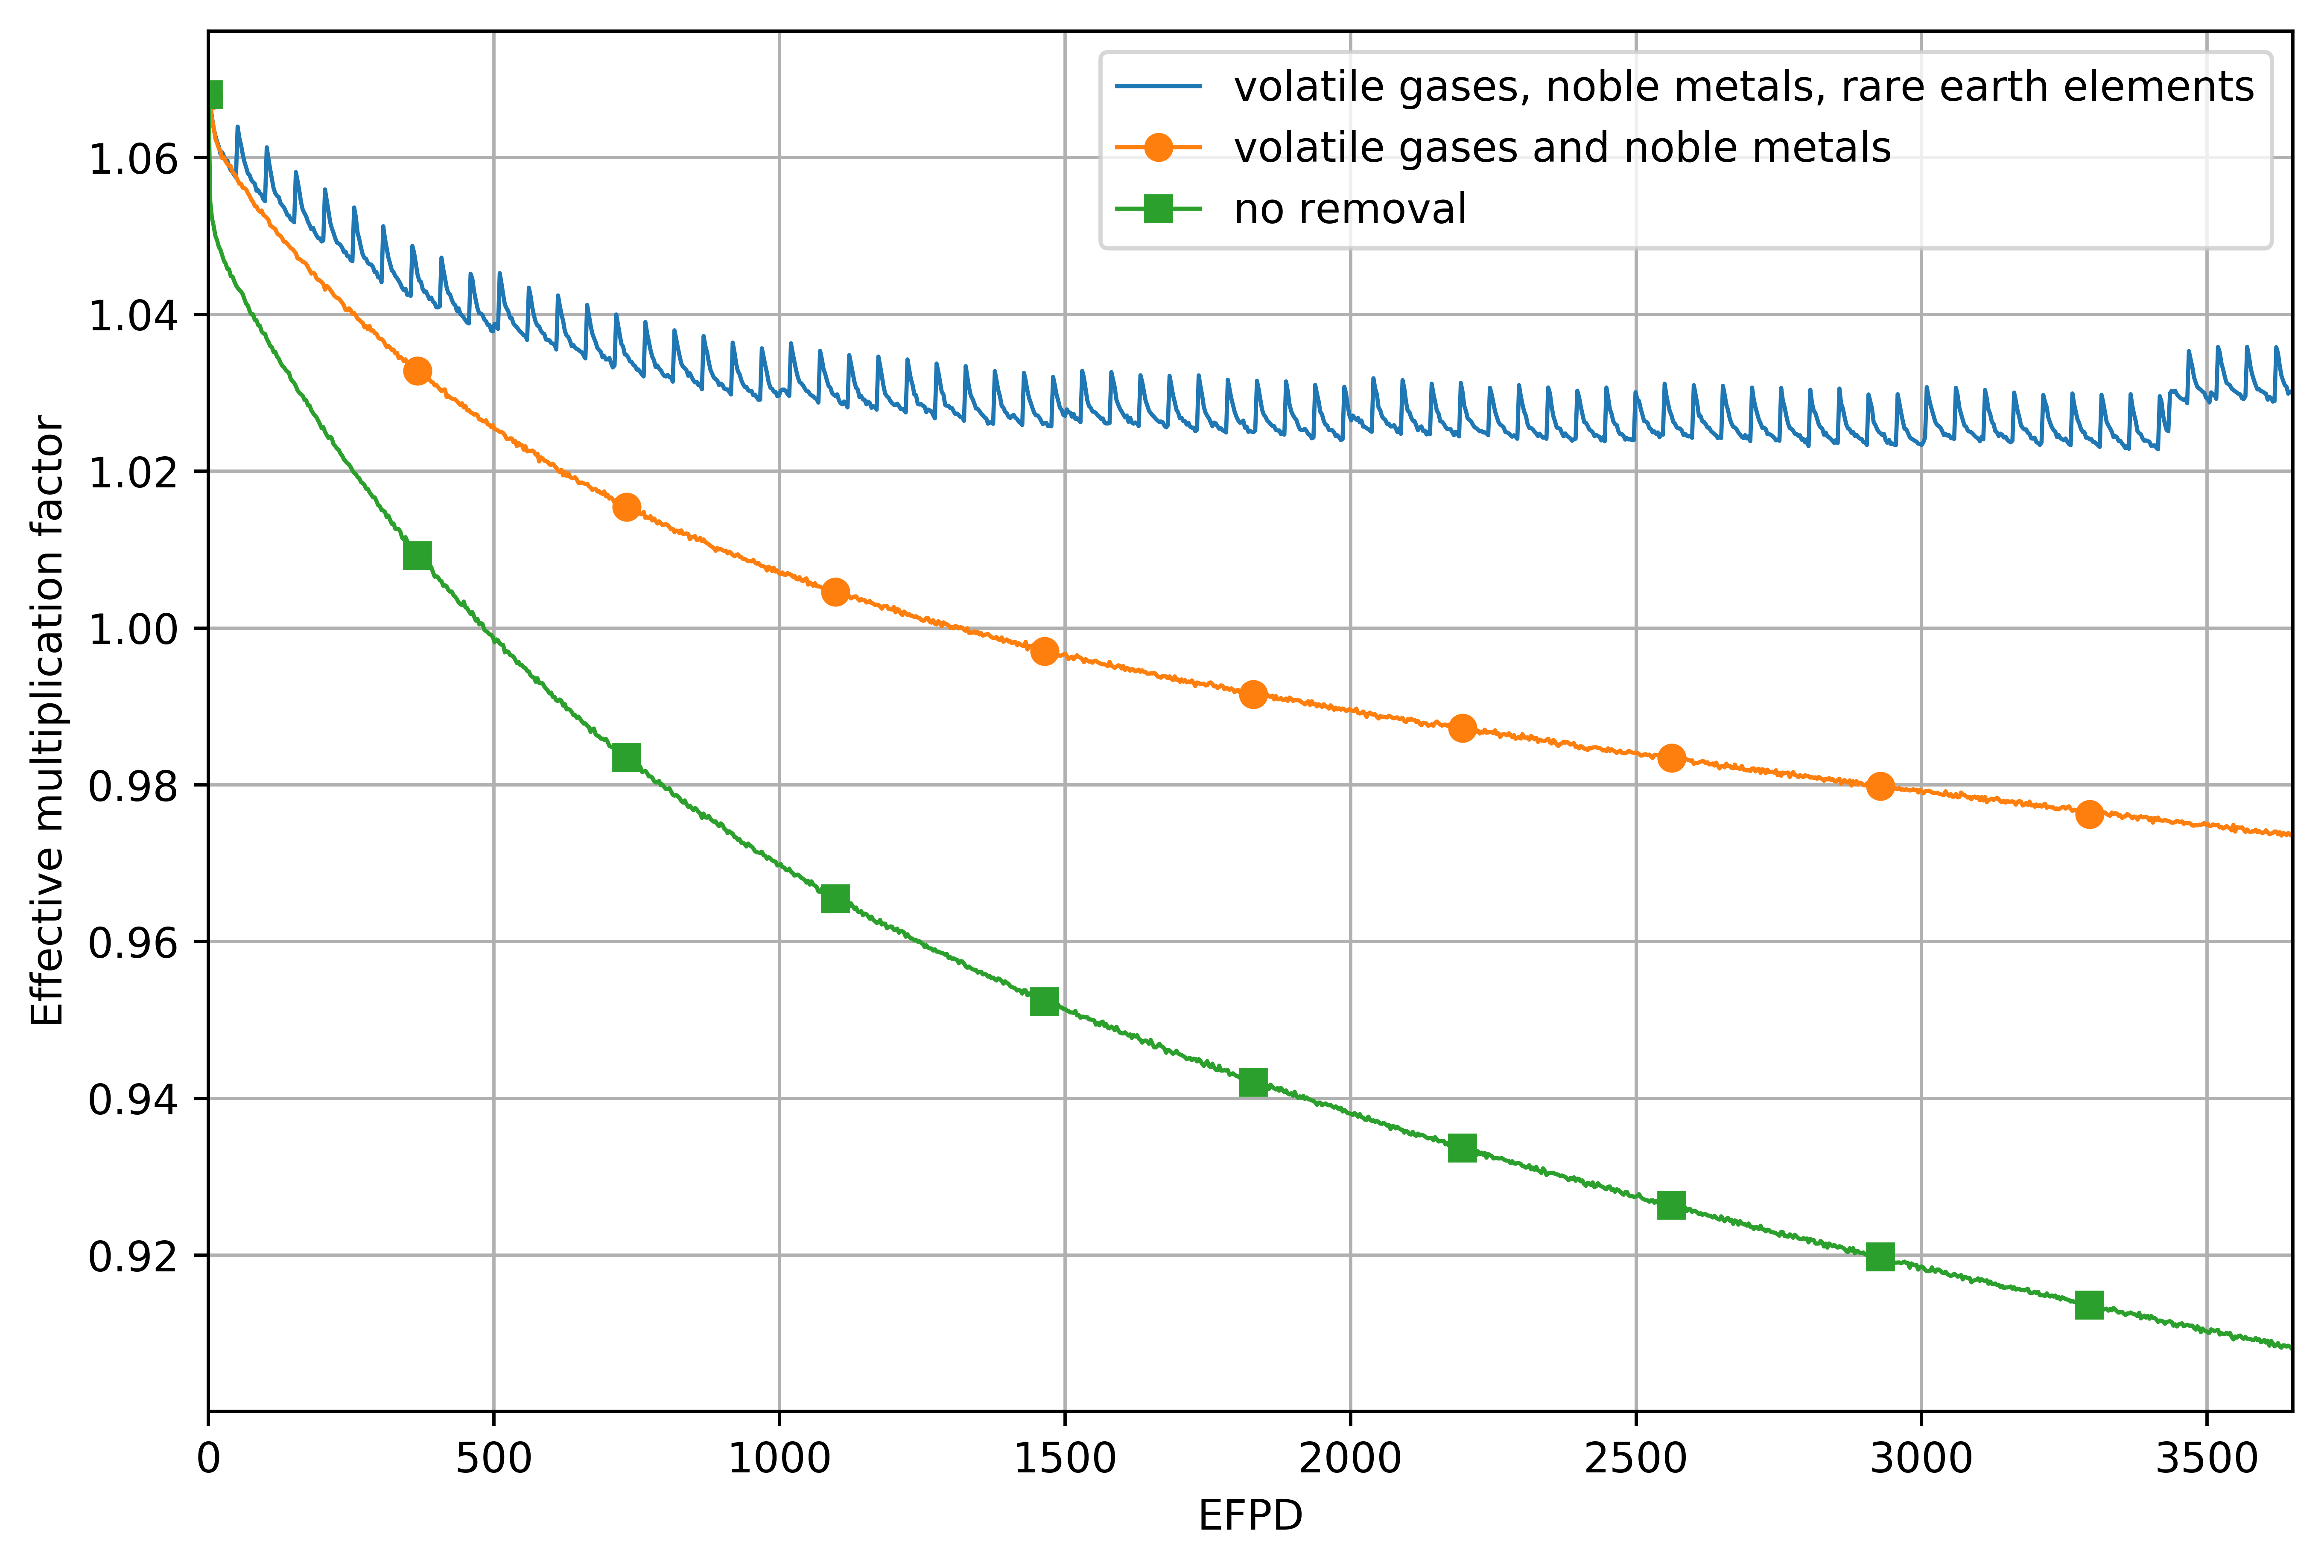
\includegraphics[width=\textwidth]{keff_rem_cases.png} 
  \caption{Calculated effective multiplication factor for full-core \gls{MSBR} 
model with removal of various fission product groups over 10 years of 
operation.}
  \label{fig:fp_removal}
\end{figure}

\FloatBarrier
%\section{Discussion}
% This should explore the significance of the results of the work, not repeat
% them. A combined Results and Discussion section is often appropriate. Avoid
% extensive citations and discussion of published literature.



%\FloatBarrier
\section{Discussion and conclusions}

This work introduces the open source \gls{MSR} simulation package SaltProc. 
SaltProc expands the capability of SERPENT 2, the continuous-energy Monte Carlo 
code to include online reprocessing in liquid-fueled \gls{MSR} operation 
\cite{andrei_rykhlevskii_arfc/saltproc:_2018}. Benefits of SaltProc include 
generic geometry modeling, multi-flow capabilities, time-dependent feed and 
removal rates, and the ability to specify removal efficiency. The main goal of 
this work has 
been to demonstrate SaltProc's capability to find the equilibrium fuel salt 
composition (where equilibrium is defined as when the number densities of major 
isotopes vary less than 1\% over several years). A secondary goal has been to 
compare predicted operational and safety parameters (e.g., neutron energy 
spectrum, power and breeding distribution, temperature coefficients of 
reactivity) of the \gls{MSBR} at startup and equilibrium state. A tertiary goal 
has been to demonstrate benefits of continuous fission products removal for 
thermal \gls{MSR} design.

Toward these goals, a full-core high-fidelity benchmark model of the \gls{MSBR} 
was implemented in SERPENT 2. The purpose of the full-core model instead of 
the simplified single-cell model \cite{betzler_molten_2017, 
rykhlevskii_online_2017, betzler_fuel_2018} was to precisely describe the 
two-region \gls{MSBR} concept design sufficiently to accurately represent 
breeding in the outer core zone. When running depletion calculations, the most 
important fission products and $^{233}$Pa are removed while fertile and fissile 
materials are added to the fuel salt every 3 days.  Meanwhile, the removal 
interval for the rare earths, volatile fluorides, and seminoble metals was more 
than month which caused effective multiplication factor fluctuation. 

\subsection{Equilibrium state search}
The results of this study indicate that the effective multiplication factor 
slowly decreases from 1.075 and reaches 1.02 at equilibrium after approximately 
6 years of operation. At the same time, the concentration of $^{233}$U, $^{232}$Th, 
$^{233}$Pa, $^{232}$Pa stabilizes after approximately 2500 days of operation. 
Particularly, $^{233}$U number density equilibrates\footnote{fluctuates less 
than 0.8\%} after 16 years of operation. Consequently, the core reaches the quasi-equilibrium state 
after 16 years of operation. However, a wide variety of nuclides, 
including fissile isotopes (e.g. $^{233}$U, $^{239}$Pu) and non-fissile strong 
absorbers (e.g. $^{234}$U), continue accumulating in the core. The current work results 
show that a true equilibrium composition cannot exist but the balance
between strong absorber accumulation and new fissile material 
production can be achieved to keep the reactor critical.

\subsection{Spectral shift}
We also found that the neutron energy spectrum grows harder as equilibrium 
approaches because significant heavy fission products accumulate in 
the \gls{MSBR} core. Moreover, the neutron energy spectrum in the central core 
region is much softer than in the outer core region due to lower 
moderator-to-fuel ratio in the outer zone, and this distribution remains stable 
during reactor operation. Finally, the epithermal or thermal spectrum is needed 
to effectively breed $^{233}$U from $^{232}$Th because radiative capture cross 
section of thorium-232 monotonically decreases from $10^{-10}$ MeV to $10^{-5}$ 
MeV. A harder spectrum in the outer core region tends to significantly increase 
resonance absorption in thorium and decrease the absorptions in fissile and 
structural materials. 

The spatial power distribution in the \gls{MSBR} shows that 98\% of the fission 
power is generated in central zone I, and neutron energy spectral shift did not 
cause any notable changes in a power distribution. The spatial distribution of 
neutron capture reaction rate for fertile $^{232}$Th, corresponding to breeding in 
the core, confirms that most of the breeding occurs in an outer, 
undermoderated, region of the \gls{MSBR} core. Finally, the average $^{232}$Th 
refill rate throughout 60 years of operation is approximately 2.40 kg/day or 
100 g/GWh$_e$.

We compared the safety parameters for the initial fuel loading and 
equilibrium compositions using the SERPENT 2 Monte Carlo code. 
The total temperature coefficient 
is large and negative at startup and equilibrium but the magnitude decreases 
throughout reactor operation from $-3.10$ to $-0.94$ pcm/K as the spectrum 
hardens. The moderator 
temperature coefficient is positive and also decreases during fuel depletion. 
The reactivity control system efficiency analysis showed that the safety rod integral 
worth decreases by approximately 16.2\% over 16 years of operation, while 
graphite rod integral worth remains constant. Therefore, neutron energy 
spectrum hardening during fuel salt depletion has an undesirable impact on 
\gls{MSBR} stability and controllability, and should be taken into 
consideration in further analysis of transient accident scenarios.

\subsection{Benefits of fission product removal}

The \gls{MSBR} core performance benefits from the removal of volatile gases, 
noble metals, and rare earths from the fuel salt. 
Moreover, immediate removal of volatile gases (e.g., xenon) and noble metals 
increased reactivity by approximately 7500 pcm over a 10-year 
timeframe. In contrast, the effect of relatively slower removal of rare earth 
elements (every 50 days cycle instead of 3 days) has less impact (5500 pcm) on 
the core reactivity after 10 years of operation. An additional study 
is needed to establish neutronic  and economic tradeoffs of removing each element.

\subsection{Future work}
Continued SaltProc-SERPENT coupled simulation efforts could progress in a 
number of different directions. First optimization of reprocessing parameters (e.g. time step, feeding rate, 
protactinium removal rate) could establish the best fuel utilization, breeding 
ratio, or safety characteristics for various designs. This might be performed with a parameter sweeping 
outer loop which would change an input parameter by a small increment, run the 
simulation and analyze output to determine optimal configuration. Alternatively, 
the existing RAVEN optimization framework \cite{alfonsi_raven_2013} might be 
employed for such optimization studies.

Only the batch-wise online reprocessing approach has been treated in this 
work. However, the SERPENT 2 Monte Carlo code was recently extended for 
continuous online fuel reprocessing simulation \cite{aufiero_extended_2013}. 
This extension must be verified against existing SaltProc/SERPENT or 
ChemTriton/SCALE packages, and could be employed for immediate removal of 
fission product gases (e.g., Xe, Kr) which have a strong negative impact on 
core lifetime and breeding efficiency. Finally, using the built-in SERPENT 2 
Monte Carlo code online reprocessing \& refueling material burnup routine would 
significantly speed up computer-intensive full-core depletion simulations.

\FloatBarrier
\section{Acknowledgments}

This research is part of the Blue Waters sustained-petascale computing project, 
which is supported by the National Science Foundation (awards OCI-0725070 and 
ACI-1238993) and the state of Illinois. Blue Waters is a joint effort of the 
University of Illinois at Urbana-Champaign and its National Center for 
Supercomputing Applications 

The authors would like to thank  members of Advanced Reactors and Fuel Cycles
research group (ARFC) at the University of Illinois - Urbana Champaign who 
provided valuable code reviews and proofreading.

The authors contributed to this work as described below.  Andrei Rykhlevskii 
conceived and designed the simulations, wrote the paper, prepared figures 
and/or tables, performed the computation work, contributed to the software 
product, and reviewed drafts of the paper. Mr. Rykhlevskii is supported by the 
Department of Nuclear, Plasma, and Radiological Engineering.

Kathryn D. Huff directed and 
supervised the work, conceived and designed the simulations, wrote the paper, 
contributed to the software product, and reviewed drafts of the paper.  Prof. 
Huff is supported by the Nuclear Regulatory Commission Faculty Development 
Program, the National Center for Supercomputing Applications, the NNSA Office 
of Defense Nuclear Nonproliferation R\&D through the Consortium for Verfication 
Technologies and the Consortium for Nonproliferation Enabling Capabilities, and 
the International Institute for Carbon Neutral Energy Research (WPI-I2CNER), 
sponsored by the Japanese Ministry of Education, Culture, Sports, Science and 
Technology.

\FloatBarrier

%\nocite{robertson_conceptual_1971} % placeholder until citations appear
\bibliography{2018-msbr-reproc}

\end{document}
